\documentclass[17pt,a4paper,twoside]{extbook}




\usepackage[left=1in,right=1in]{geometry}
\usepackage{float}
\usepackage{enumitem}
\usepackage{fancyhdr}
\usepackage{pifont}
\usepackage{commath}
\usepackage{mathtools}
\usepackage[scr]{rsfso}
\usepackage[makeroom]{cancel}
\usepackage{fancybox,framed}
\usepackage{stackengine}
\usepackage{amssymb,amsmath}
\usepackage{amsthm}
%\usepackage{unicode-math}
\usepackage{esint}
\usepackage[overload]{empheq}
\usepackage{cases} 
\usepackage{accents} 
\usepackage[symbol]{footmisc}
\usepackage{cancel}
\usepackage{wrapfig}
\usepackage{graphicx}
\usepackage{subfigure}
\usepackage{xcolor}
\graphicspath{ {figures/} }
\usepackage[titletoc]{appendix}

\usepackage{pdfpages}

\newcommand{\q}[1]{``#1''}


\renewcommand{\thefootnote}{\fnsymbol{footnote}}






\theoremstyle{definition}
\newtheorem{definition}{Definition}[section]
\newtheorem*{example}{Example}
\newtheorem*{exercise}{Exercise}
\newtheorem*{solution}{Solution}
\newtheorem*{notation}{Notation}
\newtheorem*{note}{Note}
\newtheorem*{remark}{Remark}

%\newtheorem*{claimproof}{Proof of claim \theclaim}
%\newtheorem*{theoremproof}{Proof of theorem \thetheorem}






\theoremstyle{plain}
\newtheorem{theorem}{Theorem}[section]
\newtheorem{lemma}{Lemma}[section]
\newtheorem{claim}{Claim}[section]
\newtheorem{axiom}{Axiom}[section]



%\usepackage[thmmarks]{ntheorem}


%\theorembodyfont{\normalfont}
%\newtheorem{definition}{Definition}[section]
%\theoremstyle{plain}
%\theorembodyfont{\normalfont}
%\newtheorem{example}{Example}
%\theoremstyle{nonumberplain}
%\newtheorem{notation}{Notation}
%
%\theorembodyfont{\itshape}
%\theoremstyle{plain}
%\newtheorem{theorem}{Theorem}
%\newtheorem{lemma}[theorem]{Lemma}
%
%\newtheorem{claim}{Claim}[theorem]
%\theoremstyle{nonumberplain}
%\theoremsymbol{\ensuremath{\Box}}
%\newtheorem{proof}{Proof}
%\theoremsymbol{\ensuremath{\blacksquare}} 
%\newtheorem{claimproof}{Proof of claim \theclaim}

% argumented matrix
\makeatletter
\renewcommand*\env@matrix[1][*\c@MaxMatrixCols c]{%
  \hskip -\arraycolsep
  \let\@ifnextchar\new@ifnextchar
  \array{#1}}
\makeatother
%

% volume
\makeatletter
\DeclareRobustCommand{\volume}{\text{\volumedash}V}
\newcommand{\volumedash}{%
  \makebox[0pt][l]{%
    \ooalign{\hfil\hphantom{$\m@th V$}\hfil\cr\kern0.08em--\hfil\cr}%
  }%
}
%
\makeatother



\title{%
Tensor Analysis with Applications in Engineering \\
  \large ME 5121 @ NCKU ME\\
  Lecture notes}

\author{Prof. Yi-Chun Wang}
\date{February 1, 2021}







\usepackage{hyperref}
\hypersetup{hidelinks,
	colorlinks=true,
	allcolors=black,
	pdfstartview=Fit,
	breaklinks=true
}

%------------Command----------------------------------------

\newcommand{\vc}[3]{\overset{#2}{\underset{#3}{#1}}}

%--------------tensor form---------------------
\stackMath
\newcommand\tenq[2][1]{%
 \def\useanchorwidth{T}%
  \ifnum#1>1%
    \stackunder[0pt]{\tenq[\numexpr#1-1\relax]{#2}}{\scriptscriptstyle\sim}%
  \else%
    \stackunder[1pt]{#2}{\scriptscriptstyle\sim}%
  \fi%
}

%-----------------------------------------

\DeclareMathOperator\erf{erf}
\DeclareMathOperator\erfc{erfc}

\DeclareMathOperator\Arg{Arg}
\DeclareMathOperator\Log{Log}

\DeclareMathOperator\arcsec{arcsec}
\DeclareMathOperator\arccot{arccot}
\DeclareMathOperator\arccsc{arccsc}
\DeclareMathOperator\tr{tr}

\def\Res{\mathop{\text{Res}}\limits}

\setlength{\headheight}{85.0pt}

\begin{document}

\frontmatter

\maketitle


\pagenumbering{Roman}
%\pagestyle{empty}
%\pagenumbering{gobble}
\pagestyle{fancy}
\fancyhf{}
\fancyhead[C]{\textbf{\leftmark}}
\fancyfoot[C,CO]{\thepage}
\tableofcontents

%\listoffigures

%\newpage
%\pagestyle{empty}

\newpage
\mainmatter
\pagenumbering{arabic}
\pagestyle{fancy}
%\setcounter{page}{1}
\fancyhf{}
\fancyhead[CO]{\textbf{\leftmark}}
\fancyhead[CE]{\textbf{\rightmark}}
%\fancyhead[C]{\textbf{\leftmark}}
%\fancyhead[C]{\textbf{\rightmark}}
\fancyfoot[C,CO]{\thepage}
\fancyfoot[L,L]{\footnotesize Prof. Yi-Chun Wang}
\renewcommand{\footrulewidth}{1pt}

\raggedright




\chapter{Reviews on Euclidean space}
\begin{definition}


A Euclidean space is defined as an $N$-dimensional vector space, denoted by $E_N$, in which
\begin{enumerate}[label=(\alph*)]
\item The inner product operation between two vectors is defined. 
\item The metric (or norm), that is, the square of the line element of the space, obtained by applying inner product on vectors themselves, is a positive definite quadratic form (i.e. always real and positive, vanishing only when the line elements vanishes). 
\item \label{ch1-(c)} It is possible to express the metric of $n$ squares with constant coefficients by performing a suitable coordinate transformation.
\end{enumerate}


\begin{note}
If \ref{ch1-(c)} is not permitted, the vector space is called \emph{$N$-dimensional Riemannian space}. 
\end{note}


\end{definition}


\chapter{Elements of Cartesian Tensor Analysis}

\section{Indicial notation}

Consider $\tenq{u}$ and $\tenq{v}$ which are elements of $E_3$

\[\tenq{u}\cdot\tenq{v}=u_1v_1+u_2v_2+u_3v_3=\sum_{i=1}^3u_iv_i\vc{=}{\footnotemark}{}u_iv_i\]

\footnotetext{Einstein's summation convection}

\section{Range convection}


\begin{itemize}
\item All lower cases, Latin indices (both subscripts and superscripts) have the range 1, 2, 3 or $i, j \in {1, 2, 3}$
\item All lower cases, Greek indices (both subscripts and superscripts) have the range 1, 2 or $\alpha, \beta \in {1, 2}$
\end{itemize}

\begin{enumerate}[label= e.g. \arabic*)]
\item $v_{i}-3$ elements
\item $v_{ij}-3^2$ elements
\item $v_{ijk}-3^3$ elements
\item $v_{\underbrace{ij \cdots k}_{N}}-3^N$ elements
\end{enumerate}

\section{Summation convection}

If in a monomial the same index appears \emph{twice} then summation over this index is implied unless otherwise stated.

\begin{enumerate}[label= e.g. \arabic*)]

\item
\[v_{ii}=v_{11}+v_{22}+v_{33}\]
$v_{ii}\text{ (no sum)}$ either $v_{11}$ or $v_{22}$ or $v_{33}$

\item
\[u_iv_i=u_1v_1+u_2v_2+u_3v_3=u_kv_k=u_jv_j\]

thus repeated indices are \emph{dummy}.

\item
\[a_{ij}x_j=a_{i1}x_1+a_{i2}x_2+a_{i3}x_3\]

indicial equation

\[
a_{ij}x_j=b_i\Longleftrightarrow
\left\{\begin{aligned}
& a_{11}x_1+a_{12}x_2+a_{13}x_3=b_1\\
& a_{21}x_1+a_{22}x_2+a_{23}x_3=b_2\\
& a_{31}x_1+a_{32}x_2+a_{33}x_3=b_3
\end{aligned}\right.
\]

i.e. 3 equations for $i = 1,2,3$

\[a_{ij}x_j=c_{kki}=c_{11i}+c_{22i}+c_{33i}\]

\item NONSENSE

\[a_{i}c_{ji}=b_k\]
(free or non-repeated index on either side is not same)

\[a_{ikk}x_k=c_i\]
(can not have more than two repeated indices)



\end{enumerate}

\paragraph{Rules}\mbox{}\\


\begin{enumerate}[label= (\alph*)]

\item \label{ch2-2-rules-(a)}
The same index cannot appear more than twice \emph{in the same monomial}.

\item \label{ch2-2-rules-(b)}
Free (unrepeated) indices of either side of an indicial equation must agree.
\item
Both free and repeated indicies are \emph{dummy} and may be replaced by other lower case Latin letters subject to restriction \ref{ch2-2-rules-(a)} and \ref{ch2-2-rules-(b)}.

\end{enumerate}

\section{Kronecker delta}

Set of a real numbers, denoted by $\delta_{ij}$ defined as


\[
\delta_{ij}= 
\left\{\begin{aligned} 
& 0 & & \text{if $i \neq j$}\\
& 1 & & \text{if $i=j$}\end{aligned}\right.
\]

\begin{enumerate}[label= e.g. \arabic*)]
\item $\delta_{ii}=3$
\item $\delta_{ii}$ (no sum) $=1$
\item $\delta_{ij}=\delta_{ji}$
\item $\delta_{ij}v_{j}=v_{i}$, $\delta_{ik}v_{kj}=v_{ij}$
\item $\delta_{ij}\delta_{ij}=\delta_{ii}=\delta_{jj}=3$
\item $\delta_{ij}v_{ij}=v_{ii}=v_{jj}=v_{kk}$
\item $\delta_{ik}\delta_{jr}v_{kr}=v_{ij}$
\end{enumerate}

\section{Alternating symbol}

The 27 real numbers $\epsilon_{ijk}$ defined as 

\[\epsilon_{ijk}=1\]

if ($ijk$) are an \emph{even} permutation of the ordered triplet (1 2 3).

\[\epsilon_{ijk}=-1\]

if ($ijk$) are an \emph{odd} permutation of the ordered triplet (1 2 3).


\[\epsilon_{ijk}=0\]

otherwise, i.e. at least two are the same. 

\begin{enumerate}[label= e.g. \arabic*)]
\item $\epsilon_{123}=\epsilon_{231}=\epsilon_{312}=1$
\item $\epsilon_{213}=-1$
\item $\epsilon_{121}=0$
\item $\epsilon_{333}=0$

\item $\epsilon_{ijk}=\epsilon_{jki}=\epsilon_{kij}=-\epsilon_{jik}=-\epsilon_{ikj}=-\epsilon_{kji}$
\item $\epsilon_{ijk}\epsilon_{ijk}=\underbrace{\epsilon_{1jk}\epsilon_{1jk}}_{
\begin{subarray}{l}
  \epsilon_{123}\epsilon_{123} \\
  +\epsilon_{132}\epsilon_{132}=2
  \end{subarray}
}+\epsilon_{2jk}\epsilon_{2jk}+\epsilon_{3jk}\epsilon_{3jk}=6$


\end{enumerate}

\section{Representation of \texorpdfstring{$3\times 3$}{Lg} determinants}

\[
\epsilon_{1jk}v_jw_k 
= \epsilon_{123}v_2w_3+\epsilon_{132}v_3w_2 = v_2w_3-v_3w_2 = 
\begin{vmatrix}
v_2 & v_3 \\ 
w_2 & w_3
\end{vmatrix}
\]

and 

\[
\epsilon_{2jk}v_jw_k 
= \epsilon_{213}v_1w_3+\epsilon_{231}v_3w_1 = -v_1w_3+v_3w_1 = -
\begin{vmatrix}
v_1 & v_3 \\ 
w_1 & w_3
\end{vmatrix}
\]

then 

\begin{equation}
\epsilon_{ijk}u_iv_jw_k=
\begin{vmatrix}
u_1 & u_2 & u_3 \\ 
v_1 & v_2 & v_3 \\ 
w_1 & w_2 & w_3
\end{vmatrix}\tag{$\ast$}\label{eq: 2-6-*}
\end{equation}

\begin{notation}

\[\text{matrix }\mathbf{V}\vc{=}{\footnotemark}{}[V_{ij}]=
\begin{bmatrix}
V_{11} & V_{12} & V_{13} \\ 
V_{21} & V_{22} & V_{23} \\ 
V_{31} & V_{32} & V_{33} 
\end{bmatrix}
\]


\[
\det[V_{ij}]=
\begin{vmatrix}
V_{11} & V_{12} & V_{13} \\ 
V_{21} & V_{22} & V_{23} \\ 
V_{31} & V_{32} & V_{33}  
\end{vmatrix}=\det\tenq{V}
\]

\end{notation}

\footnotetext{In here, we use $\tenq{V}$ rather than $\mathbf{V}$ for readability, but in writing, we always use $\mathbf{V}$ to represent tensor. Usually (but not always), the uppercase mean the second order tensor, lowercase mean the first order tensor.}


\begin{claim}\mbox{}\\

\begin{equation}
\epsilon_{ijk}\epsilon_{pqr}\det\tenq{V} =
\begin{vmatrix}
V_{ip} & V_{iq} & V_{ir} \\ 
V_{jp} & V_{jq} & V_{jr} \\ 
V_{kp} & V_{kq} & V_{kr}  
\end{vmatrix}\tag{$\ast\ast$}\label{eq: 2-6-**}
\end{equation}

Note the following properties

\[
\det\tenq{V} 
\underset{\begin{subarray}{l}
  \text{from } \eqref{eq: 2-6-*}\\
  \text{replace} \\
  u_{i} \rightarrow V_{1i} \\
  v_{j} \rightarrow V_{2j} \\
  w_{k} \rightarrow V_{3k}
  \end{subarray}}{=}
\epsilon_{ijk}V_{1i}V_{2j}V_{3k} \underset{\text{transpose of }\det\tenq{V}}{=} \epsilon_{ijk}V_{i1}V_{j2}V_{k3}
\]

Also 

\[\epsilon_{pqr}\det\tenq{V}=\epsilon_{ijk}V_{pi}V_{qj}V_{rk}=\epsilon_{ijk}V_{ip}V_{jq}V_{kr}\]

(take care of the permutation of rows or columns of $\det\tenq{V}$)


\begin{align*}
\epsilon_{pqr}\epsilon_{pqr}\det\tenq{V}
&=\epsilon_{ijk}\epsilon_{pqr}V_{ip}V_{jq}V_{kr} \\
\Aboxed{\det\tenq{V}&=\frac{1}{6}\epsilon_{ijk}\epsilon_{pqr}V_{ip}V_{jq}V_{kr}}
\end{align*}


\[\epsilon_{ijk}\epsilon_{pqr}\det\tenq{1}\vc{=}{\eqref{eq: 2-6-**}}{}
\begin{vmatrix}
\delta_{ip} & \delta_{iq} & \delta_{ir} \\ 
\delta_{jp} & \delta_{jq} & \delta_{jr} \\ 
\delta_{kp} & \delta_{kq} & \delta_{kr}  
\end{vmatrix}
\]

where $\tenq{1}=$ identity matrix $=[\delta_{ij}]$


\[\vc{\Rightarrow}{i=p}{}\boxed{\epsilon_{ijk}\epsilon_{iqr}=\delta_{jq}=\delta_{kr}-\delta_{jr}\delta_{kq}}\text{ (proof: Homework)}\]

if $j=q$ further

\[\epsilon_{ijk}=\epsilon_{ijr}=\delta_{jj}\delta_{kr}-\delta_{jr}\delta_{kj}=3\delta_{kr}-\delta_{kr}=2\delta_{kr}\]


\end{claim}

\section{Connection with vector algebra}

Consider vectors $\tenq{u}$, $\tenq{v}$, and $\tenq{w}$ in $E_3$

dot product $\tenq{v}\cdot\tenq{u}$


\[\tenq{v}\cdot\tenq{u}=\abs{\tenq{v}}\abs{\tenq{u}}\cos\theta\]

cross product $\tenq{v}\wedge\tenq{u}\phantom{-}(\tenq{v}\times\tenq{u})$


\[\abs{\tenq{v}\wedge\tenq{u}}=\abs{\tenq{v}}\abs{\tenq{u}}\sin\theta\]

\begin{figure}[H]
\centering
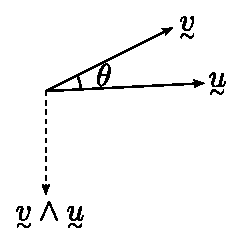
\includegraphics[scale=1.0]{2-7-1.eps}
\caption{Direction of cross product}
\label{Direction of cross product-2-7-1}
\end{figure}

or in determinant form

\begin{equation}
\tenq{v}\wedge\tenq{u}
=
\begin{vmatrix}
\tenq{e}_1 & \tenq{e}_2 & \tenq{e}_3 \\ 
v_1 & v_2 & v_3 \\ 
u_1 & u_2 & u_3
\end{vmatrix}
=
\tenq{e}_1
\begin{vmatrix}
v_2 & v_3 \\ 
u_2 & u_3
\end{vmatrix}
-
\tenq{e}_2
\begin{vmatrix}
v_1 & v_3 \\ 
u_1 & u_3
\end{vmatrix}
+
\tenq{e}_3
\begin{vmatrix}
v_1 & v_2 \\ 
u_1 & u_2
\end{vmatrix}\tag{1}\label{eq: 2-6-(1)}
\end{equation}

Let $X = \left\{ {0;\tenq{e}_1,\tenq{e}_2,\tenq{e}_3} \right\}$ be a rectangular Cartesian coordinate frame with origin $O$ and with unit vector $\tenq{e}_i$.

\begin{framed}
$\mathscr{F}$: the class of all frames\\
$\mathscr{F}_{+}$: the class of all such frames that are also right-handed
\end{framed}

\paragraph{Properties of $\mathscr{F}$ and $\mathscr{F}_+$}\mbox{}\\

if $X \in \mathscr{F} \Rightarrow  \tenq[1]{e}_i \cdot \tenq[1]{e}_j = \delta_{ij}$\\
if $X \in \mathscr{F}_{+} \Rightarrow  \tenq[1]{e}_i \cdot \tenq[1]{e}_j = \delta_{ij}$ and $\left(\tenq[1]{e}_1 \wedge \tenq[1]{e}_2 \right) \cdot \tenq[1]{e}_3 = +1$\\

Let $X\in\mathscr{F}_+$, then the three real numbers defined as
\[u_i^X=\tenq{u}\cdot\tenq{e}_i^X\]

scalar components of vector $\tenq{u}$ on $X$

\begin{note}
No need to put $X$ to the superscript of $\tenq{u}$.
\end{note}

\[\tenq{u}=u_i\tenq{e}_i=u_1\tenq{e}_1+u_2\tenq{e}_2+u_3\tenq{e}_3\]

\begin{align*}
\tenq{u}\cdot\tenq{v}
&= \left(u_i\tenq{e}_i\right)\cdot\left(v_k\tenq{e}_k\right) = u_iv_k\tenq{e}_i\cdot\tenq{e}_k = u_iv_k\delta_{ik} \\
&= u_iv_i=u_kv_k
\end{align*}

\[\therefore\boxed{\tenq{u}\cdot\tenq{v}=u_iv_i}\]

%\begin{align*}
%\Aboxed{\tenq{v}\wedge\tenq{u}
%&\vc{=}{\eqref{eq: 2-6-(1)}}{\eqref{eq: 2-6-*}}\epsilon_{ijk}\tenq{e}_iv_ju_k} \\
%&= \left( \epsilon_{ijk}v_ju_k\right)\tenq{e}_i = \left(\tenq{v}\wedge\tenq{u}\right)_i\tenq{e}_i
%\end{align*}

\begin{equation}
\left.\begin{aligned}
\Aboxed{\tenq{v}\wedge\tenq{u}
&\vc{=}{\eqref{eq: 2-6-(1)}}{\eqref{eq: 2-6-*}}\epsilon_{ijk}\tenq{e}_iv_ju_k} \\
&= \left( \epsilon_{ijk}v_ju_k\right)\tenq{e}_i = \left(\tenq{v}\wedge\tenq{u}\right)_i\tenq{e}_i
\end{aligned}\right. \tag{2}\label{eq: 2-6-(2)}
\end{equation}

\begin{equation}
\therefore\boxed{\left(\tenq{v}\wedge\tenq{u}\right)_i=\epsilon_{ijk}v_ju_k} \tag{3}\label{eq: 2-6-(3)}
\end{equation}

\begin{note}
The expression of equations must be consistent, either in vector form (as \eqref{eq: 2-6-(2)}) or in indicial form (as \eqref{eq: 2-6-(3)}).
\end{note}

\begin{align*}
\left(\tenq{u}\wedge\tenq{v}\right)\cdot\tenq{w}
&= \left(\epsilon_{ijk}u_jv_k\tenq{e}_i\right)\cdot\left(w_l\tenq{e}_l\right) = \epsilon_{ijk}u_jv_kw_l\underbrace{\left(\tenq{e}_{i}\cdot\tenq{e}_l\right)}_{\delta_{il}} \\
&= \epsilon_{ijk}w_iu_jv_k
\end{align*}

If we start with indicial form

\begin{align*}
\left(\tenq{u}\wedge\tenq{v}\right)\cdot\tenq{w}
&= \left(\tenq{u}\wedge\tenq{v}\right)_kw_k = \epsilon_{kij}u_iv_jw_k = \epsilon_{ijk}u_iv_jw_k
\end{align*}

\begin{example}{$\tenq{a}$ and $\tenq{b}$ are any vectors in $E_3$, show that $\left(\tenq{a}\wedge\tenq{b}\right)\cdot\left(\tenq{a}\wedge\tenq{b}\right)+\left(\tenq{a}\cdot\tenq{b}\right)^2=\abs{\tenq{a}}^2\abs{\tenq{b}}^2$.}

\begin{solution}

\begin{align*}
&\left(\tenq{a}\wedge\tenq{b}\right)\cdot\left(\tenq{a}\wedge\tenq{b}\right)+\left(\tenq{a}\cdot\tenq{b}\right)^2 \\
=& \epsilon_{ijk}a_jb_k\epsilon_{ilm}a_lb_m+\left(a_jb_j\right)\left(a_kb_k\right)\\
=& \epsilon_{ijk}\epsilon_{ilm}a_jb_ka_lb_m+a_jb_ja_kb_k \\
=& \left(\delta_{jl}\delta_{km}-\delta_{jm}\delta_{kl}\right)a_jb_ka_lb_m+a_jb_ja_kb_k \\
=& a_jb_ka_jb_k-\cancel{a_jb_ka_kb_j} + \cancel{a_jb_ja_kb_k}\\
=& \abs{\tenq{a}}^2+\abs{\tenq{b}}^2
\end{align*}

\end{solution}

\end{example}

\begin{example}{Show that }

\[
\left(\tenq{a}\wedge\tenq{b}\right)\cdot\left(\tenq{c}\wedge\tenq{d}\right)=
\begin{vmatrix}
\tenq{a}\cdot\tenq{c} & \tenq{b}\cdot\tenq{c} \\ 
\tenq{a}\cdot\tenq{d} & \tenq{b}\cdot\tenq{d}
\end{vmatrix}
\]

\begin{solution}

\begin{align*}
\left(\tenq{a}\wedge\tenq{b}\right)\cdot\left(\tenq{c}\wedge\tenq{d}\right) 
&= \epsilon_{ijk}a_jb_k\epsilon_{ilm}c_ld_m \\
&= \epsilon_{ijk}\epsilon_{ilm}a_jb_kc_ld_m\\
&= \left(\delta_{jl}\delta_{km}-\delta_{jm}\delta_{kl}\right)a_jb_kc_ld_m \\
&= a_jc_jb_kd_k - a_jd_jb_kc_k \\
&= \left(\tenq{a}\cdot\tenq{c}\right)\left(\tenq{b}\cdot\tenq{d}\right)-\left(\tenq{a}\cdot\tenq{d}\right)\left(\tenq{b}\cdot\tenq{c}\right)\\
&= 
\begin{vmatrix}
\tenq{a}\cdot\tenq{c} & \tenq{b}\cdot\tenq{c} \\ 
\tenq{a}\cdot\tenq{d} & \tenq{b}\cdot\tenq{d}
\end{vmatrix}
\end{align*}

\end{solution}

\end{example}




\chapter{Introduction to Cartesian tensor}
\section{Transformation of coordinate frames (Definition of Cartesian tensor)}

Consider two rectangular Cartesian frames 

\begin{align*}
X = \left\{ {0;\tenq{e}_1,\tenq{e}_2,\tenq{e}_3} \right\},
&& 
X' = \left\{ {0;\tenq{e}_1',\tenq{e}_2',\tenq{e}_3'} \right\}
\end{align*} 

\begin{figure}[H]
\centering
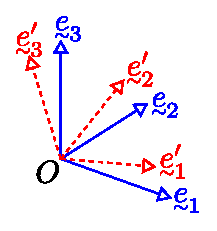
\includegraphics[scale=1.0]{3-1-1.eps}
\caption{Scheme of two rectangular Cartesian frames}
\label{Scheme of two rectangular Cartesian frames-3-1-1}
\end{figure}

Define

\[A_{ij}=\tenq{e}_i'\cdot\tenq{e}_j=\cos(\tenq{e}_i',\tenq{e}_j)=\left(\tenq{e}_i'\right)_j^X=\left(\tenq{e}_j\right)_i^{X'}\]

\[
\tenq{A}=[A_{ij}] = 
\begin{bmatrix}
\tenq{e}_1',\tenq{e}_1 & \tenq{e}_1',\tenq{e}_2 & \tenq{e}_1',\tenq{e}_3 \\ 
\tenq{e}_2',\tenq{e}_1 & \tenq{e}_2',\tenq{e}_2 & \tenq{e}_2',\tenq{e}_3 \\ 
\tenq{e}_3',\tenq{e}_1 & \tenq{e}_3',\tenq{e}_2 & \tenq{e}_3',\tenq{e}_3  
\end{bmatrix}
\]

\[A_{ij}\neq A_{ji}\]

Observed properties 

\[\tenq{e}_p'\cdot\tenq{e}_q'=\delta_{pq}\]

then 

\[A_{pi}A_{qi}=\left(\tenq{e}_p'\right)_i^X\left(\tenq{e}_q'\right)_i^X=\tenq{e}_p'\cdot\tenq{e}_q'\]

\[\Rightarrow \boxed{A_{pi}A_{qi}=\delta_{pq}}\]

Similarly

\[A_{pi}A_{pj}=\left(\tenq{e}_i\right)_p^{X'}\left(\tenq{e}_j\right)_p^{X'}=\tenq{e}_i\cdot\tenq{e}_j\]

\[\Rightarrow \boxed{A_{pi}A_{pj}=\delta_{ij}}\]

in matrix form

\[\tenq{A}\tenq{A}^T=\tenq{A}^T\tenq{A}=\tenq{1}\Rightarrow\tenq{A}=\tenq{A}^{-1}\]

Also

\begin{align*}
\det\tenq{A}
&= \epsilon_{ijk}A_{1i}A_{2j}A_{3k} = \epsilon_{ijk}\left(\tenq{e}_1'\right)_i^X\left(\tenq{e}_2'\right)_j^X\left(\tenq{e}_3'\right)_k^X\\
&= \left(\tenq{e}_1'\wedge\tenq{e}_2'\right)\cdot\tenq{e}_3'
=
\begin{cases}
+1 \text{ right-handed frame}\\
-1 \text{ left-handed frame}
\end{cases}
\end{align*}


\[\therefore\det\tenq{A}=\pm 1\]

$\tenq{A}$ is an \emph{orthogonal} (orthonormal) matrix. \\

If $X\in\mathscr{F}_+$, then $\det\tenq{A}=+1$, $\tenq{A}$ is \emph{proper} matrix.

\begin{notation}\mbox{}\\

The change in coordinate frame $X\to X'$ which is governed by $\tenq{A}$ will be represented as 

\[\tenq{A}\colon X\to X'\]

\end{notation}

Consider a vector $\tenq{v}$

\[\tenq{v}=v_p^X\tenq{e}_p=v_p^{X'}\tenq{e}_p'\]

where 

\begin{align*}
v_p^X &\cdots\text{scalar components of $\tenq{v}$ with respect to frame $X$}\\
v_p^{X'} &\cdots\text{scalar components of $\tenq{v}$ with respect to frame $X'$}
\end{align*}

\[\tenq{v}\cdot\tenq{e}_i'=v_i^{X'}=\left(v_p^X\tenq{e}_p\right)\cdot\tenq{e}_i'=v_p^XA_{ip}\]

\[\Rightarrow\boxed{v_i^{X'}=A_{ip}v_p^X}\]

Similarly

\[\boxed{v_i^X=A_{pi}v_p^{X'}}\]

which are \emph{transformation laws}.

or in matrix form $\tenq{v}=\begin{bmatrix}
v_1^X \\ 
v_2^X\\ 
v_3^X
\end{bmatrix}$\\

$
\left.\begin{aligned}
& \tenq{v}'=\tenq{A}\tenq{v}\\
& \tenq{v}=\tenq{A}^T\tenq{v}'
\end{aligned}\right\}
$ gives confusion, the transformation law only change the \emph{components} of a vector not the vector itself.

\begin{definition}{Definition of vector}\mbox{}\\
A vector is a function defined on all $X$ such that it satisfies the above transformation laws.
\end{definition}

\begin{definition}{Definition of a Cartesian tensor}

Let $N\geq 0$ be an integer. A Cartesian tensor of order $N$ is a function on $\mathscr{F}$ (all $X$) that assigns to each $X\in\mathscr{F}$, an ordered set of $3^N$ real numbers. We will denote

\[V_{\underbrace{ij\cdots k}_{N}}^X\cdots\text{components of $\tenq{V}$ in $X$}\]

such that for every $\tenq{A}\colon X\to X'$ (for every orthogonal transformation which transforms $X$ to $X'$)

\begin{equation}
V_{\underbrace{ij\cdots k}_{N}}^X = A_{ip}A_{jq}\cdots A_{kr}V_{\underbrace{pq\cdots r}_{N}}^X \tag{$\ast$}\label{eq: 3-1-(*)}
\end{equation}

Further, if $\tenq{U}$ and $\tenq{V}$ are both tensors of order $N$ and $c$ is a real number then define

\begin{enumerate}[label=(\roman*)]

\item
$\tenq{U}=\tenq{V}$ if $U_{ij\cdots k}^X=V_{ij\cdots k}^X\phantom{-}\forall X\in\mathscr{F}$

\item \label{ch3-1-def of cart. tensor-(ii)}
$\tenq{W}=\tenq{U}+\tenq{V}$ if $W_{ij\cdots k}^X=U_{ij\cdots k}^X+V_{ij\cdots k}^X\phantom{-}\forall X\in\mathscr{F}$

\item \label{ch3-1-def of cart. tensor-(iii)}
$\tenq{W}=c\tenq{U}$ if $W_{ij\cdots k}^X=cU_{ij\cdots k}^X\phantom{-}\forall X\in\mathscr{F}$

\end{enumerate}

\end{definition}

\begin{note}\mbox{}\\

\begin{enumerate}[label=(\arabic*)]
\item
$V_{ij\cdots k}$ is not a tensor. They are the components of a tensor in a given frame $X$. 

\item
$\tenq{W}$ defined in \ref{ch3-1-def of cart. tensor-(ii)} and \ref{ch3-1-def of cart. tensor-(iii)} is itself a tensor of order $N$.

\item
If $N=0$, $\tenq{V}$ is called a scalar and you write $V$ in place of $\tenq{V}$. 

\item
If $N=1$, $\tenq{V}$ is a vector. 

\item
Equalities needs to be tested for a single frame only.
\end{enumerate}



\end{note}

\begin{definition}\mbox{}\\
A tensor $\tenq{V}$ of order $N\geq 2$ is symmetric/skew symmetric with respect to a pairs of indices of its components if the components of $\tenq{V}$ remain unchanged/change sign under the interchange of these two indices.
\end{definition}


\begin{definition}\mbox{}\\
A tensor is fully symmetric if its is symmetric with respect to any pairs of indices (so as skew symmetric).
\end{definition}


\paragraph{Property}\mbox{}\\

If the component of a tensor are symmetric in one frame then they are symmetric in any other frame

\begin{proof}\mbox{}\\

Let 

\begin{equation}
V_{\cdots i\cdots j\cdots}^X=V_{\cdots j\cdots i\cdots}^X \tag{$\star$}\label{eq: 3-1-star}
\end{equation}

\begin{align*}
V_{\cdots p\cdots q\cdots}^{X'}
&=\cdots A_{pi}\cdots A_{qj}\cdots V_{\cdots i\cdots j\cdots}^X\\
&\vc{=}{\eqref{eq: 3-1-star}}{}{}\cdots A_{qj}\cdots A_{pi}\cdots V_{\cdots j\cdots i\cdots}^X\\
&\vc{=}{\eqref{eq: 3-1-(*)}}{}V_{\cdots q\cdots p\cdots}^{X'}
\end{align*}
\end{proof}

\begin{definition}\mbox{}\\
A tensor $\tenq{V}$ of order $N$ is \emph{isotropic} if its components $V_{ij\cdots k}$ are independents of choice of frame.
\end{definition}

\begin{note}\mbox{}\\

\begin{enumerate}[label=(\arabic*)]

\item
A scalar is an isotropic tensor of order $N=0$. 

\item
The only isotropic vector is the null vector $\tenq{v}=\tenq{0}$.

\end{enumerate}

\end{note}

\begin{claim}\mbox{}\\

\begin{enumerate}[label=(\alph*)]

\item \label{ch3-1-isotropic-claim-(a)}
Let $V_{ij}^X=\delta_{ij}\phantom{-}\footnotemark\forall X\in\mathscr{F}$. $V_{ij}^X$ are the components in frame $X$ of an isotropic second order ($N=2$) tensor. We write $\tenq{V}=\tenq{1}$ (identity tensor).

\item \label{ch3-1-isotropic-claim-(b)}
$V_{ijk}^X=\epsilon_{ijk}\phantom{-}\forall X\in\mathscr{F}_+$. Then $V_{ijk}^X$ are components of an isotropic tensor $\tenq{\epsilon}$ ($N=3$).

\end{enumerate}


\footnotetext{$\forall$, the symbol gives the isotropic property by definition}

\end{claim}

\begin{proof}\mbox{}\\

Sufficient to show that $V_{ij}$ in \ref{ch3-1-isotropic-claim-(a)} and $V_{ij}$ in \ref{ch3-1-isotropic-claim-(b)} are tensor component, i.e. satisfy \eqref{eq: 3-1-(*)}.

\begin{enumerate}[label=(\alph*)]

\item
\[A_{ip}A_{jq}V_{pq}^X=A_{ip}A_{jq}\delta_{ij}=A_{ip}A_{jq}=\delta_{ij}\vc{=}{\text{by}}{\text{def.}}V_{ij}^{X'}\]

\item

\begin{align*}
A_{ip}A_{jq}A_{kr}V_{pqr}^{X}
&=A_{ip}A_{jq}A_{kr}\epsilon_{pqr}=\epsilon_{ijk}\det\tenq{A}\\
&\vc{=}{\footnotemark}{}\epsilon_{ijk} = V_{ijk}^{X'}
\end{align*}



\footnotetext{If $X\in\mathscr{F}_+$, $\det\tenq{A}=+1$}

\end{enumerate}


\end{proof}


From this point on , change notation, denote $\mathscr{F}_+$ by $\mathscr{F}$, i.e. handle only \emph{proper} orthogonal transformation only. 



\begin{claim}\mbox{}\\
\begin{enumerate}[label=(\arabic*)]

\item
Every isotropic tensor of 2\textsuperscript{nd} order is a scalar multiple of $\tenq{1}$. 

\item
Every isotropic tensor of 3\textsuperscript{rd} order is a scalar multiple of $\tenq{\epsilon}$. 

\item
Every isotropic high order tensor can be constructed from $\tenq{1}$ and $\tenq{\epsilon}$. \\
e.g. The most general 4\textsuperscript{th} order isotropic tensor has the form of components

\[C_{ijkl}=\alpha\delta_{ij}\delta_{kl}+\beta\delta_{ik}\delta_{jl}+\gamma\delta_{il}\delta_{jk}\]


where $\alpha$, $\beta$, and $\gamma$ are scalars. 

\end{enumerate}
\end{claim}

\section{Outer multiplication of tensors}

Let $\tenq{U}$ and $\tenq{V}$ be tensor of order $M$ and $N$ respectively. \\

Define 

\[W_{\underbrace{ij\cdots k}_{M}\underbrace{mn\cdots r}_{N}}^X=U_{\underbrace{ij\cdots k}_{M}}^XV_{\underbrace{mn\cdots r}_{N}}^X\phantom{-}\forall X\in\mathscr{F}\]

then $W_{ij\cdots kmn\cdots r}$ are the components of tensor $\tenq{W}$ of order $M+N$ called the outer product of $\tenq{U}$ and $\tenq{V}$ (in that order)

\begin{proof}

\begin{align*}
W_{ij\cdots kmn\cdots r}\vc{=}{\text{by}}{\text{def.}}
&= U_{ij\cdots k}^{X'}V_{mn\cdots r}^{X'} \\
&\vc{=}{\eqref{eq: 3-1-(*)}}{}A_{iI}A_{jJ}\cdots A_{kK}A_{mM}A_{nN}\cdots A_{rR}\underbrace{U_{IJ\cdots K}^XV_{MN\cdots R}^X}_{ 
\vc{=}{\text{by}}{\text{def.}}W_{IJ\cdots KMN\cdots R}^X}
\end{align*}


\end{proof}

\section{Contraction of tensors}

Let $\tenq{U}$ be a tensor of order $N\geq 2$. Let $U_{ij\cdots k}^X$ be its components with $X\in\mathscr{F}$.\\

Define the $3^{N-2}$ real numbers as 

\[V_{\underbrace{ij\cdots k}_{N-2}}^X=U_{\underbrace{ij\cdots r\cdots r\cdots k}_N}^X\phantom{-}X\in\mathscr{F}\]

Then $V_{ij\cdots k}^X$ are components of a new tensor $\tenq{V}$ formed by contraction of $\tenq{U}$.

\begin{proof}\mbox{}\\

Similar to the outer product.

\end{proof}

Let ($N=2$) $U_{ij}^X$ are the components of a 2\textsuperscript{nd} tensor $\tenq{U}$, then 

\[\tenq{V}=U_{rr}^X=U_{11}^X+U_{22}^X+U_{33}^X=\tr \tenq{U}\]

e.g. If $\tenq{U}=\tenq{\sigma}$, the stress tensor, then 

\[\tr \tenq{\sigma}=\sigma_{11}^X+\sigma_{22}^X+\sigma_{33}^X=I_1\]

the 1\textsuperscript{st} invariant of stress tensor.

\section{Operation between tensors}

Let $c$ be a scalar and $\tenq{U}$, $\tenq{V}$ be tensors.\\

Define

\begin{table}[H]
\begin{tabular}{p{4cm}|p{1.2cm}|p{1.2cm}|p{1.2cm}|p{3cm}|p{4cm}}
Definition $\tenq{W}$& order $\tenq{U}$& order $\tenq{V}$& order $\tenq{W}$& Absolute (coordinate-free) notation & Name \\ \hline
$W=U_iV_i$ & 1 & 1 & 0 & $\tenq{W}=\tenq{U}\cdot\tenq{V}$ & dot product betweens two vectors \\ \hline
$W_i=\epsilon_{ijk}U_jV_k$ & 1 & 1 & 1 & $\tenq{W}=\tenq{U}\wedge\tenq{V}$ & cross product \\ \hline
$W_i=U_{ij}V_j$ & 2 & 1 & 1 & $\tenq{W}=\tenq{U}\tenq{V}$ & product \\ \hline
$W_{ijk}=U_{ij}V_k$ & 2 & 1 & 3 & (no notation) & outer product \\ \hline
$W_{ij}=U_{ik}V_{kj}$ & 2 & 2 & 2 & $\tenq{W}=\tenq{U}\tenq{V}$ & 2\textsuperscript{nd} order tensor product \\ \hline
$W_{ij}=U_{i}V_j$ & 1 & 1 & 2 & $\tenq{W}=\tenq{U}\otimes\tenq{V}$ & \emph{Dyadic} or outer product of two vectors \\ \hline
\end{tabular}
\end{table}

\section{Inner product or fully-contracted outer product}


If $\tenq{U}$ and $\tenq{V}$ are both of order $N>0$, define 

\[\tenq{U}\cdot\tenq{V}=U_{ij\cdots k}V_{ij\cdots k}\phantom{-}\]

(no symbol of reference frame needed)\\

Define 

\[\abs{\tenq{U}}=\sqrt{\tenq{U}\cdot\tenq{U}}\]

the \emph{norm} of a tensor $\tenq{U}$.

\begin{claim}{Quotient Rule}

Let 9 real numbers $W_{ij\cdots k}^X$ be defined for all $X\in\mathscr{F}$ (these numbers are not known aprion to be tensor components) and suppose that for any vector $\tenq{u}\neq\tenq{0}$, the 3 real numbers $v_i^X$ defined by 

\begin{align*}
v_i^X=W_{ij}^Xu_j^X
&& 
\forall X\in\mathscr{F}
\end{align*}

are the components in $X$ of a vector $\tenq{v}$. Then $W_{ij}^X$ are components in $X$ of a tensor $\tenq{W}$.

\end{claim}

\begin{proof}\mbox{}\\

By hypothesis, if $\tenq{A}\colon X\to X'$ since both $\tenq{U}$ and $\tenq{V}$ are vectors

\[v_i^X\vc{=}{\eqref{eq: 3-1-(*)}}{}A_{qi}v_q^{X'}\vc{=}{\text{by}}{\text{def.}}W_{ij}^Xu_j^X\vc{=}{\eqref{eq: 3-1-(*)}}{}W_{ij}^X\left(A_{qj}u_q^{X'}\right)\]

multiply by $A_{pi}$

\[
A_{pi}A_{qi}v_q^{X'} = A_{pi}W_{ij}^X A_{qj}u_q^{X'}
\Rightarrow
\delta_{pq}v_q^{X'} = W_{ij}^X A_{pi}A_{qj}u_q^{X'}
\]

\begin{equation}
\Rightarrow
v_p^{X'}=W_{ij}^XA_{pi}A_{qj}u_q^{X'}\tag{1}\label{eq: 3-5-(1)}
\end{equation}

Also by definition


\begin{equation}
v_p^{X'}=W_{pq}^{X'}u_q^{X'}\tag{2}\label{eq: 3-5-(2)}
\end{equation}

\eqref{eq: 3-5-(1)} and \eqref{eq: 3-5-(2)}

\[\left(W_{pq}^{X'}-A_{pi}A_{qj}W_{ij}^X\right)u_q^{X'}=0\]

Choose $\tenq{u}$ such that $u_q^{X'}=\delta_{qs}$ ($s$-fixed)\footnotemark

\footnotetext{choose $\left\{\begin{aligned}
& s=1\to q=1 \\
& s=2\to q=2 \\
& s=3\to q=3 
\end{aligned}\right.$} 

\[\Rightarrow W_{\begin{subarray}{l}
  p1 \\
  \phantom{-}2 \\
  \phantom{-}3
  \end{subarray}}^{X'}-A_{pi}A_{\begin{subarray}{l}
  1j \\
  2\phantom{-} \\
  3\phantom{-}
  \end{subarray}}W_{ij}^X=0\]
  
\[\Rightarrow W_{ps}^{X'}-A_{pi}A_{sj}W_{ij}^X=0\]

i.e. $W_{ij}^X$ obeys transformation law. 



\end{proof}


\section{Product of a second order tensor and a vector}

Let $\tenq{u}$ and $\tenq{v}$ be vectors, $\tenq{W}$ be a 2\textsuperscript{nd} order tensor.\\
Then 

\[\tenq{W}\left(\tenq{u}+\tenq{v}\right)=\tenq{W}\tenq{u}+\tenq{W}\tenq{v}\]

If $X=\left\{0;\tenq{e}_1,\tenq{e}_2,\tenq{e}_3\right\}\in\mathscr{F}$, then 

\[W_{ij}^X=\tenq{e}_i\cdot\left(\tenq{W}\tenq{e}_j\right)\]

the way to find the components of $\tenq{W}$.

\begin{proof}

\begin{align*}
\tenq{e}_i\cdot\left(\tenq{W}\tenq{e}_j\right) 
&= \left(\tenq{e}_i\right)_k\left(\tenq{W}\tenq{e}_j\right)_k = \delta_{ik}\left[W_{kl}\left(\tenq{e}_j\right)_l\right] \\
&= \delta_{ik}W_{kl}\delta_{jl}=W_{ij}
\end{align*}

\end{proof}

\section{Connection between second order tensors and linear vector function (l.v.f.)}

A linear vector function $\tenq{\mathscr{L}}(\bullet)$ is a mapping that assigns to each vector belongs to $E_3$ and other vector $\tenq{v}=\tenq{\mathscr{L}}(\tenq{u})\in E_3$ subjected to the following requirements. 

\begin{enumerate}[label=(\roman*)]

\item
$\tenq{\mathscr{L}}(\tenq{u}^{(1)}+\tenq{u}^{(2)})=\tenq{\mathscr{L}}(\tenq{u}^{(1)})+\tenq{\mathscr{L}}(\tenq{u}^{(2)})$

\item
$\tenq{\mathscr{L}}(c\tenq{u})=c\tenq{\mathscr{L}}(\tenq{u})\phantom{-}\forall c\in\mathbb{R}$

\end{enumerate}

\begin{claim}{Connection of second order tensor to l.v.f.}

\begin{enumerate}[label=(\alph*)]

\item
Let $\tenq{W}$ be a 2\textsuperscript{nd} order tensor and define a function $\tenq{\mathscr{L}}(\bullet)$ as 


\begin{align}
\tenq{v}=\tenq{\mathscr{L}}(\tenq{u}) = \tenq{W}\tenq{u}
&& 
\forall\tenq{u}\in E_3 \tag{$\bigstar$} \label{eq: 3-7-bigstar}
\end{align}

Then $\tenq{\mathscr{L}}$ is a l.v.f.

\item 
Conversely, given a linear vector function $\tenq{\mathscr{L}}(\tenq{u})$, there exists a \emph{unique} 2\textsuperscript{nd} order tensor $\tenq{W}$ such that 

\begin{align*}
\tenq{\mathscr{L}}(\tenq{u}) = \tenq{W}\tenq{u}
&& 
\forall\tenq{u}\in E_3 
\end{align*}

\end{enumerate}

\end{claim}

\begin{proof}\mbox{}\\

\begin{enumerate}[label=(\alph*)]

\item
Recall that $\tenq{W}\left(\tenq{u}+\tenq{v}\right)=\tenq{W}\tenq{u}+\tenq{W}\tenq{v}$

So 

\begin{equation}
\tenq{W}\left(\tenq{u}^{(1)}+\tenq{u}^{(2)}\right)=\tenq{W}\tenq{u}^{(1)} + \tenq{W}\tenq{u}^{(2)} \tag{i} \label{eq: 3-7-i}
\end{equation}

\begin{equation}
\tenq{W}\left(c\tenq{u}\right)=c\tenq{W}\tenq{u} \tag{ii} \label{eq: 3-7-ii}
\end{equation}

\item
Let $\tenq{\mathscr{L}}(\bullet)$ be given. Choose a frame $X=\left\{0;\tenq{e}_1,\tenq{e}_2,\tenq{e}_3\right\}\in\mathscr{F}$. \emph{Let $W_{ji}^X$ be the j\textsuperscript{th} $\tenq{\mathscr{L}}(\tenq{e}_i)$ in frame $X$.}\footnote{Method to find the component of $\tenq{W}$.}

\begin{equation}
\tenq{\mathscr{L}}(\tenq{e}_i)=W_{ji}^X\tenq{e}_j\tag{$\bigstar\bigstar$} \label{eq: 3-7-bigstarbigstar}
\end{equation}

Choose an arbitrary vector $\tenq{u}\in E_3$. Then 

\[\tenq{v}=\tenq{\mathscr{L}}(\tenq{u})=\tenq{\mathscr{L}}(u_i^X\tenq{e}_i)=u_i^X\tenq{\mathscr{L}}(\tenq{e}_i)\vc{=}{\eqref{eq: 3-7-bigstarbigstar}}{}u_i^XW_{ji}^X\tenq{e}_j\]

But $\tenq{v}=v_j^X\tenq{e}_j$

\[\Rightarrow v_j^X=u_i^XW_{ji}^X=W_{ji}^Xu_i^X\vc{=}{i\leftrightarrow j}{}W_{ij}^Xu_j^X\]

By quotient rule, $W_{ij}^X$ are the components of a 2\textsuperscript{nd} order tensor $\tenq{W}$

\[\tenq{v}=\tenq{W}\tenq{u}=\tenq{\mathscr{L}}(\tenq{u})\]

\end{enumerate}

\end{proof}

\paragraph{Uniqueness}\mbox{}\\

Let's assume that exists $\tenq{W}^{(1)}$ and $\tenq{W}^{(2)}$ such that 




\begin{align*}
\left.\begin{aligned}
& \tenq{v}=\tenq{\mathscr{L}}(\tenq{u})= \tenq{W}^{(1)}\tenq{u} \\
& \tenq{v}=\tenq{\mathscr{L}}(\tenq{u})= \tenq{W}^{(2)}\tenq{u} 
\end{aligned}\right\}\Rightarrow\left(\tenq{W}^{(1)}-\tenq{W}^{(2)}\right)\tenq{u}=\tenq{0}
&& 
\forall\tenq{u}\in E_3
\end{align*} 

or 

\[\left(W_{ij}^{(1)}-W_{ij}^{(2)}\right)u_j=0\Rightarrow \tenq{W}^{(1)}=\tenq{W}^{(2)}\]

\begin{note}
Sometimes people define second order tensor by l.v.f.
\end{note}

\section{Transpose of a second order tensor}

Define

\begin{align*}
\tenq{V}=\tenq{U}^T
&& 
\text{if}
&&
V_{ij}=U_{ji}
\end{align*} 

Symmetric 2\textsuperscript{nd} order tensor as one 

\begin{align*}
\tenq{U}=\tenq{U}^T
&& 
\text{or}
&&
U_{ij}=U_{ji}
\end{align*} 

Skew-symmetric 2\textsuperscript{nd} order tensor as one 

\begin{align*}
\tenq{U}=-\tenq{U}^T
&& 
\text{or}
&&
U_{ij}=-U_{ji}
\end{align*} 


If $\tenq{W}$ is a 2\textsuperscript{nd} order tensor and $\tenq{u}$, $\tenq{v}$ are vectors, then 

\[\boxed{\tenq{u}\cdot\left(\tenq{W}\tenq{v}\right)=\left(\tenq{W}^T\tenq{u}\right)\cdot\tenq{v}}\]

\begin{proof}

\begin{align*}
\tenq{u}\cdot\left(\tenq{W}\tenq{v}\right) 
&= u_i\left(\tenq{W}\tenq{v}\right)_i = u_i\left(W_{ij}v_j\right) \vc{=}{i\leftrightarrow j}{}\left(W_{ji}u_j\right)v_i \\
&= \left(\tenq{W}^T\tenq{u}\right)_iv_i = \left(\tenq{W}^T\tenq{u}\right)\cdot\tenq{v}
\end{align*}

\end{proof}

If $\tenq{y}=\tenq{V}\tenq{x}$, $\tenq{z}=\tenq{U}\tenq{y}$ ($\tenq{x},\tenq{y},\tenq{z}\in E_3$, $\tenq{U},\tenq{V}$ are 2\textsuperscript{nd} order tensors)

\begin{align*}
\tenq{z}=\tenq{U}\tenq{V}\tenq{x}
&& 
\text{or}
&&
z_i=U_{ij}V_{jk}x_k
\end{align*} 

\section{Product between two second order tensors}

If $\tenq{U}$ and $\tenq{V}$ are 2\textsuperscript{nd} order tensors, then define 

\begin{align*}
\tenq{W}=\tenq{U}\tenq{V}
&& 
\text{if}
&&
W_{ij}=U_{ik}V_{kj}
\end{align*}

as tensorial product of $\tenq{U}$ and $\tenq{V}$.

\begin{enumerate}[label=(\roman*)]

\item
distribute

\[\tenq{U}\left(\tenq{V}^{(1)}+\tenq{V}^{(2)}\right)=\tenq{U}\tenq{V}^{(1)}+\tenq{U}\tenq{V}^{(2)}\]

\item
associate

\[\left(\tenq{U}\tenq{V}\right)\tenq{W}=\tenq{U}\left(\tenq{V}\tenq{W}\right)\]

\item
non-commutative

\[\tenq{U}\tenq{V}\neq\tenq{V}\tenq{U}\]

\end{enumerate}

If $\tenq{W}=\tenq{U}\tenq{V}$, then 

\[\tenq{W}^T=\tenq{V}^T\tenq{U}^T\]

\begin{proof}

\begin{align*}
W_{ij}=U_{ik}V_{kj} \vc{\Rightarrow}{i\leftrightarrow j}{}W_{ji}
&= U_{jk}V_{ki} \\
&= V_{ki}U_{jk} \\
&= V_{ik}^TU_{kj}^T \\
&= \left(\tenq{V}^T\tenq{U}^T\right)_{ij}
\end{align*}

but $W_{ji}=W_{ij}^T$

\[\therefore\tenq{W}^T=\tenq{V}^T\tenq{U}^T\]

\end{proof}

\section{Tensor (or dyadic) product between two vectors}

If $\tenq{u}$ and $\tenq{v}$ belong to $E_3$, define

\begin{align*}
\tenq{W}=\tenq{u}\otimes \tenq{v}
&& 
\text{if}
&&
W_{ij}=u_{i}v_{j}
\end{align*}

where $\tenq{W}$ is a 2\textsuperscript{nd} order tensor.

\begin{note}\mbox{}\\

\begin{enumerate}[label=(\arabic*)]

\item
\[\tenq{u}\otimes\tenq{v}\neq\tenq{v}\otimes\tenq{u}\]

\item
\[\tenq{u}\otimes\left(\tenq{v}^{(1)}+\tenq{v}^{(2)}\right)=\tenq{u}\otimes\tenq{v}^{(1)} + \tenq{u}\otimes\tenq{v}^{(2)}\]

\item
\[\tenq{W}=\tenq{u}\otimes\tenq{v}\Leftrightarrow\tenq{W}\tenq{a}=\left(\tenq{v}\cdot\tenq{a}\right)\tenq{u}\phantom{-}\forall \tenq{a}\in E_3\]

\end{enumerate}

\begin{proof}\mbox{}\\

\paragraph{$\boxed{\Rightarrow}$}

\[
\tenq{W}\tenq{a}
= \left(W_{ik}a_k\right)\tenq{e}_i = \left(u_iv_ka_k\right)\tenq{e}_i = \left(v_ka_k\right)u_i\tenq{e}_i=\left(\tenq{v}\cdot\tenq{a}\right)\tenq{u}
\]

\paragraph{$\boxed{\Leftarrow}$}

\begin{align*}
\tenq{W}\tenq{a}=\left(\tenq{v}\cdot\tenq{a}\right)\tenq{u}
&& 
\forall\tenq{a}\in E_3
\end{align*}

or 

\[W_{ij}a_j=v_ja_ju_i\]

\[\therefore\left(W_{ij}-u_iv_j\right)a_j=0\]

Since $\tenq{a}$ is arbitrary 

\begin{align*}
W_{ij}=u_iv_j
&& 
\text{or}
&&
\tenq{W}=\tenq{u}\otimes\tenq{v}
\end{align*}


\end{proof}

\end{note}

If $X=\left\{0;\tenq{e}_1,\tenq{e}_2,\tenq{e}_3\right\}\in\mathscr{F}$, then 

\[\boxed{\tenq{W}=W_{ij}^X\tenq{e}_i\otimes\tenq{e}_j}\]

\begin{proof}

\[\tenq{V}=W_{ij}^X\tenq{e}_i\otimes\tenq{e}_j=W_{11}\tenq{e}_1\otimes\tenq{e}_1+W_{12}\tenq{e}_1\otimes\tenq{e}_2+\cdots\]

\begin{align*}
V_{pq}=\left(W_{ij}^X\tenq{e}_i\otimes\tenq{e}_j\right)_{pq}
&= W_{ij}^X\left(\tenq{e}_i\otimes\tenq{e}_j\right)_{pq} \\
&= W_{ij}^X\left(\tenq{e}_i\right)_p\left(\tenq{e}_j\right)_q\\
&= W_{ij}^X\delta_{ip}\delta_{jq} \\
&= W_{pq}^X
\end{align*}

\[\therefore \left(W_{ij}^X\tenq{e}_i\otimes\tenq{e}_j\right)_{pq}=W_{pq}^X\]

or 

\[W_{ij}^X\tenq{e}_i\otimes\tenq{e}_j=\tenq{W}\]

representation theorem of $\tenq{W}$ in terms of a sum of unit vectors of a frame admits components in the same frame.\\

Trace of a 2\textsuperscript{nd} order tensor $\tenq{U}$ as 

\[\tr \tenq{U}=U_{ii}=U_{11}+U_{22}+U_{33}\]

Let $\tenq{U}$ and $\tenq{V}$ be 2\textsuperscript{nd} order tensors, then 

\begin{enumerate}[label=(\arabic*)]

\item
\[\tenq{U}\cdot\tenq{V}=U_{ij}V_{ij}=\tr (\tenq{U}\tenq{V}^T)\]

\item
\[\abs{\tenq{U}}=\sqrt{\tenq{U}\cdot\tenq{U}}=\sqrt{\tr (\tenq{U}\tenq{U}^T)}\]

\item \label{ch3-10-(3)}
\[\det(\tenq{U}\tenq{V})=\det\tenq{U}\det\tenq{V}\]

\begin{proof}
exercise
\end{proof}

\end{enumerate}


\end{proof}

\section{Orthogonal tensors}

A 2\textsuperscript{nd} order tensor $\tenq{Q}$ is orthogonal if $\tenq{Q}\tenq{Q}^T=\tenq{1}$, the identity tensor.

\[\underbrace{\tenq{Q}^{-1}\tenq{Q}}_{\tenq{1}}\tenq{Q}^T=\tenq{Q}^{-1}\Rightarrow\tenq{Q}^T=\tenq{Q}^{-1}\]

or 

\[\det(\tenq{Q}\tenq{Q}^{T})=\det\tenq{1}=1\vc{=}{\ref{ch3-10-(3)}}{}\det\tenq{Q}\det\tenq{Q}^T=\left(\det\tenq{Q}\right)^2\]

\[\Rightarrow\det\tenq{Q}=\pm 1\]

If $\tenq{Q}\tenq{Q}^{T}=\tenq{1}$ and $\det\tenq{Q}=+1$, then $\tenq{Q}$ is called \emph{proper orthogonal}.

\section{Fundamental scalar invariant of a second order tensor}

Let $\tenq{V}$ be a 2\textsuperscript{nd} order tensor. Then define $I_i(\tenq{V})$ as 

\begin{align*}
& I_1(\tenq{V}) = \tr \tenq{V}=V_{ii}=V_{11}+V_{22}+V_{33} \\
& I_2(\tenq{V}) = \frac{1}{2}\left(V_{ii}V_{jj}-V_{ij}V_{ij}\right)=\frac{1}{2}\left[\left(\tr \tenq{V}\right)^2-\tr \tenq{V}^2\right]\\
& I_3(\tenq{V}) = \frac{1}{6}\epsilon_{ijk}\epsilon_{pqr}V_{ip}V_{jq}V_{kr}=\det\tenq{V}
\end{align*}

$I_i(\tenq{V})$ are scalars produced by outer multiplication and contraction and as such as scalars independent of frame.

\begin{definition}\mbox{}\\
A 2\textsuperscript{nd} order tensor $\tenq{V}$ is non-singular if $\det\tenq{V}\neq 0$; otherwise, a 2\textsuperscript{nd} order tensor $\tenq{V}$ is singular if there exists a vector $\tenq{u}\neq \tenq{0}$ such that $\tenq{V}\tenq{u}=\tenq{0}$ or $V_{ij}u_j=0$, then by Cramer's rule $\det[V_{ij}]=0$.
\end{definition}

\begin{claim}\mbox{}\\

\begin{enumerate}[label=(\alph*)]

\item
Let $X=\left\{0;\tenq{e}_1,\tenq{e}_2,\tenq{e}_3\right\}\in\mathscr{F}$. Also let $\tenq{Q}$ be a proper orthogonal tensor and define vectors $\tenq{e}_i'=\tenq{Q}\tenq{e}_i$. Then vector trait $\tenq{e}_i'$ are base vectors for an other proper orthogonal frame $X'=\left\{0;\tenq{e}_1',\tenq{e}_2',\tenq{e}_3'\right\}\in\mathscr{F}$ and the matrix $\tenq{A}$ of direction cosines that transforms $X$ to $X'$ ($\tenq{A}\colon X\to X'$) is given by $A_{ij}=Q_{ji}^X$. 

\item
Let $X=\left\{0;\tenq{e}_1,\tenq{e}_2,\tenq{e}_3\right\}\in\mathscr{F}$ and $X'=\left\{0;\tenq{e}_1',\tenq{e}_2',\tenq{e}_3'\right\}\in\mathscr{F}$ and also let $\tenq{A}\colon X\to X'$ then there exists an \emph{unique} (proper orthogonal) such that $\tenq{e}_i'=\tenq{Q}\tenq{e}_i$ and $\tenq{Q}$ is determined by $Q_{ij}^X=A_{ji}$. 

\end{enumerate}

\end{claim}

\begin{proof}\mbox{}\\

\[\tenq{e}_i'\cdot\tenq{e}_j'=\left(\tenq{Q}\tenq{e}_i\right)\cdot\left(\tenq{Q}\tenq{e}_j\right)\vc{=}{\footnotemark}{}\underbrace{\tenq{Q}^T\tenq{Q}}_{\tenq{1}}\underbrace{\tenq{e}_i\cdot\tenq{e}_j}_{\delta_{ij}}=\delta_{ij}\]

\footnotetext{$\tenq{u}\cdot\left(\tenq{W}\tenq{v}\right)=\left(\tenq{W}^T\tenq{u}\right)\cdot\tenq{v}$}

By definition of $\tenq{A}$

\[\tenq{e}_i'\cdot\tenq{e}_j=A_{ij}\]

\[\therefore A_{ij}=\tenq{e}_i'\cdot\tenq{e}_j=\left(\tenq{Q}\tenq{e}_i\right)\cdot\tenq{e}_j\vc{=}{\footnotemark}{}Q_{ji}^X\]

\footnotetext{$W_{ij}^X=\tenq{e}_i\cdot\left(\tenq{W}\tenq{e}_j\right)$}

\[\det\tenq{A}=\det\tenq{Q}^T=\det\tenq{Q}=+1\]

\end{proof}

\section{Principal value and principal direction of second order tensors definition}

Let $\tenq{V}$ be a second order tensor, a real number $\lambda=\lambda(\tenq{V})$ is a principal value (or an eigenvalue) of $\tenq{V}$ if there exists a vector $\tenq{n}$ such that

\begin{align*}
\tenq{V}\tenq{n}=\lambda\tenq{n}
&& 
\text{and}
&&
\tenq{n}\cdot\tenq{n}=1
\end{align*} 

or 

\begin{align*}
V_{ij}n_j=\lambda n_i
&& 
\text{and}
&&
n_in_i=1
\end{align*} 


If so, $\tenq{n}$ is called a principal direction (or eigenvector) of $\tenq{V}$ corresponding to eigenvalue $\lambda$

\begin{enumerate}

\item

\begin{figure}[H]
\centering
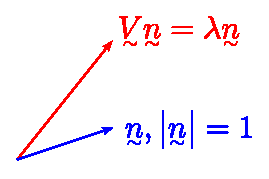
\includegraphics[scale=1.0]{3-13-1-(1).eps}
\caption{Scheme of non-principal direction vector}
\label{Scheme of non-principal direction vector-3-13-1-(1)}
\end{figure}

if $\tenq{n}$ is \emph{not} a principal direction vector.

\item

\begin{figure}[H]
\centering
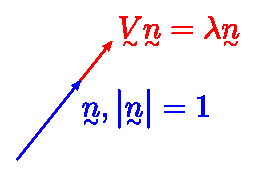
\includegraphics[scale=1.0]{3-13-1-(2).eps}
\caption{Scheme of principal direction vector}
\label{Scheme of principal direction vector-3-13-1-(2)}
\end{figure}

if $\tenq{n}$ is a principal direction vector.


\end{enumerate}

Also $\tenq{n}$ and $-\tenq{n}$ define a principal direction or principal axis belonging to eigenvalue $\lambda$. 


\begin{claim}\mbox{}\\
Let $\tenq{V}$ be a 2\textsuperscript{nd} order tensor. Then $\lambda$ is a principal value of $\tenq{V}$ if and only if it is a real root of the cubic equation

\[F(\lambda)=\det(\tenq{V}-\lambda\tenq{1})=-\lambda^3+I_1(\tenq{V})\lambda^2-I_2(\tenq{V})\lambda+I_3(\tenq{V})=0\]

which is characteristic equation of $\tenq{V}$. \\

If $\lambda$ is a principal value of $\tenq{V}$, then the principal direction vector belonging to $\lambda$ are the solutions for $\tenq{n}$ of the equations

\[
\left\{\begin{aligned}
& \left(V_{ij}-\lambda\delta_{ij}\right)n_j=0 \\
& n_in_i=1
\end{aligned}\right.
\]

\begin{note}
Every 2\textsuperscript{nd} order tensor has at least one real eigenvalue (since a cubic of real coefficient has at least one real root). If the other roots are complex, they are complex conjugate. 
\end{note}


\begin{proof}\mbox{}\\

Let $\lambda$ be eigenvalue, then there exists 3 real numbers $n_i$, not all zeros such that

\[V_{ij}n_j-\lambda n_i=0\]

or 

\[\left(V_{ij}-\lambda\delta_{ij}\right)n_j=0\]

From Cramer's Rule

\[\det(V_{ij}-\lambda\delta_{ij})=0\]

(for non-trivial solution)

\[\det(V_{ij}-\lambda\delta_{ij})=\frac{1}{6}\epsilon_{ijk}\epsilon_{pqr}\left(V_{ip}-\lambda\delta_{ip}\right)\left(V_{jq}-\lambda\delta_{jq}\right)\left(V_{kr}-\lambda\delta_{kr}\right)=0\]

(by definition of invariants)

\[\Rightarrow -\lambda^3+I_1(\tenq{V})\lambda^2-I_2(\tenq{V})\lambda+I_3(\tenq{V})=0\]

\end{proof}

\end{claim}

\section{Symmetric tensors for second order tensors}

\begin{theorem}\label{ch3-14-thm.}\mbox{}\\

Let $\tenq{V}=\tenq{V}^T$, then all three roots ($\lambda_1,\lambda_2,\lambda_2$) of the characteristic equation are real. 

\begin{equation}
F(\lambda)=\det(\tenq{V}-\lambda\tenq{1})=-\lambda^3+I_1\lambda^2-I_2\lambda+I_3=0 \tag{i}\label{eq: 3-14-(i)}
\end{equation}

Further, there exists \emph{at least} one set of three mutually perpendicular principal axes of $\tenq{V}$ and if $X'=\left\{0;\tenq{e}_1',\tenq{e}_2',\tenq{e}_3'\right\}\in\mathscr{F}$ is a principal frame for $\tenq{V}$ then one has

\begin{align*}
[V_{ij}^{X'}]
=
\begin{bmatrix}
\lambda_1 & 0 & 0 \\ 
0 & \lambda_2 & 0 \\ 
0 & 0 & \lambda_3  
\end{bmatrix}
&& 
\text{or}
&&
V_{ij}^{X'}=\lambda_i\delta_{ij}\phantom{-}\text{(no sum)}
\end{align*} 

provided that

\begin{align*}
\tenq{V}\tenq{e}_i'=\lambda_i\tenq{e}_i'
&& 
\text{(no sum)}
\end{align*} 

i.e. $\tenq{e}_i'$ are principal direction vectors.


\begin{enumerate}[label= \fbox{Case \Roman*}]

\item
($\lambda_1,\lambda_2,\lambda_3$) are distinct roots of \eqref{eq: 3-14-(i)} (simple roots) then there exists a unique principal axis belonging to each principal value $\lambda_i$ and the three principal axes are mutually perpendicular. 

\item
Say $\lambda_1\neq\lambda_2=\lambda_3=\lambda_\ast$, i.e. \eqref{eq: 3-14-(i)} has one simple root and a double root. Then there exists a unique principal axis belonging to $\lambda_1$ and every axis which is perpendicular to the former is a principal axis belonging to $\lambda_\ast$. 

\item
$\lambda_1=\lambda_2=\lambda_3=\lambda_\ast$, i.e. \eqref{eq: 3-14-(i)} has a triple root. Then every axis is a principal axis belonging to $\lambda_\ast$ and 

\begin{align*}
\tenq{V}=\lambda_\ast\tenq{1}
&& 
\text{or}
&&
V_{ij}=\lambda_\ast\delta_{ij}
&&
\forall X\in\mathscr{F}
\end{align*} 

so $\tenq{V}$ is an isotropic tensor. 


\end{enumerate}


\end{theorem}

\begin{lemma}\label{ch3-14-lemma 1}\mbox{}\\

If $\tenq{n}^{(1)}$ and $\tenq{n}^{(2)}$ are principal direction vectors belonging to two \emph{distinct} principal values $\lambda_1$ and $\lambda_2$, then $\tenq{n}^{(1)}\perp\tenq{n}^{(2)}$. 

\end{lemma}

\begin{proof}\mbox{}\\

\begin{equation}
\left\{\begin{aligned}
& \tenq{V}\tenq{n}^{(1)}=\lambda_1\tenq{n}^{(1)} \\
& \tenq{V}\tenq{n}^{(2)}=\lambda_2\tenq{n}^{(2)}
\end{aligned}\right.\text{ where }\tenq{V}=\tenq{V}^T\tag{$\circledS$}\label{eq: 3-14-circledS}
\end{equation}

\begin{align*}
\tenq{n}^{(2)}\cdot\lambda_1\tenq{n}^{(1)}
&\vc{=}{\eqref{eq: 3-14-circledS}}{}\tenq{n}^{(2)}\cdot\tenq{V}\tenq{n}^{(1)}\vc{=}{\footnotemark}{}\left(\tenq{V}^T\tenq{n}^{(2)}\right)\cdot\tenq{n}^{(1)}\\
&\vc{=}{\tenq{V}^T=\tenq{V}}{}\tenq{V}\tenq{n}^{(2)}\cdot\tenq{n}^{(1)}\vc{=}{\eqref{eq: 3-14-circledS}}{}\lambda_2\tenq{n}^{(2)}\cdot\tenq{n}^{(1)}
\end{align*}


\footnotetext{$\tenq{u}\cdot\left(\tenq{W}\tenq{v}\right)=\left(\tenq{W}^T\tenq{u}\right)\cdot\tenq{v}$}

\[\Rightarrow\left(\lambda_1-\lambda_2\right)\tenq{n}^{(2)}\cdot\tenq{n}^{(1)}=0\]

\[\vc{\Rightarrow}{\lambda_1\neq\lambda_2}{}\tenq{n}^{(2)}\cdot\tenq{n}^{(1)}=0\text{ or }\tenq{n}^{(2)}\perp\tenq{n}^{(1)}\]

\end{proof}

\begin{lemma}\label{ch3-14-lemma 2}\mbox{}\\

Let $\lambda$ be a principal value of a symmetric, 2\textsuperscript{nd} order tensor $\tenq{V}$ and $\tenq{n}$ be a principal vector belonging to $\lambda$. For fixed $k$ ($k=1,2,3$), choose $X=\left\{0;\tenq{e}_1,\tenq{e}_2,\tenq{e}_3\right\}\in\mathscr{F}$ in such a way that $\tenq{e}_k=\tenq{n}$, i.e. $\tenq{V}\tenq{n}=\lambda\tenq{n},\tenq{V}\tenq{e}_k=\lambda\tenq{e}_k$. Then 

\[V_{ki}^X=V_{ik}^X=\lambda\delta_{ik}\]

e.g. $k=1$

\[V_{ki}^X
=
\begin{bmatrix}
\lambda & 0 & 0 \\ 
0 & V_{22}^X & V_{23}^X \\ 
0 & V_{32}^X & V_{33}^X  
\end{bmatrix}
\]

\end{lemma}

\begin{proof}\mbox{}\\

Choose and fix $k$. By hypothesis

\[\tenq{V}\tenq{e}_k=\lambda\tenq{e}_k\Rightarrow V_{ij}^X\left(\tenq{e}_k\right)_j=\lambda\left(\tenq{e}_k\right)_i\Rightarrow V_{ij}^X\delta_{kj}=\lambda\delta_{ki}\]

\[\Rightarrow V_{ki}^X=\lambda\delta_{ki}\]

\end{proof}

\begin{proof}{Proof of theorem \ref{ch3-14-thm.}}

Let $\tenq{n}^{(1)}$ be a principal direction vector belonging to $\lambda_1$. Choose frame $X'=\left\{0;\tenq{e}_1',\tenq{e}_2',\tenq{e}_3'\right\}\in\mathscr{F}$ that $\tenq{e}_1'=\tenq{n}^{(1)}$. Then by lemma \ref{ch3-14-lemma 2} 

\begin{align}
\tenq{V}_{1i}^{X'}=\lambda_1\delta_{i1}
&& 
\text{or}
&&
V_{11}^{X'}=\lambda_1,V_{12}^{X'}=V_{21}^{X'}=V_{13}^{X'}=V_{31}^{X'}=0
\tag{a}\label{eq: 3-14-pf.-a}
\end{align} 

Thus 

\[\det(V_{ij}^{X'}-\lambda\delta_{ij})=\det
\begin{bmatrix}
\lambda_1-\lambda & 0 & 0 \\ 
0 & V_{22}^{X'}-\lambda &  V_{23}^{X'}-\lambda \\ 
0 & V_{32}^{X'}-\lambda &  V_{33}^{X'}-\lambda  
\end{bmatrix}=0
\]

\begin{equation}
\Rightarrow\left(\lambda_1-\lambda\right)\left\{\lambda^2-\left(V_{22}^{X'}+V_{33}^{X'}\right)\lambda+V_{22}^{X'}V_{33}^{X'}-\left(V_{23}^{X'}\right)^2\right\}=0\tag{b}\label{eq: 3-14-pf.-b}
\end{equation}



\begin{equation}
\left.\begin{aligned}
 \therefore \lambda&=\lambda_1 \\
 \lambda&=
\begin{pmatrix}
\lambda_2 \\
\lambda_3 
\end{pmatrix}\\
&=\frac{V_{22}^{X'}+V_{33}^{X'}}{2}\\
&\pm\underbrace{\sqrt{\frac{\left(V_{22}^{X'}+V_{33}^{X'}\right)-4\left[V_{22}^{X'}V_{33}^{X'}-\left(V_{23}^{X'}\right)^2\right]}{4}}}_{\sqrt{\frac{\left(V_{22}^{X'}-V_{33}^{X'}\right)^2}{4}+\left(V_{23}^{X'}\right)^2}}
\end{aligned}\right.\tag{c}\label{eq: 3-14-pf.-c}
\end{equation}

the roots are real roots.

\begin{enumerate}[label= \fbox{Case \Roman*}]

\item $\lambda_1,\lambda_2,\lambda_3$ are distinct\\

Let $\tenq{n}^{(i)}$ be the three principal axes belonging to $\lambda_i$ by lemma \ref{ch3-14-lemma 1}, $\tenq{n}^{(i)}$ are mutually perpendicular. Let $X'=\left\{0;\tenq{e}_1',\tenq{e}_2',\tenq{e}_3'\right\}\in\mathscr{F}$ such that $\tenq{n}^{(1)}=\tenq{e}_1'$, $\tenq{n}^{(2)}=\tenq{e}_2'$, $\tenq{n}^{(3)}=\tenq{e}_3'$. By lemma \ref{ch3-14-lemma 2} for $k=1,2,3$

\begin{align*}
\left.\begin{aligned}
& V_{i1}^{X'}=\lambda_1\delta_{i1}\\
& V_{i2}^{X'}=\lambda_2\delta_{i2}\\
& V_{i3}^{X'}=\lambda_3\delta_{i3}
\end{aligned}\right\}V_{ij}^{X'}=\lambda_j\delta_{ij}
&&
\text{(no sum)}
\end{align*}

i.e.

\[[V_{ij}^{X'}]=
\begin{bmatrix}
\lambda_1 & 0 & 0 \\ 
0 & \lambda_2 & 0 \\ 
0 & 0 & \lambda_3  
\end{bmatrix}
\]

\item $\lambda_1\neq\lambda_2=\lambda_3=\lambda_\ast$\\

Choose $X'=\left\{0;\tenq{e}_1',\tenq{e}_2',\tenq{e}_3'\right\}\in\mathscr{F}$ such that $\tenq{e}_1'=\tenq{n}^{(1)}$ then \eqref{eq: 3-14-pf.-a} holds, i.e. $V_{11}^{X'}=\lambda_1$, $V_{12}^{X'}=V_{21}^{X'}=V_{13}^{X'}=V_{31}^{X'}=0$. In addition, $\lambda_2=\lambda_3=\lambda_\ast$

\begin{equation}
\vc{\Rightarrow}{\eqref{eq: 3-14-pf.-c}}{}V_{22}^{X'}=V_{33}^{X'}=\lambda_\ast,V_{23}^{X'}=V_{32}^{X'}=0 \tag{d}\label{eq: 3-14-pf.-d}
\end{equation}

i.e. 

\[[V_{ij}^{X'}]=
\begin{bmatrix}
\lambda_1 & 0 & 0 \\ 
0 & \lambda_\ast & 0 \\ 
0 & 0 & \lambda_\ast  
\end{bmatrix}
\]

To show that any choice of $\tenq{e}_2'$, $\tenq{e}_3'$ ($\perp\tenq{n}^{(1)}$) is principal axis

\[\left(\tenq{V}\tenq{e}_2'\right)_i=V_{ij}^{X'}\left(\tenq{e}_2'\right)_j=V_{ij}^{X'}\delta_{2j}=V_{i2}^{X'}=\lambda_\ast\delta_{i2}=\lambda_\ast\left(\tenq{e}_2'\right)_i\]

\[\therefore \tenq{V}\tenq{e}_2'=\lambda_\ast\tenq{e}_2'\]

Similarly

\[
\tenq{V}\tenq{e}_3'=\lambda_\ast\tenq{e}_3'
\]

\begin{figure}[H]
\centering
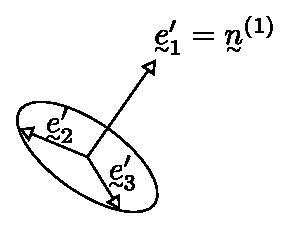
\includegraphics[scale=1.0]{3-14-1.eps}
\caption{Scheme of eigenvectors of $\lambda_1\neq\lambda_2=\lambda_3=\lambda_\ast$}
\label{Scheme of eigenvectors of l1,l2,l3-3-14-1}
\end{figure}

infinite choice of $\tenq{e}_2'$ and $\tenq{e}_3'$. 

\item $\lambda_1=\lambda_2=\lambda_3=\lambda_\ast$\\
Choose $X'=\left\{0;\tenq{e}_1',\tenq{e}_2',\tenq{e}_3'\right\}\in\mathscr{F}$ such that $\tenq{e}_1'=\tenq{n}^{(1)}$ (one eigenvector belonging to $\lambda_1=\lambda_\ast$). Then \eqref{eq: 3-14-pf.-a} holds and \eqref{eq: 3-14-pf.-d} holds, i.e. 

\begin{align*}
[V_{ij}^{X'}]=
\begin{bmatrix}
\lambda_\ast & 0 & 0 \\ 
0 & \lambda_\ast & 0 \\ 
0 & 0 & \lambda_\ast  
\end{bmatrix}
&&
\text{or}
&&
V_{ij}^{X'}=\lambda_\ast\delta_{ij}
&&
\text{or}
&&
\tenq{V}=\lambda_\ast\tenq{1}
\end{align*}

\[\Rightarrow\tenq{V}\tenq{n}=\lambda_\ast\tenq{1}\tenq{n}=\lambda_\ast\tenq{n}\]

where $\tenq{n}$ is any unit vector vector. \\

Every unit vector $\tenq{n}$ is a principal direction vector belonging to $\lambda_\ast$ and every frame $X\in\mathscr{F}$ is a principal frame for $\tenq{V}$. 


\end{enumerate}



\end{proof}

\begin{theorem}{Spectral Representation theorem}

Let $X' = \left\{ {0;\tenq{e}_1',\tenq{e}_2',\tenq{e}_3'} \right\}\in\mathscr{F}$ is a principal frame for a symmetric 2\textsuperscript{nd} tensor $\tenq{V}$ and let $\lambda_i$ be the eigenvectors. Then 

\[\tenq{V}=\sum_{i=1}^3\lambda_i\tenq{e}_i'\otimes\tenq{e}_i'=\lambda_1\tenq{e}_1'\otimes\tenq{e}_1'+\lambda_2\tenq{e}_2'\otimes\tenq{e}_2'+\lambda_3\tenq{e}_3'\otimes\tenq{e}_3'\]

\end{theorem}

\begin{proof}\mbox{}\\

Recall that for all $X\in\mathscr{F}$, not necessary principal

\[\tenq{V}=V_{ij}^X\tenq{e}_i\otimes\tenq{e}_j\]

if we choose a principal frame $X' = \left\{ {0;\tenq{e}_1',\tenq{e}_2',\tenq{e}_3'} \right\}\in\mathscr{F}$, then $V_{ij}^{X'}=\lambda_i\delta_{ij}\phantom{-}\text{(no sum)}$\\

So 

\begin{align*}
\tenq{V}
&= V_{11}^{X'}\tenq{e}_1'\otimes\tenq{e}_1'+V_{12}^{X'}\tenq{e}_1'\otimes\tenq{e}_2'+V_{13}^{X'}\tenq{e}_1'\otimes\tenq{e}_3'+\cdots \\
&= \lambda_1\tenq{e}_1'\otimes\tenq{e}_1'+0+0+\cdots \\
&= \lambda_1\tenq{e}_1'\otimes\tenq{e}_1'+\lambda_2\tenq{e}_2'\otimes\tenq{e}_2'+\lambda_3\tenq{e}_3'\otimes\tenq{e}_3'
\end{align*}

\end{proof}

If $\lambda_1\neq\lambda_2=\lambda_3=\lambda_\ast$, then 

\[\tenq{V}=\left(\lambda_1-\lambda_\ast\right)\tenq{e}_1'\otimes\tenq{e}_1'+\lambda_\ast\tenq{1}\footnotemark\]

\footnotetext{$\displaystyle\because\tenq{1}=\sum_{j=1}^3\tenq{e}_j'\otimes\tenq{e}_j'$ (Homework)}

If $\lambda_1=\lambda_2=\lambda_3=\lambda_\ast$, then 

\[\tenq{V}\lambda_\ast\tenq{1}\]


\section{Skew-symmetric tensors for second order tensors}

\begin{align*}
\tenq{V}=-\tenq{V}^T
&& 
\text{or}
&&
V_{ij}=-V_{ji}
\end{align*} 

\[[V_{ij}]=
\begin{bmatrix}
0 & V_{12} & V_{13} \\ 
-V_{12} & 0 & V_{23} \\ 
-V_{13} & -V_{23} & 0  
\end{bmatrix}\Rightarrow\det\tenq{V}=0
\]

every skew-symmetric tensor is \emph{singular}. \\

Three number $V_{12}$, $V_{13}$, $V_{23}$ are needed to define a skew symmetric tensor. \\

Define a vector $\tenq{w}$ as follows

\begin{align}
\tenq{w}=\textit{dual }\tenq{V}
&& 
\text{if}
&&
w_i=\frac{1}{2}\epsilon_{ijk}V_{kj}\tag{$\star$} \label{eq: 3-15-star}
\end{align} 

The component $V_{ij}$ of $\tenq{V}$ are related to $\tenq{w}$ by 

\begin{align*}
V_{ij}=\epsilon_{ikj}w_k
&& 
\text{or}
&&
[V_{ij}]=
\begin{bmatrix}
0 & -\omega_3 & -\omega_2 \\ 
\omega_3 & 0 & -\omega_1 \\ 
\omega_2 & \omega_1 & 0  
\end{bmatrix}
\end{align*} 

\begin{proof}\mbox{}\\

From \eqref{eq: 3-15-star}

\[w_i=\frac{1}{2}\epsilon_{ijk}V_{kj}\]

multiply both side by $-\epsilon_{ipq}$

\begin{align*}
-\epsilon_{ipq}w_i 
&= -\frac{1}{2}\epsilon_{ipq}\epsilon_{ijk}V_{kj} \\
&= -\frac{1}{2}\left(\delta_{pj}\delta_{qk}-\delta_{pk}\delta_{qj}\right)V_{kj} \\
&= -\frac{1}{2}\left(V_{qp}-V_{pq}\right)=V_{pq}
\end{align*}

\[\therefore V_{pq}=\epsilon_{piq}w_i\vc{\Rightarrow}{i\to k}{\begin{subarray}{l}
  p\to i \\
  q\to j
  \end{subarray}}V_{ij}=\epsilon_{ikj}w_k\]
  
\end{proof}
  
If $\tenq{V}$ is skew-symmetric and $\tenq{w}=\textit{dual }\tenq{V}$, then 

\[\boxed{\tenq{V}\tenq{u}=\tenq{w}\wedge\tenq{u}\phantom{-}\forall\tenq{u}\in E_3}\]

\begin{proof}\mbox{}\\

\[\left(\tenq{w}\wedge\tenq{u}\right)_i=\underbrace{\epsilon_{ikj}w_k}_{V_{ij}}u_j = V_{ij}u_j=\left(\tenq{V}\tenq{u}\right)_i\]



\end{proof}

\section{Decomposition Theorem for second order tensors}

\begin{claim}\mbox{}\\
Every 2\textsuperscript{nd} order tensor $\tenq{W}$ admits a \emph{unique} decomposition such that

\begin{equation}
\tenq{W}=\tenq{U}+\tenq{V}\tag{$\ast$}\label{eq: 3-15-*}
\end{equation}

where 

\begin{alignat*}{3}
& \tenq{U}     \quad && \colon\text{symmetric } \quad && (\tenq{U}=\tenq{U}^T)\\
& \tenq{V}     \quad && \colon\text{skew-symmetric } \quad && (\tenq{V}=-\tenq{V}^T)
\end{alignat*}



Further this resolution is 

\begin{equation}
\left\{\begin{aligned}
& \tenq{U}=\frac{1}{2}\left(\tenq{W}+\tenq{W}^T\right) \\
& \tenq{V}=\frac{1}{2}\left(\tenq{W}-\tenq{W}^T\right) 
\end{aligned}\right.\tag{$\ast\ast$}\label{eq: 3-15-**}
\end{equation}

or 

\[
\left\{\begin{aligned}
& U_{ij}=\frac{1}{2}\left(W_{ij}+W_{ji}\right) \\
& V_{ij}=\frac{1}{2}\left(W_{ij}-W_{ji}\right) 
\end{aligned}\right.
\]

\begin{align*}
\tenq{U}=\textit{sym }\tenq{W}
&& 
\tenq{V}=\textit{skew }\tenq{W}
\end{align*}



\end{claim}

\begin{claim}{Isotropic tensors of 1\textsuperscript{st} and 2\textsuperscript{nd} order tensor}

\begin{enumerate}[label=(\alph*)]

\item\label{ch3-16-claim-(a)}
If $\tenq{v}$ is an isotropic vector, then $\tenq{v}=\tenq{0}$. 
\item\label{ch3-16-claim-(b)}
If $\tenq{V}$ is an isotropic \emph{skew-symmetric} 2\textsuperscript{nd} order tensor, then $\tenq{V}=\tenq{0}$.
\item
If $\tenq{V}$ is an isotropic 2\textsuperscript{nd} order tensor, then $\tenq{V}=\alpha\tenq{1}$, $\alpha\in\mathbb{R}$. 

\end{enumerate}

\end{claim}

\begin{proof}\mbox{}\\

\begin{enumerate}[label=(\alph*)]

\item
$\tenq{v}$ is an isotropic vector, choose $X=\left\{0;\tenq{e}_1,\tenq{e}_2,\tenq{e}_3\right\}\in\mathscr{F}$, $\tenq{v}=v_i^X\tenq{e}_i$. Construct $X'=\left\{0;\tenq{e}_1',\tenq{e}_2',\tenq{e}_3'\right\}=\left\{0;\tenq{e}_1,\tenq{e}_3,-\tenq{e}_2\right\}$.

\begin{figure}[H]
\centering
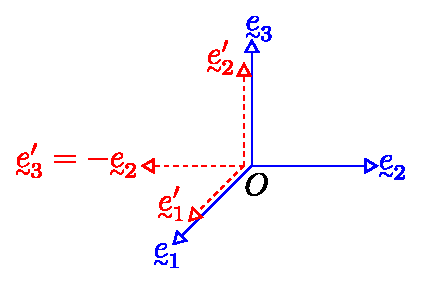
\includegraphics[scale=1.0]{3-16-1.eps}
\caption{Scheme of frame $X'$}
\label{Scheme of frame Xp-3-16-1}
\end{figure}

$X'$ obtained from $X$ by rotation about $\tenq{e}_1$ axis (angle: $\pi/2$)\\

Define $X''=\left\{0;\tenq{e}_1'',\tenq{e}_2'',\tenq{e}_3''\right\}\in\mathscr{F}$ by rotation of $X$ through $\pi/2$ about $\tenq{e}_1$ axis, i.e. $X''=\left\{0;\tenq{e}_1'',\tenq{e}_2'',\tenq{e}_3''\right\}=\left\{0;-\tenq{e}_3,\tenq{e}_2,\tenq{e}_1\right\}$.\\

By the definition of isotropic tensor

\[
\begin{bmatrix}
v_1 \\ 
v_2 \\ 
v_3  
\end{bmatrix}_{X}
=
\begin{bmatrix}
\tenq{v}\cdot\tenq{e}_1'=\tenq{v}\cdot\tenq{e}_1= v_1 \\ 
\tenq{v}\cdot\tenq{e}_2'=\tenq{v}\cdot\tenq{e}_3= v_3 \\ 
\tenq{v}\cdot\tenq{e}_3'=\tenq{v}\cdot\left(-\tenq{e}_2\right)= -v_2  
\end{bmatrix}_{X'}
=
\begin{bmatrix}
-v_3 \\ 
v_2 \\ 
v_1  
\end{bmatrix}_{X''}
\]

\[\Rightarrow
\left\{\begin{aligned}
& v_1=-v_3 \\
& v_3=v_2 \\
& -v_2=v_1 
\end{aligned}\right.\]

\[\Rightarrow v_1=v_2=v_3=0\]

\item
Let $\tenq{V}=-\tenq{V}^T$ and be isotropic

\[\tenq{w}=\textit{dual }\tenq{V}\]

or 

\[w_i=\frac{1}{2}\underbrace{\epsilon_{ijk}}_{\text{isotropic}} \underbrace{V_{kj}}_{\begin{subarray}{l}
  \text{isotropic} \\
  \text{by hypothesis}
  \end{subarray}}\Rightarrow\tenq{w}\text{ is isotropic}\vc{=}{\ref{ch3-16-claim-(a)}}{}\tenq{w}=0 \]
  
\[\Rightarrow\tenq{V}=\tenq{0}\]

\item
Let $\tenq{V}\neq 0$ be an isotropic tensor, then both $\textit{sym }\tenq{V}$ and $\textit{skew }\tenq{V}$ are isotropic. By \ref{ch3-16-claim-(b)} $\textit{skew }\tenq{V}=\tenq{0}$, thus 


\begin{align*}
\tenq{V}=\textit{sym }\tenq{V}
&& 
\text{or}
&&
\tenq{V}=\tenq{V}^T
\end{align*} 

i.e. any non-zero isotropic tensor is symmetric. \\

Thus there exists a frame $X=\left\{0;\tenq{e}_1,\tenq{e}_2,\tenq{e}_3\right\}\in\mathscr{F}$ such that

\begin{align*}
[V_{ij}^X]
=
\begin{bmatrix}
\lambda_1 & 0 & 0 \\ 
0 & \lambda_2 & 0 \\ 
0 & 0 & \lambda_3  
\end{bmatrix}
&& 
\text{and}
&&
\tenq{V}\tenq{e}_i=\lambda_i\tenq{e}_i\phantom{-}\text{(no sum)}
\end{align*} 

Introduce $X'=\left\{0;\tenq{e}_1',\tenq{e}_2',\tenq{e}_3'\right\}=\left\{0;\tenq{e}_2,\tenq{e}_3,\tenq{e}_1\right\}\in\mathscr{F}$

\begin{align*}
V_{ij}^{X'}
&=\tenq{e}_i'\cdot\left(\tenq{V}\tenq{e}_j'\right)\\
&\vc{=}{\text{spectral}}{\text{representation thm.}}\tenq{e}_i'\cdot\left(\lambda_1\tenq{e}_1\otimes\tenq{e}_1+\lambda_2\tenq{e}_2\otimes\tenq{e}_2+\lambda_3\tenq{e}_3\otimes\tenq{e}_3\right)\tenq{e}_j'
\end{align*}

\[\because\tenq{e}_1'=\tenq{e}_2,\tenq{e}_2'=\tenq{e}_3,\tenq{e}_3'=\tenq{e}_1\]

\begin{align*}
V_{11}^{X'}
&= \tenq{e}_1'\cdot\left(\lambda_1\tenq{e}_1\otimes\tenq{e}_1+\lambda_2\tenq{e}_2\otimes\tenq{e}_2+\lambda_3\tenq{e}_3\otimes\tenq{e}_3\right)\tenq{e}_1'\\
&= \tenq{e}_2\cdot\left(\lambda_1\tenq{e}_1\otimes\tenq{e}_1+\lambda_2\tenq{e}_2\otimes\tenq{e}_2+\lambda_3\tenq{e}_3\otimes\tenq{e}_3\right)\tenq{e}_2\\
&\vc{=}{\footnotemark}{}\tenq{e}_2\cdot\left[\lambda_1\tenq{e}_1\left(\tenq{e}_1\cdot\tenq{e}_2\right)+\lambda_2\tenq{e}_2\left(\tenq{e}_2\cdot\tenq{e}_2\right)+\lambda_3\tenq{e}_3\left(\tenq{e}_3\cdot\tenq{e}_2\right)\right]\\
&= \lambda_2
\end{align*}

\footnotetext{$\left(\tenq{u}\otimes\tenq{v}\right)\tenq{a}=\left(\tenq{v}\cdot\tenq{a}\right)\tenq{u}$}

Similarly

\begin{align*}
V_{22}^{x'}=\lambda_3,
&& 
V_{33}^{X'}=\lambda_1
&&
\text{and}
&&
V_{ij}^{X'}=0,i\neq j
\end{align*} 

\[\therefore [V_{ij}^{X'}]=
\begin{bmatrix}
\lambda_2 & 0 & 0 \\ 
0 & \lambda_3 & 0 \\ 
0 & 0 & \lambda_1  
\end{bmatrix}\vc{\Longrightarrow}{\text{isotropic}}{[V_{ij}^X]=[V_{ij}^{X'}]}\lambda_1=\lambda_2,\lambda_2=\lambda_3,\lambda_3=\lambda_1
\]

i.e. $\lambda_1=\lambda_2=\lambda_3=\alpha$ or $\tenq{V}=\alpha\tenq{1}$. 

\end{enumerate}

\end{proof}

\begin{claim}\mbox{}\\

Every 2\textsuperscript{nd} order tensor $\tenq{W}$ admits a unique additive decomposition such that

\begin{equation}
\tenq{W}=\tenq{U}+\tenq{V}\tag{$\ast$}\label{eq: 3-16-*}
\end{equation}

where 

\begin{align*}
\tr\tenq{U}=0,
&&
\tenq{V}\text{ is isotropic}
\end{align*}

The resolution is given by 

\begin{align*}
\tenq{V}=\frac{1}{3}\left(\tr\tenq{W}\right)\tenq{1},
&&
\tenq{U}=\tenq{W}-\tenq{V}=\tenq{W}-\frac{1}{3}\left(\tr\tenq{W}\right)\tenq{1}
\end{align*}

or in component form

\begin{align}
V_{ij}=\frac{1}{3}W_{kk}\delta_{ij},
&&
U_{ij}=W_{ij}-\frac{1}{3}W_{kk}\delta_{ij} \tag{$\ast\ast$}\label{eq: 3-16-**}
\end{align}

\end{claim}

\begin{proof}\mbox{}\\

Assume the existence of the decomposition \eqref{eq: 3-16-*}, then 

\begin{align*}
\tenq{U}=\tenq{W}-\tenq{V}
&&
\text{and}
&&
\tenq{V}=\alpha\tenq{1}\text{ ($\because\tenq{V}$ is isotropic)}
\end{align*}

\[\Rightarrow \tr\tenq{W}=\tr\tenq{U}+\tr\tenq{V}=0+\alpha\tr\tenq{1}=3\alpha\]

\[\Rightarrow\alpha=\frac{1}{3}\tr\tenq{W}\]

or 

\[\tenq{V}=\frac{1}{3}\left(\tr\tenq{W}\right)\tenq{1}\]

\[\tenq{U}=\tenq{W}-\frac{1}{3}\left(\tr\tenq{W}\right)\tenq{1}\]

$\tenq{U}$ is called deviatoric (or traceless) part of $\tenq{W}$.\\

$\tenq{V}$ is called the hydrostatic (or spherical) or isotropic part of $\tenq{W}$. 

\end{proof}

\begin{lemma}{Square root of positive definite symmetric 2\textsuperscript{nd} order tensor}

\begin{definition}\mbox{}\\
$\tenq{S}$ is \emph{positive definite} if $\tenq{v}\cdot\left(\tenq{S}\tenq{v}\right)>0$ $\forall\tenq{v}\in E_3$, $\tenq{v}\neq 0$.
\end{definition}

Let $\tenq{S}$ be a symmetric, positive definite 2\textsuperscript{nd} order tensor. Then there exists a \emph{unique}, \emph{symmetric}, positive definite 2\textsuperscript{nd} order tensor $\tenq{U}$ such that 


\begin{align*}
\tenq{U}\tenq{U}=\tenq{U}^2=\tenq{S}
&& 
\text{or}
&&
U_{ik}U_{kj}=S_{ij}
\end{align*}

One calls $\tenq{U}$ the square root of $\tenq{S}$ and denote $\tenq{U}=\sqrt{\tenq{S}}$. One can show that if $\lambda_i$ are the eigenvalues of $\tenq{S}$, then $\lambda_i>0$, and $\alpha_i=\sqrt{\lambda_i}$ are the eigenvalue of $\tenq{U}=\sqrt{\tenq{S}}$, i.e. if $X'=\left\{0;\tenq{e}_1',\tenq{e}_2',\tenq{e}_3'\right\}\in\mathscr{F}$ is the principal frame for $\tenq{S}$, the $X'$ is also principal frame for $\tenq{U}=\sqrt{\tenq{S}}$ and 

\begin{align*}
[S_{ij}^{X'}]=
\begin{bmatrix}
\lambda_1 & 0 & 0 \\ 
0 & \lambda_2 & 0 \\ 
0 & 0 & \lambda_3  
\end{bmatrix},
&&
[U_{ij}^{X'}]=
\begin{bmatrix}
\sqrt{\lambda_1} & 0 & 0 \\ 
0 & \sqrt{\lambda_2} & 0 \\ 
0 & 0 & \sqrt{\lambda_3}  
\end{bmatrix}
\end{align*}


\end{lemma}

\begin{proof}\mbox{}\\

$\tenq{S}$ is symmetric so there exists $X'=\left\{0;\tenq{e}_1',\tenq{e}_2',\tenq{e}_3'\right\}\in\mathscr{F}$ such that

\[
[S_{ij}^{X'}]=
\begin{bmatrix}
\lambda_1 & 0 & 0 \\ 
0 & \lambda_2 & 0 \\ 
0 & 0 & \lambda_3  
\end{bmatrix}
\]

Let $\tenq{v}=\tenq{e}_1'$, since $\tenq{S}$ is positive definite, i.e. $\tenq{e}_1\cdot\left(\tenq{S}\tenq{e}_1'\right)>0$

\[\Rightarrow S_{11}^{X'}>0\Rightarrow\lambda_1>0\]

Similarly, let $\tenq{v}=\tenq{e}_2'$

\[\Rightarrow\lambda_2>0\]

and 

\[\tenq{v}=\tenq{e}_3'\Rightarrow\lambda_3>0\]

Now construct a symmetric 2\textsuperscript{nd} order tensor $\tenq{U}$ such that $\tenq{U}$ has the same principal frame as $\tenq{S}$, i.e. $X'$, and in that form

\begin{equation}
[U_{ij}^{X'}]
=
\begin{bmatrix}
\sqrt{\lambda_1} & 0 & 0 \\ 
0 & \sqrt{\lambda_2} & 0 \\ 
0 & 0 & \sqrt{\lambda_3}  
\end{bmatrix}
=
\begin{bmatrix}
\alpha_1 & 0 & 0 \\ 
0 & \alpha_2 & 0 \\ 
0 & 0 & \alpha_3  
\end{bmatrix};\alpha_i=\sqrt{\lambda_i}>0\tag{$\circledS$}\label{eq: 3-16-circledS}
\end{equation}

The $\tenq{U}$ constructed this way satisfies

\[\tenq{U}\tenq{U}=\tenq{S}\]

and $\tenq{U}$ is positive definite and symmetric $\Rightarrow$ identified \emph{one} square root of $\tenq{S}$.\\

One has to show now that $\tenq{U}$ given by \eqref{eq: 3-16-circledS} is \emph{unique}. \\
\begin{framed}
If $\tenq{S}\tenq{e}=\tenq{U}^2\tenq{e}=\mu\tenq{e}$, $\abs{\tenq{e}}=1$, $\mu>0$, then we can prove $\tenq{U}\tenq{e}=\sqrt{\mu}\tenq{e}$ where $\tenq{e}$ is a principal direction vector of $\tenq{S}$. 
\end{framed}


\[\Rightarrow\left(\tenq{U}^2-\mu\tenq{1}\right)\tenq{e}=\tenq{0}\]

\[\Rightarrow\left(\tenq{U}+\sqrt{\mu}\tenq{1}\right)\underbrace{\left(\tenq{U}-\sqrt{\mu}\tenq{1}\right)\tenq{e}}_{\equiv \tenq{v}}=\tenq{0}\]

Assume $\tenq{v}\neq 0$, then 

\begin{align*}
\left(\tenq{U}+\sqrt{\mu}\tenq{1}\right)\tenq{v}=\tenq{0}
&\Rightarrow\tenq{U}\tenq{v}=-\sqrt{\mu}\tenq{v}\\
&\Rightarrow\tenq{v}\cdot\left(\tenq{U}\tenq{v}\right)=-\sqrt{\mu}\left(\tenq{v}\cdot\tenq{v}\right)<0
\end{align*}

which contradicts the assumption that $\tenq{U}$ is positive definite. So 

\[\tenq{v}=\tenq{0}\Rightarrow\tenq{U}\tenq{e}=\sqrt{\mu}\tenq{e}\]

\end{proof}


\begin{theorem}{Polar decomposition}

Let $\tenq{W}$ be a non-singular 2\textsuperscript{nd} order tensor ($\det\tenq{W}\neq 0$). Then there exists unique 2\textsuperscript{nd} order tensor $\tenq{U}$, $\tenq{V}$, $\tenq{Q}$, and $\tenq{Q}'$ such that

\begin{equation}
\left\{\begin{aligned}
& \tenq{W}=\tenq{Q}\tenq{U}=\tenq{V}\tenq{Q}'\footnotemark \\
& \tenq{Q},\tenq{Q}'\colon\text{orthogonal},\tenq{U},\tenq{V}\colon\text{symmetric definite}
\end{aligned}\right.\tag{$\ast$}\label{eq: 3-16-polar-*}
\end{equation}

\footnotetext{$\tenq{Q}\tenq{U}\colon$ right decomposition, $\tenq{V}\tenq{Q}'\colon$ left decomposition.}

and

\begin{align*}
\tenq{U}=\sqrt{\tenq{W}^T\tenq{W}},
&&
\tenq{V}=\sqrt{\tenq{W}\tenq{W}^T}
\end{align*}

\begin{align*}
\tenq{Q}=\tenq{W}\tenq{U}^{-1},
&&
\tenq{Q}'=\tenq{V}^{-1}\tenq{W}
\end{align*}

Further

\begin{align*}
\tenq{Q}=\tenq{Q}',
&&
\tenq{V}=\tenq{Q}\tenq{U}\tenq{Q}^T
&&
\tenq{U}=\tenq{Q}^T\tenq{V}\tenq{Q}
\end{align*}

If in addition $\det\tenq{W} >0$, then $\tenq{Q}$ is \emph{proper} orthogonal, i.e. $\det\tenq{Q}=+1$. 



\end{theorem}

\begin{proof}\mbox{}\\

\begin{enumerate}

\item
If $\tenq{Q}=\tenq{Q}'$, then \eqref{eq: 3-16-polar-*} $\Rightarrow\tenq{V}=\tenq{Q}\tenq{U}\tenq{Q}^T$, $\tenq{U}=\tenq{Q}^T\tenq{V}\tenq{Q}$.

\item
Concentrate existence and uniqueness of right decomposition, i.e. 

\[\tenq{W}=\tenq{Q}\tenq{U}\]

Assume that there exists $\tenq{Q}$ and $\tenq{U}$ such that

\begin{equation}
\tenq{W}=\tenq{Q}\tenq{U}, \tenq{Q}\tenq{Q}^T=\tenq{1}, \tenq{U}^T=\tenq{U},\tenq{U}\colon\text{positive definite}\tag{1}\label{eq: 3-16-polar-pf-(1)}
\end{equation} 

Let 

\begin{align}
\tenq{S}=\tenq{W}^T\tenq{W},
&& 
S_{ij}=W_{ki}W_{kj}\tag{2}\label{eq: 3-16-polar-pf-(2)}
\end{align} 

\[\tenq{S}=\tenq{U}^T\underbrace{\tenq{Q}^T\tenq{Q}}_{\tenq{1}}\tenq{U}=\tenq{U}^T\tenq{U}=\tenq{U}\tenq{U}=\tenq{U}^2\]

So

\begin{equation}
\tenq{S}=\tenq{S}^T \tag{3}\label{eq: 3-16-polar-pf-(3)}
\end{equation}

\begin{equation}
\eqref{eq: 3-16-polar-pf-(2)}\&\eqref{eq: 3-16-polar-pf-(3)}\Rightarrow\tenq{U}=\sqrt{\tenq{W}^T\tenq{W}} \tag{4}\label{eq: 3-16-polar-pf-(4)}
\end{equation}

\begin{equation}
\text{From \eqref{eq: 3-16-polar-pf-(1)}},\tenq{Q}=\tenq{W}\tenq{U}^{-1} \tag{5}\label{eq: 3-16-polar-pf-(5)}
\end{equation}

Now need to prove that $\tenq{U}=\sqrt{\tenq{W}^T\tenq{W}}$ is meaningful, i.e. $\tenq{S}=\tenq{W}^T\tenq{W}$ is symmetric and positive definite and $\tenq{Q}$ from \eqref{eq: 3-16-polar-pf-(5)} is orthogonal. 

\[\because\tenq{S}=\tenq{W}^T\tenq{W}\]

\[\Rightarrow\tenq{S}^T=\left(\tenq{W}^T\tenq{W}\right)^T=\tenq{W}^T\left(\tenq{W}^T\right)^T=\tenq{W}^T\tenq{W}=\tenq{S}\]

Also, $\det\tenq{S}=\det\tenq{W}^T\det\tenq{W}=\left(\det\tenq{W}\right)^2>0$ ($\because\det\tenq{W}\neq 0$)

\begin{align*}
\tenq{x}\cdot\tenq{S}\tenq{x}
&= \tenq{x}\cdot\left(\tenq{W}^T\tenq{W}\right)\tenq{x}=\tenq{x}\cdot\tenq{W}^T\left(\tenq{W}\tenq{x}\right) \\
&\vc{=}{\footnotemark}{}\left(\tenq{W}\tenq{x}\right)\cdot\left(\tenq{W}\tenq{x}\right)>0
\end{align*}

\footnotetext{$\tenq{u}\cdot\left(\tenq{F}\tenq{v}\right)=\left(\tenq{F}^T\tenq{u}\right)\cdot\tenq{v}$}

Then $\tenq{S}$ is symmetric and positive definite. \\

From \eqref{eq: 3-16-polar-pf-(5)}, $\tenq{Q}=\tenq{W}\tenq{U}^{-1}$

\begin{align*}
\tenq{Q}\tenq{Q}^T=\tenq{W}\tenq{U}^{-1}\underbrace{\left(\tenq{U}^{-1}\right)^T}_{\left(\tenq{U}^{T}\right)^{-1}}\tenq{W}^T
&= \tenq{W}\left(\tenq{U}^T\tenq{U}\right)^{-1}\tenq{W}^T \\
&= \tenq{W}\underbrace{\left(\tenq{U}^2\right)^{-1}}_{\tenq{S}^{-1}}\tenq{W}^T\\
&= \tenq{W}\left(\tenq{W}^T\tenq{W}\right)^{-1}\tenq{W}^T\\
&= \tenq{W}\tenq{W}^{-1}\left(\tenq{W}^{T}\right)^{-1}\tenq{W}^T\\
&= \tenq{1}
\end{align*}

\item
The left decomposition proof is left as exercise. 

\item
Let $\det\tenq{W}>0\Rightarrow\det\tenq{W}\vc{=}{\eqref{eq: 3-16-polar-*}}{}\det\tenq{Q}\det\tenq{U}>0$. From the fact $\tenq{U}=\sqrt{\tenq{S}}$, $\tenq{S}$ is symmetric positive definite

\[\therefore\det\tenq{U}>0\Rightarrow\det\tenq{Q}>0\]

\[\Rightarrow\det\tenq{Q}=+1\text{, i.e. $\tenq{Q}$ is proper orthogonal}\]

\end{enumerate}

\end{proof}



\chapter{Tensor Calculus}

Let $S \in E_3$ be a point set. A tensor field of order $N$ on $S$ is an $N$-th order tensor valued function of position defined on $S$. Before the next section, we need to review some concepts in vector calculus in appendix \ref{appendix: Some definitions concerning curves, surfaces, and regions}.
\section{Smoothness of tensor fields}
Let $R$ be a region in $E_3$. Let $\tenq{V}$ be a tensor field of order $N$ on $R$. $\tenq{V}$ is continuous on $R$ and we will write $\tenq{V} \in C(R)$ if the functions $V_{\underbrace{ij \cdots k}_{N}}^{X}$ are continuous scalar functions on $R$ $\forall X \in \mathscr{F}$. We say that $\tenq{V}$ is $M$ times continuously differentiable on $R$ ($M$ is positive integer) and write $\tenq{V} \in C^M(R)$ if $\tenq{V} \in C(R)$ and the partial derivatives $\frac{{{\partial ^M}V_{ij \cdots k}^X}}{{\underbrace {\partial {x_p}\partial {x_q} \cdots \partial {x_r}}_M}} = V_{\underbrace {ij \cdots k}_N,\underbrace {pq \cdots r}_M}^X$ exist on $\mathring{R}$ $\forall X \in \mathscr{F}$ and they coincide with continuous function. 

\begin{theorem}
Let $R$ be a domain (open region) and $\tenq{V} \in C^M(R)$ $(M \geq 1)$ be a tensor field of order $N$.\\
Define 

\[W_{ij \cdots ks}^X(\tenq{x}) = \frac{\partial }{{\partial {x_s}}}\left\{ {V_{ij \cdots k}^X(\tenq{x})} \right\},\forall \tenq{x} \in R,\forall X \in \mathscr{F}\]

where $x_s$ are the coordinates in $X$ of points in $R$. 

\begin{figure}[H]
\centering
\input{figure1.eps_tex}
\caption{Scheme for $R$}
\label{Scheme for $R$}
\end{figure}


Then $W_{ij \cdots ks}^X$ are the $3^{N+1}$ components in $X$ of a tensor field $\tenq{W}$ of order $N+1$ and $\tenq{W} \in C^{M-1}(R)$.\\
One calls $\tenq{W}$ the \emph{gradient} of $\tenq{V}$ and writes
\[\tenq{W} = \textit{grad }\tenq{V}=\nabla \tenq{V}\] 
Also
\[W_{ij \cdots ks}^X = V_{ij \cdots k,s}^X \footnote{partial derivative with respect to $x_s$}\]

\begin{proof}\mbox{}\\
Consider $X = \left\{ {0;\tenq{e}_1,\tenq{e}_2,\tenq{e}_3} \right\} \in \mathscr{F}$, $X' = \left\{ {0;\tenq{e'}_1,\tenq{e'}_2,\tenq{e'}_3} \right\} \in \mathscr{F}$ and the matrix $\tenq{A}$ of direction cosine that transforms $X$ to $X'$ $(\tenq{A}\colon X \to X')$.
\[
\begin{cases}
\tenq{x} = x_i\tenq{e}_i = x'_m\tenq{e'}_m\\
x'_m = A_{mi}x_i, x_i = A_{mi}x'_m
\end{cases}
\]

\begin{align*}
W_{pq \cdots rs}^{X'}(\tenq{x}) 
&= \frac{\partial }{{\partial {x'_s}}}\left\{ {V_{pq \cdots r}^{X'}(\tenq{x})} \right\} 
= \frac{\partial }{{\partial {x'_s}}}\left\{A_{pi}A_{qj} \cdots A_{rk} {V_{ij \cdots k}^{X}(\tenq{x})} \right\} \\
&= \frac{\partial }{{\partial {x_l}}}\left\{A_{pi}A_{qj} \cdots A_{rk} {V_{ij \cdots k}^{X}(\tenq{x})} \right\}\frac{{\partial {x_l}}}{{\partial {x'_s}}}
\end{align*}

where 
\[\frac{{\partial {x_l}}}{{\partial {{x'}_s}}} = \frac{{\partial \left( {{A_{ml}}{{x'}_m}} \right)}}{{\partial {{x'}_s}}} = {A_{ml}}\frac{{\partial {{x'}_m}}}{{\partial {{x'}_s}}} = {A_{ml}}{\delta _{ms}} = {A_{sl}}\] \nonumber

\begin{align*}
\therefore W_{pq \cdots rs}^{X'}(\tenq{x}) 
&= A_{pi}A_{qj} \cdots A_{rk}A_{sl}\frac{\partial }{{\partial {x_l}}}\left\{ {V_{pq \cdots r}^{X}(\tenq{x})} \right\}\\
&= A_{pi}A_{qj} \cdots A_{rk}A_{sl} W_{ij \cdots kl}^{X}(\tenq{x})
\end{align*}
satisfies the transformation law
\end{proof}

\end{theorem}

\section{Relation to vector calculus}

Let $R$ be a domain. Let $\phi$ and $\tenq{v}$ be suitably smooth scalar and vector field respectively. \\

Define

%\begin{align*}
%\tenq{W} &= \textit{grad }\phi \equiv \nabla\phi \textit{ if } w_i = \phi_{,i} = \frac{\partial \phi}{\partial x_i}\\
%\psi &= \textit{div }\phi \equiv \nabla\cdot\tenq{V} \textit{ if } \psi = v_{i,i} = \frac{\partial v_i}{\partial x_i}\\
%\end{align*}

\begin{alignat*}{4}
&\tenq{w} &=   &\textit{grad }\phi          &\quad\equiv &  \nabla\phi  & \quad \textit{ if }w_i &= \phi_{,i}  = \frac{\partial \phi}{\partial x_i}\\
&\psi  &= &\textit{div }\tenq{v}          &\quad\equiv &   \nabla\cdot\tenq{v} &\quad \textit{ if }\psi &= v_{i,i} = \frac{\partial v_i}{\partial x_i}\\
&\tenq{w}  &= &\textit{curl }\tenq{v}          &\quad\equiv &   \nabla\wedge\tenq{v} &\quad \textit{ if } w_i &= \epsilon_{ijk}\frac{\partial}{\partial x_j}v_k = \epsilon_{ijk}v_{k,j}\\
&\psi  &= &\textit{Lap }\phi          &\quad\equiv &   \nabla^2\phi  &\quad \textit{ if } w_i &= \phi_{,ii} = \frac{\partial^2\phi}{\partial x_1^2} + \frac{\partial^2\phi}{\partial x_2^2} + \frac{\partial^2\phi}{\partial x_3^2}\\
&\tenq{w}  &= &\textit{Lap }\tenq{v}          &\quad\equiv &   \nabla^2\tenq{v}  &\quad \textit{ if } w_i &= v_{i,kk}\\ 
\end{alignat*}

\begin{notation}\mbox{}\\
\begin{itemize}
\item $\nabla \phi \neq \phi_{,i}$ but ${\left( {\nabla \phi } \right)_i} = {\phi _{,i}}$ or $\nabla \phi  = {\phi _{,i}}\tenq{e}_i$
\item $\nabla^2\tenq{v} = v_{i,kk}\tenq{e}_i$
\end{itemize}
\end{notation}



\begin{example}
$\tenq{u} \in C^1(R)$ is a vector field. Show that
\[\tenq{u} \wedge \left( {\nabla  \wedge \tenq{u}} \right) = \frac{1}{2}\nabla \left( {\tenq{u} \cdot \tenq{u}} \right) - \left( {\tenq{u} \cdot \nabla } \right)\tenq{u}\]
which is important relation for continuum mechanics.
\end{example}

\begin{proof}
\begin{align*}
{\left[ \tenq{u} \wedge \left( {\nabla  \wedge \tenq{u}} \right) \right]_i} 
&= \epsilon_{ijk}u_j\left( {\nabla  \wedge \tenq{u}} \right)_k = \epsilon_{ijk}u_j\epsilon_{klm}u_{m,l}\\
&= \epsilon_{ijk}\epsilon_{klm}u_j u_{m,l} = \left( \delta_{il}\delta_{jm} - \delta_{im}\delta_{jl} \right)u_j u_{m,l}\\
&= u_ju_{j,i} - u_ju_{i,j} = u_j \frac{\partial u_j}{\partial x_i} - u_j \frac{\partial u_i}{x_j}\\
&= \frac{1}{2} \frac{\partial \left(u_ju_j\right)}{\partial x_i} - u_j \frac{\partial u_i}{\partial x_j} \\
&= \frac{1}{2} \left[\nabla \left(\tenq{u} \cdot \tenq{u} \right) \right]_i - \left[\left(\tenq{u} \cdot \nabla \right)\tenq{u}\right]_i
\end{align*}
\[\therefore \tenq{u} \wedge \left( {\nabla  \wedge \tenq{u}} \right) = \frac{1}{2}\nabla \left( {\tenq{u} \cdot \tenq{u}} \right) - \left( {\tenq{u} \cdot \nabla } \right)\tenq{u} \]
\end{proof}

\begin{example}
Show that 

\[\nabla \wedge \left(\nabla \wedge \tenq{u} \right) = \nabla\left(\nabla \cdot \tenq{u} \right) - \nabla^2\tenq{u}\]
\end{example}

\begin{proof}

\begin{align*}
\left[ \nabla \wedge \left(\nabla \wedge \tenq{u} \right) \right]_i
&= \epsilon_{ijk}\left(\nabla \wedge \tenq{u} \right)_{k,j} = \epsilon_{ijk} \left(\epsilon_{klm}u_{m,l}\right)_{,j}\\
&= \epsilon_{kij}\epsilon_{klm}u_{m,lj} = \left( \delta_{il}\delta_{jm} - \delta_{im}\delta_{jl} \right)u_{m,lj}\\
&= u_{j,ij} - u_{i,jj} = \underbrace{\frac{\partial}{\partial x_i}\left(\nabla \cdot \tenq{u}\right)}_{\left[\nabla\left(\nabla\cdot\tenq{u}\right)\right]_i}  - \left(\nabla^2\tenq{u}\right)_i
\end{align*}

\[\therefore \nabla \wedge \left(\nabla \wedge \tenq{u} \right) = \nabla\left(\nabla \cdot \tenq{u} \right) - \nabla^2\tenq{u} \]

\end{proof}

Let $R$ be a domain and $\tenq{W}$ be a suitably smooth $2^{nd}$ order tensor. 

Define

\begin{alignat*}{4}
&\tenq{T} &=   &\textit{grad }\tenq{W}          &\quad\equiv &  \nabla\tenq{W}  & \quad \textit{ if }T_{ijk} &= W_{ij,k} \phantom{-}(\tenq{T} \colon 3^{rd} order)\\
&\tenq{v}  &= &\textit{div }\tenq{W}          &\quad\equiv &   \nabla\cdot\tenq{W} &\quad \textit{ if }  v_{i} &= W_{ij,j} \phantom{-}(\tenq{v} \colon vector)\\
&\tenq{U}  &= &\textit{curl }\tenq{W}          &\quad\equiv &   \nabla\wedge\tenq{W} &\quad \textit{ if } U_{ij} &= \epsilon_{ipq}\frac{\partial}{\partial x_p}W_{jq}  \phantom{-}(\tenq{U} \colon 2^{nd} order)\\
&\tenq{U}  &= &\textit{Lap }\tenq{W}          &\quad\equiv &   \nabla^2\tenq{W}  &\quad \textit{ if } U_{ij} &= W_{ij,kk} \phantom{-}(\tenq{U} \colon 2^{nd} order)\\ 
\end{alignat*}

\section{Divergence theorem}

Let $R$ be a bounded closed region. Let $\tenq{v}\in C(R) \cap C^1(\mathring{R})$ be a vector field and suppose $\nabla \cdot \tenq{v} \in C(R)$. 


\begin{figure}[H]
\centering
\input{figure2.eps_tex}
\caption{Scheme for $R$}
\label{Scheme for $R$ 2}
\end{figure}

Then

\[\int_{\partial R} {\tenq{v} \cdot \tenq{n} dA}  = \int_R {\nabla  \cdot \tenq{v} d\volume} \]
or 


\begin{equation}
\int_{\partial R} {v_i n_i dA}  = \int_R {v_{i,i} d\volume}\label{eq:divergence thm}\tag{$\ast$}
\end{equation}

where $\tenq{n}$ is the outer unit normal vector on $\partial R$. \\
Further, the indicial version $\eqref{eq:divergence thm}$ holds if $v_i$ are merely a triplet of real valued functions, rather than the components of a vector field.  

\[
\Rightarrow 
\int_{\partial R} {\left(\bullet\right) n_i dA}  = \int_R {\left(\bullet\right)_{,i} d\volume}
\]

\begin{example}\mbox{}\\

\begin{itemize}
\item $\int_{\partial R} {\phi n_i dA}  = \int_R {\phi_{,i} d\volume}$
\item $\int_{\partial R} {W_{ij} n_j dA}  = \int_R {W_{ij,j} d\volume}$
\end{itemize}
\end{example}

\begin{theorem}\label{1st theorem}
Let $R$ be a domain $(R = \mathring{R})$, $\tenq{v}$ be a vector field on $R$ and $\mathring{\tenq{x}}$ be the position vector of a point in $R$. $(R$ can be simply/multiply connected, bounded or unbounded$)$

\begin{enumerate}[label=(\alph*)]
\item 

If $\phi \in C^{N+1}(R)$ $(N\geq1)$ is a scalar field such that

\begin{equation} 
\tenq{v} = \nabla \phi \text{ on } R
\label{1-(i)} \tag{i}
\end{equation}

then 

\begin{equation}
\tenq{v} \in C^{N}(R), \nabla \wedge \tenq{v} = \tenq{0} \text{ or } \epsilon_{ijk}v_{k,j} = 0 \text{ or } v_{i,j} = v_{j,i}
\label{1-(ii)} \tag{ii}
\end{equation}

and the line integral 
\begin{align}
\int_{\mathring{\tenq{x}}}^{\tenq{x}} \tenq{v}(\tenq{\xi})\cdot \,d\tenq{\xi} 
&= \int_{\mathring{\tenq{x}}}^{\tenq{x}} v_i(\tenq{\xi}) \,d\xi_i \nonumber \\
&= \int_{\mathring{\tenq{x}}}^{\tenq{x}} 
\left[ 
v_1(\tenq{\xi}) \,d\xi_1 + v_2(\tenq{\xi}) \,d\xi_2 + v_3(\tenq{\xi}) \,d\xi_3
\right]
\label{1-(iii)} \tag{iii}
\end{align}
is path independent $\forall \tenq{x} \in R$.

\item 
Conversely, if $R$ is a \emph{simply connected} domain and \tenq{v} is a vector field satisfying \eqref{1-(ii)}, then the line integral is path independent, i.e. \eqref{1-(iii)} holds; and further there exists a scalar field $\phi \in C^{N+1}(R)$ unique up to a constant such that \eqref{1-(i)} holds and 

\[
\phi(\tenq{x}) - \phi(\mathring{\tenq{x}}) = \int_{\mathring{\tenq{x}}}^{\tenq{x}} \tenq{v}(\tenq{\xi})\cdot \,d\tenq{\xi} 
\]

\end{enumerate}
\end{theorem}

\begin{theorem}
Let $R$ be a domain and \tenq{T} be a $2^{nd}$ order tensor field on $R$. 

\begin{enumerate}[label=(\alph*)]
\item If $\tenq{v}\in C^{N+1}(R) (N\geq1)$ is a vector field such that

\begin{equation}
\tenq{T} = \nabla \tenq{v} \text{ or } T_{ij} = v_{i,j} \text{ on } R \label{eq:2-i}\tag{i}
\end{equation}

then 

\begin{equation}
\tenq{T} \in C^{N}(R), \nabla \wedge \tenq{T} = \tenq{0}\footnotemark \text{ on } R \label{eq:2-ii}\tag{ii}
\end{equation}
\footnotetext{$2^{nd}$ order tensor }

\item

Conversely, if $R$ is simply connected and if $\tenq{T}$ satisfies  \eqref{eq:2-ii}, then exists a vector field $\tenq{v} \in C^{N+1}(R)$ such that \eqref{eq:2-i} holds. \\

Further, if in addition to \eqref{eq:2-ii}

\begin{equation}
\tr \tenq{T} = 0 \text{ on } R \label{eq:2-iii}\tag{iii}
\end{equation}

Then exists a $2^{nd}$ order tensor field $\tenq{W} \in C^{N+1}(R)$ such that

\begin{equation}
\tenq{W}^T = -\tenq{W} \text{ and } \tenq{T} = \nabla \wedge \tenq{W}\text{ on } R\label{eq:2-iv}\tag{iv}
\end{equation}
or 

\[T_{ij} = \epsilon_{ipq}W_{jq,p}\]

\end{enumerate}
\end{theorem}

\begin{proof}\mbox{}\\

\begin{enumerate}[label=(\alph*)]

\item
If $\tenq{T} = \nabla \tenq{v}$, then 
\begin{align*}
\left(\nabla \wedge \tenq{T} \right)_{ij} 
&= \left(\nabla \wedge \nabla\tenq{v} \right)_{ij} = \epsilon_{ipq} \left(\bullet\right)_{jq,p}\\
&= \epsilon_{ipq} \left(v_{j,q}\right)_{,p} = \epsilon_{ipq} v_{j,qp}\\
&= -\epsilon_{iqp}v_{j,qp} \overset{p \leftrightarrow q}{=} -\epsilon_{ipq}v_{j,pq} = 0
\end{align*}

\item

First prove that

\begin{equation}
\nabla \wedge \left(\tenq{T}^T\tenq{a}\right) = \left(\nabla \wedge \tenq{T} \right)\tenq{a} \text{ if } \tenq{a=} \text{ constant vector} \label{eq:2-1}\tag{1}
\end{equation}

\begin{align*}
\left[\nabla \wedge \left(\tenq{T}^T\tenq{a}\right) \right]_i 
&= \epsilon_{ijk}\left(\tenq{T}^T\tenq{a}\right)_{k,j} = \epsilon_{ijk}\left(T_{km}^T a_m\right)_{,j}\\
&= \epsilon_{ijk}\left(T_{mk} a_m\right)_{,j} = \epsilon_{ijk}T_{mk,j}a_m\\
&= \left(\nabla \wedge \tenq{T}\right)_{im}a_m = \left[\left(\nabla \wedge \tenq{T}\right)\tenq{a}\right]_i
\end{align*}

Choose a coordinate frame $X = \left\{ {0;\tenq{e}_1,\tenq{e}_2,\tenq{e}_3} \right\} \in \mathscr{F}$ and let $\tenq{t}_k$ (denote 3 vectors) defined as $\in \mathscr{F}$ follows

\[\tenq{t}_k = \tenq{T}^T\tenq{e}_k\phantom{-}(k = 1,2,3)\]
Recalls that $\tenq{T}$ is such that $\tenq{T} \in C^N(R)$, $\nabla \wedge \tenq{T} = \tenq{0}$ on $R$ \eqref{eq:2-ii}\\

Consider now 

\[\nabla \wedge \tenq{t}_k = \nabla \wedge\left( \tenq{T}^T\tenq{e}_k \right) \overset{\eqref{eq:2-1}}{=} \left(\nabla \wedge \tenq{T}\right)\tenq{e}_k \overset{\eqref{eq:2-ii}}{=} \tenq{0}\]

Thus 

\[\nabla \wedge \tenq{t}_k = \tenq{0} \text{ on } R \text{ for }k = 1,2,3\]

\end{enumerate}

So from the Theorem \ref{1st theorem}

\[\tenq{t}_k = \tenq{T}^T\tenq{e}_k = \nabla \phi_k \text{ on }R, \phi_k \in C^{N+1}(R)\]

Thus

\[
\left(\tenq{T}^T\right)_{ij}^X \left(\tenq{e}_k\right)_j = T_{ji}^X \delta_{kj} = \phi_{k,i}\Rightarrow T_{ki}^X = \phi_{k,i} \text{ on }R
\]

Define a new vector field $\tenq{v} = \phi_k\tenq{e}_k$, then 
\[T_{ki}^X = \phi_{k,i} = v_{k,i}\]
\[\Rightarrow \tenq{T} = \nabla \tenq{v} \text{ on }R \text{ and }\eqref{eq:2-i} \text{ holds}\]

For the $2^{nd}$ part, assume that $\tenq{v}$ is the vector field established above, i.e. $\nabla\tenq{v} = \tenq{T}$. \\
Suppose $\tenq{T}$ satisfies \eqref{eq:2-ii} and \eqref{eq:2-iii}, i.e.

\begin{equation}
\nabla \wedge \tenq{T} = \tenq{0} \text{ and }\tr \tenq{T} = 0\label{eq:2-2}\tag{2}
\end{equation}


Then 
\begin{equation}
\tr  \tenq{T} = trv_{i,j} = v_{i,i} = 0\label{eq:2-3}\tag{3}
\end{equation}

Define now a $2^{nd}$ order tensor field $\tenq{W} \in C^{N+1}(R)$ by 

\begin{equation}
W_{jq} = \epsilon_{jqk}v_k \text{ on }R \label{eq:2-4}\tag{4}
\end{equation}

Obviously

\[\tenq{W}^T = -\tenq{W}\]
and

\begin{align*}
\left(\nabla\wedge\tenq{W}\right)_{ij}
&= \epsilon_{ipq}W_{jq,p} \overset{\eqref{eq:2-4}}{=} \epsilon_{ipq}\epsilon_{jqk}v_{k,p}\\
&= -\epsilon_{qip}\epsilon_{qjk}v_{k,p} = -\left(\delta_{ij}\delta_{pk}-\delta_{ik}\delta_{pj}\right)v_{k,p}\\
&= -\delta_{ij}{\underbrace{v_{p,p}}_{=0(by \eqref{eq:2-iii})}} + v_{i,j} = v_{i,j}
\end{align*}

\[\Rightarrow \nabla \wedge \tenq{W} = \nabla\tenq{v} = \tenq{T}\]

\end{proof}
\chapter{Kinematics of a Continuum}

\section{Terminologies and definitions}

\begin{itemize}
\item \fbox{Body}\\

A body occupies regions in $E_3$ and is composed of material points(or particles) to each of which the density of mass, momentum, and energy etc. are defined throughout the body in a continuously except, possibly, for a finite number of singular points, lines, surface, or volumes of discontinuously such as holes, cracks, voids, and cavities in the body which require special attention. 

\item \fbox{Kinematics}\\

Study of motion of bodies regardless the nature of force that cause the motion.

\item \fbox{Deformations}\\

Let a body occupies a region $R\in E_3$. Every particle can be located by its position vector $\tenq{x}$ from some fixed point $O$. When the body is deformed, every particle takes up new position vector denoted by $\tenq{y}$. (referred to the same origin $O$)

\begin{figure}[H]
\centering
\resizebox{0.6\textwidth}{!}{\input{figure3.eps_tex}}

\caption{Scheme for $R$}
\label{Scheme for $R$ 3}
\end{figure}

Then the deformation of the body is known if the function 

\begin{equation}
\tenq{y} = \hat{\tenq{y}}(\tenq{x}) \text{ or }y_i = \hat{y}_i(\tenq{x}) \label{eq:3-1}\tag{1}
\end{equation}

is known. 

\end{itemize}

\begin{note}\mbox{}\\

\begin{enumerate}[label=(\arabic*)]

\item
It is possible that the body can occupy the same in two different states in which particles occupy different positions. 
\begin{enumerate}[label= e.g.\alph*)]
\item 
A body occupies a sphere in $E_3$. It is then rotated but occupies the same sphere. The two state should be distinguishable. (an example of \emph{rigid deformation})

\item 
$R$ is a circular cylinder. Twist a rubble rod occupying $R$ and it is will still do so.
\end{enumerate}

\item 
In continuum mechanics, we demand the mapping \eqref{eq:3-1} be 

\begin{enumerate}[label= (\alph*)]
\item 
1 to 1 (globally), i.e. $\tenq{y} = \hat{\tenq{y}}(\tenq{x})$, $\tenq{x} = \hat{\tenq{x}}(\tenq{y})$ and $\hat{\tenq{y}}^{-1}(\tenq{x}) = \hat{\tenq{x}}(\tenq{y}) = \tenq{x} \phantom{-} \forall \tenq{x}\in R$ \label{deformation-a}

\item 
$\hat{\tenq{y}} \in C^1(R)$ and $\hat{\tenq{y}}^{-1} \in C^1(R')$\label{deformation-b}
\item 
$\det\nabla \hat{\tenq{y}}>0$ on $R$\label{deformation-c}

\end{enumerate}

Property \ref{deformation-a} guarantees that the body not penetrate itself, i.e. distinct particles occupy distinct positions in every state. 

Property \ref{deformation-b} assumes \emph{no tearing}.

Property \ref{deformation-c} represents two things: 
\hfill
\begin{itemize}

\item
1 to 1 correspondence of local directions.(curves that intersect each other at nonzero angle are not mapped on to the tangent ones)

\item
locally the volume of a part of the body(a subregion) per unit original volume is always grater than zero. 

\end{itemize}

Note that properties \ref{deformation-b}+\ref{deformation-c} does \emph{not} imply that $\hat{\tenq{y}}$ is globally 1 to 1 on $R$. They only imply that $\hat{\tenq{y}}$ is locally 1 to 1, i.e. could have $\det\nabla \hat{\tenq{y}}>0$ with $\tenq{y} = \hat{\tenq{y}}(\tenq{x}) = \hat{\tenq{y}}(\tenq{x'})$. 

\begin{figure}[H]
\centering
\resizebox{0.6\textwidth}{!}{\input{figure4.eps_tex}}

\caption{Scheme for properties \ref{deformation-b}+\ref{deformation-c}}
\label{Scheme for properties}
\end{figure}

\item 

$\tenq{y} = \hat{\tenq{y}}(\tenq{x})$, $\tenq{x} = \hat{\tenq{x}}(\tenq{y})$ and $\hat{\tenq{x}} = \hat{\tenq{y}}^{-1}\colon R' \to R$\\
Then 
\[\hat{\tenq{y}} ( \hat{\tenq{x}}(\tenq{y}) )= \tenq{y} \phantom{-} \forall \tenq{y} \in R'\]
By chain rule
\[
\frac{\partial \hat{y}_i(\tenq{x})}{\partial x_k}\frac{\partial \hat{x}_k}{\partial y_j} = \frac{\partial y_i}{\partial y_j} = \delta_{ij}
\]

\begin{equation}
\Rightarrow \boxed{\nabla \hat{\tenq{y}}(\tenq{x})\nabla \hat{\tenq{x}}(\tenq{y}) = \tenq{1}}\Rightarrow \det\nabla \hat{\tenq{y}}\det\nabla \hat{\tenq{x}} = 1  \label{eq:det of deformation}\tag{$\bigstar$}
\end{equation}

or

\[\det\nabla \hat{\tenq{x}}(\tenq{y}) = \frac{1}{\det\nabla \hat{\tenq{y}}(\tenq{x})}\phantom{-} \forall \tenq{x}\in R\]

\end{enumerate}
\end{note}

\begin{definition}
We say that $\hat{\tenq{y}}\colon R \to R'$ is an \emph{admissible deformation} if 

\begin{enumerate}[label= (\alph*)]

\item
$\hat{\tenq{y}}$ is 1 to 1 on $R$
\item 
$\hat{\tenq{y}} \in C^2(R)$
\item 
$\det\nabla \hat{\tenq{y}} > 0$ on $R$
\end{enumerate}
\begin{note}
By the \emph{smooth inverse theorem}\footnotemark, then $\hat{\tenq{x}} = \hat{\tenq{y}}^{-1}$ on $R'$ is also admissible, i.e. $\hat{\tenq{x}} \in C^2(R')$; while $\det\nabla \hat{\tenq{x}}>0$ on $R'$ by equation \eqref{eq:det of deformation}. 
\end{note}
\footnotetext{referred to advanced calculus}
\end{definition}

\section{Motion of a body}

For fixed choice of the region $R$ (called \emph{reference configuration})

\[
\hat{\tenq{y}}(\tenq{x},x) \colon R \to R_t, t\in [t_0,t_1]\equiv\tau
\]
represent the motion of the body.

\begin{figure}[H]
\centering
\resizebox{0.8\textwidth}{!}{\input{figure5.eps_tex}}

\caption{the motion of a body}
\label{Motion of a body}
\end{figure}

\begin{note}
The reference configuration $R$ is arbitrary. It needs not occupied by the body at any time during the motion. You may even choose \emph{fictitious} one if it can help to simplify the formulation of the problem. The technique is often used in plastic mechanics. 
\end{note}
A continuous motion is one such that 
\[\tenq{y} = \hat{\tenq{y}}(\bullet,t) \in C(\tau)\]
\begin{definition}
The Jacobian of the motion $\hat{\tenq{y}}(\bullet,\bullet)$ on $R\times \tau$ is 
\[J(\tenq{x},t) = \det\nabla\hat{\tenq{y}}(\tenq{x},t)\phantom{-}\forall (\tenq{x},t)\in R \times \tau\]
\end{definition}

If we choose $R_{t*}$ as reference configuration where $t_* \in [t_0,t_1]$ then 

\[\hat{\tenq{y}}(\tenq{x},t_*) = \tenq{x}\]

\[\Rightarrow \nabla \hat{\tenq{y}}(\tenq{x},t_*) = \tenq{1}\Rightarrow J(\tenq{x},t_*) = 1\]
\[J(\tenq{x},t) > 0 \phantom{-}\forall (\tenq{x},t)\in R \times \tau\]

\begin{figure}[H]
\centering
\resizebox{0.6\textwidth}{!}{\input{figure6.eps_tex}}

\caption{Jacobian versus time}
\label{jacobian}
\end{figure}

\begin{definition}

A motion is admissible if $\hat{\tenq{y}} \in C^2(R \times \tau)$

\end{definition}


\begin{note}\mbox{}\\

\begin{enumerate}[label=(\alph*)]

\item 
Admissible motions are smooth one-parameter families of admissible deformations, $\hat{\tenq{y}}(\tenq{x},\bullet)$.

\item
$\frac{\partial \hat{\tenq{y}}(\tenq{x},t)}{\partial t},\frac{\partial^2 \hat{\tenq{y}}(\tenq{x},t)}{\partial t^2}$ exist and are continuous $\forall (\tenq{x},t)\in R \times \tau$.

\item 
There exists $\tenq{y}^{-1}(\bullet,t) = \tenq{x}(\bullet,t)$ defined on $R_t \phantom{-} \forall t \in \tau$. 

\[\hat{\tenq{x}}(\bullet,t)\colon R_t \to R\]
\[\hat{\tenq{x}}(\hat{\tenq{y}}(\tenq{x},t),t) = \tenq{x}\]
\[\hat{\tenq{y}}(\hat{\tenq{x}}(\tenq{y},t),t) = \tenq{y}\]
\[\hat{\tenq{x}}(\bullet,t)\in C^2(R_t)\phantom{-} \forall t \in \tau\]
$\Rightarrow \frac{\partial \hat{\tenq{x}}}{\partial t},\frac{\partial^2 \hat{\tenq{x}}}{\partial t^2}$ exist and are continuous on $m \buildrel \Delta \over = \left\{ (\tenq{y},t),y\in R_t,t\in \tau\right\}$.

\item
Let $P$ be the particle of the body and $\tenq{y} = \hat{\tenq{y}}(\tenq{x},t)$ is the position vector of $P$ at time. 

\begin{alignat*}{3}
& x_i   \quad && \cdots  \quad && \text{Lagrangian coordinate of }P\\
& y_i   \quad && \cdots  \quad && \text{Eulerian coordinate of }P
\end{alignat*}

For fixed $\tenq{x}$, $\hat{\tenq{y}}(\tenq{x},t)$ is the path line of $P$.

\item 
Given a motion let $\Psi$ be a field defined on $R\times\tau$, $\Psi = \Psi(\tenq{x},t), \tenq{x}\in R, t\in \tau$, then one may define $\psi$ on $m$ by 

\[\psi(\tenq{y},t) = \Psi(\hat{\tenq{x}}(\tenq{y},t),t)\]
where
\[\hat{\tenq{x}}(\bullet,t) = \tenq{y}^{-1}(\bullet,t)\]

Equivalently, given $\psi(\tenq{y},t)$ on $m$ one can define $\Psi (\tenq{x},t)$ such that 
\[\Psi(\tenq{x},t) = \psi(\hat{\tenq{y}}(\tenq{x},t),t)\phantom{-} \forall (\tenq{x},t) \in R \times \tau\]
In this case we refer to $\Psi (\tenq{x},t)$ as a reference (or a material) field and $\psi (\tenq{y},t)$ as spatial field. 
\end{enumerate}
\end{note}

\begin{example}
Consider the motion of a body

\begin{align*}
y_1 &= x_1 + ktx_2\\
y_2 &= x_2\\
y_3 &= x_3
\end{align*}

The Lagrangian coordinate $\tenq{x}$ gives the position of a particle at $t = 0$.

\begin{enumerate}[label=(\alph*)]

\item 
Sketch the configuration of a unit cube at time $t$. 
\item 
If the temperature field is given by 

\[\theta = y_1 + y_2\]
find the material field of temperature.

\item 
Find the velocity the rate of change of temperature for particular material particles. Express both in material and spatial description.

\end{enumerate}
\end{example}

\begin{solution}\mbox{}\\

\begin{figure}[H]
\centering
\resizebox{0.4\textwidth}{!}{\input{figure7.eps_tex}}

\caption{Scheme of example}
\label{example L/E}
\end{figure}

\begin{enumerate}[label=(\alph*)]

\item 
By particle on $OA$
\begin{align*}
\left(x_1,x_2,x_3\right)_{OA} &= \left(x_1,0,x_3\right)\\
\left(y_1,y_2,y_3\right)_{OA} &= \left(x_1,0,x_3\right)
\end{align*}
i.e. $OA$ does not change.\\

For $CB$
\begin{align*}
\left(x_1,x_2,x_3\right)_{CB} &= \left(x_1,1,x_3\right)\\
\left(y_1,y_2,y_3\right)_{CB} &= \left(x_1+kt,1,x_3\right)
\end{align*}
i.e. $CB$ move horizontally through a distance $kt$.\\

For $OC$
\begin{align*}
\left(x_1,x_2,x_3\right)_{OC} &= \left(0,x_2,x_3\right)\\
\left(y_1,y_2,y_3\right)_{OC} &= \left(ktx_2,x_2,x_3\right)
\end{align*}
i.e. particle on $OC$ move horizontally through a distance linearly proportional to its height.\\
Similarly for $AB$.

\item
$\theta = y_1 + y_2 = x_1 + ktx_2 + x_2 = x_1 + \left(kt+1\right)x_2$

\item Velocity components of the particle with Lagrangian position vector $\tenq{x}$. 
\[{v_i} = {\left. {\frac{{\partial {y_i}(\tenq{x},t)}}{{\partial t}}} \right|_{\tenq{x} \text{ fixed}}}\]

\[\Rightarrow\left\{\begin{aligned}
& v_1 = kx_2,v_2 = 0,v_3 = 0 \cdots \text{material field of velocity}\\
& v_1 = ky_2,v_2 = 0,v_3 = 0 \cdots \text{spatial field of velocity}\end{aligned}\right.\]

Rate of change of temperature

\begin{align*}
{\left. {\frac{{\partial \theta }}{{\partial t}}} \right|_{\tenq{x} \text{ fixed}}} &= kx_2 \cdots \text{material field of temperature}\\
&= ky_2 \cdots \text{spatial field of temperature}
\end{align*}

\end{enumerate}

\end{solution}
\chapter{Study of Deformation}

If $R$ is the reference configuration of a body, let $\hat{\tenq{y}}(\bullet,t)\colon R \to R_t$. Choose any $t_d \in \tau$. Let $R_d\equiv R_{t_d} = \hat{\tenq{y}}(R,t_d)$, so we can write 
\[\hat{\tenq{y}}(\bullet,t_d) = \hat{\tenq{y}}(\bullet) \colon R \to R_d\]
where $\hat{\tenq{y}}(\bullet)$ is a deformation. \\

Define a \emph{displacement field} $\tenq{u}(\tenq{x})$ such that 
\[\hat{\tenq{y}}(\tenq{x}) = \tenq{x} + \tenq{u}(\tenq{x})\]

\begin{figure}[H]
\centering
\resizebox{0.4\textwidth}{!}{\input{figure8.eps_tex}}

\caption{Scheme of deformation field}
\label{Scheme of deformation field}
\end{figure}

\section{Deformation gradient field}

\[\tenq{F}(\tenq{x}) = \nabla \hat{\tenq{y}}(\tenq{x}) \in \mathscr{L}_{+}\]

where $\mathscr{L}_{+}$ is set of all $2^{nd}$ order tensor with positive determinant\\

or 

\[F_{ij} = \frac{\partial y_i(\tenq{x})}{\partial x_j} = y_{i,j} \text{ on }R\]
\[\det\tenq{F}(\tenq{x}) = \det \nabla \hat{\tenq{y}}(\tenq{x}) = J(\tenq{x})>0\]
\[\nabla \hat{\tenq{x}}(\tenq{y}) = \tenq{F}^{-1}(\hat{\tenq{x}}(\tenq{y}))\phantom{-}\forall\tenq{y}\in R_d\]
\[\because \hat{\tenq{y}}(\tenq{x}) = \tenq{x} + \tenq{u}(\tenq{x})\]
\[\Rightarrow \nabla \hat{\tenq{y}}(\tenq{x}) = \tenq{1} + \nabla \tenq{u}(\tenq{x})\]
\[\Rightarrow \tenq{F}(\tenq{x}) = \tenq{1} + \nabla \tenq{u}(\tenq{x})\]
or 
\[F_{ij}(\tenq{x}) = \delta_{ij} + u_{i,j}(\tenq{x})\]
where $\nabla \tenq{u}(\tenq{x})$ is called displacement gradient field.


\begin{lemma} \label{volume function for subregion}

Let $\hat{\tenq{y}}\colon R \to R_d$ be a deformation and let $\phi \colon R_d \to R$ be continuous. Then for any subregion (compact) $P_d \subset R_d$

\[\int_{P_d} \phi (\tenq{y}) d\volume_{\tenq{y}} =   \int_{P} \phi (\hat{\tenq{y}}(\tenq{x}))J(\tenq{x})d\volume_{\tenq{x}}\]

where 

\begin{align*}
P &= \hat{\tenq{y}}^{-1}(P_d), P_d = \hat{\tenq{y}}(P)\\
J &= \det \nabla \hat{\tenq{y}} \text{ on }R
\end{align*}
\end{lemma}

\begin{definition}

$\hat{\tenq{y}}\colon R \to R_d$ is \emph{locally volume preserving} (l.v.p.) or \emph{isochoric} if for \emph{every} compact $P \subset R$

\[\text{volume }P = \text{volume }P_d, P_d = \hat{\tenq{y}}(P)\]

\end{definition}


\begin{claim}

A definition $\hat{\tenq{y}}\colon R \to R_d$ is isochoric if and only if $J(\tenq{x}) = 1 \phantom{-}\forall \tenq{x} \in R$

\end{claim}

\begin{proof}\mbox{}\\

For any $P \subset R$ with $P_* = \hat{\tenq{y}}(P)\subset R_*$

\[\text{volume }(P) = \int_P d\volume_{\tenq{x}}\]
\[ \text{volume }(P_*) = \int_{P_*} d\volume_{\tenq{y}} \vc{=}{Lemma}{\eqref{volume function for subregion}} \int_P J(\tenq{x})d\volume_{\tenq{x}}\]

Hence $\hat{\tenq{y}}$ is l.v.p. if and only if 
\[\text{volume }(P) - \text{volume }(P_*) = 0\]
or 
\[\int_P \left[J(\tenq{x}) - 1 \right] d\volume_{\tenq{x}} = 0 \phantom{-}\forall P \subset R\]
\[\Rightarrow J(\tenq{x}) = 1\]

Define an incompressible body as that possible induced deformation are l.v.p.


\end{proof}

\begin{definition}{Rigid Deformation}

An admissible deformation $\hat{\tenq{y}}\colon R \to R_*$ is rigid if 

\[\abs{\hat{\tenq{y}}(\tenq{x}) - \hat{\tenq{y}}(\tenq{z})} = \abs{\tenq{x} - \tenq{z}}\phantom{-}\forall \tenq{x},\tenq{z} \in R\]

\begin{figure}[H]
\centering
\resizebox{0.7\textwidth}{!}{\input{figure9.eps_tex}}

\caption{Scheme of rigid deformation}
\label{Scheme of rigid deformation}
\end{figure}

\end{definition}

\begin{claim}

$\hat{\tenq{y}}$ is rigid if and only if 

\begin{equation}
\tenq{y} = \hat{\tenq{y}}(\tenq{x}) = \tenq{Q}\tenq{x} + \tenq{c} \tag{1} \label{rigid deformation}
\end{equation}

where \\

$\tenq{c}$ is a constant tensor \\
$\tenq{Q}$ is a constant proper orthogonal $2^{nd}$ order tensor, i.e. $\tenq{Q}\tenq{Q}^T = \tenq{1}, \det\tenq{Q} = +1$ 


\end{claim}

\begin{proof}\mbox{}\\

\q{$\Leftarrow$} Assume that \eqref{rigid deformation} holds. Then \eqref{rigid deformation} is admissible since


\begin{itemize}

\item 
\eqref{rigid deformation} is 1 to 1

\item 
\eqref{rigid deformation} is $C^{\infty}(R)$

\item From \eqref{rigid deformation}
\[\nabla \hat{\tenq{y}} = \tenq{F}(\tenq{x}) = \tenq{Q}\]
or 
\[y_{i,j} = \frac{\partial}{\partial x_j}\left(Q_{ik}x_k + c_i \right) = Q_{ij}\]
\[\Rightarrow \det \tenq{F} = \det \nabla \hat{\tenq{y}} = \det \tenq{Q} = +1 >0\]
\[\abs{\hat{\tenq{y}}(\tenq{x}) - \hat{\tenq{y}}(\tenq{z})} \vc{=}{\eqref{rigid deformation}}{} \abs{\tenq{Q}\left(\tenq{x} - \tenq{z}\right)} \vc{=}{}{\downarrow} \abs{\tenq{x} - \tenq{z}}\]

Recall $\tenq{u}\cdot\tenq{W}\tenq{v} = \left(\tenq{W}^T\tenq{u}\right)\cdot\tenq{v}$

\begin{align*}
\therefore\abs{\tenq{Q}\left(\tenq{x} - \tenq{z}\right)} 
&= \sqrt{\underbrace{\tenq{Q}\left(\tenq{x} - \tenq{z}\right)}_{\tenq{u}}\cdot\underbrace{\tenq{Q}}_{\tenq{W}}\underbrace{\left(\tenq{x} - \tenq{z}\right)}_{\tenq{v}}}\\
&= \sqrt{\underbrace{\tenq{Q}^T\tenq{Q}}_{\tenq{1}}\left(\tenq{x} - \tenq{z}\right)\cdot\left(\tenq{x} - \tenq{z}\right)}\\
&= \abs{\tenq{x} - \tenq{z}}
\end{align*}
\end{itemize}

\q{$\Rightarrow$} Assume that $\hat{\tenq{y}}$ is rigid then
\[\left[\hat{y}_i(\tenq{x}) - \hat{y}_i(\tenq{z}) \right]\left[\hat{y}_i(\tenq{x}) - \hat{y}_i(\tenq{z}) \right] - \left(x_i - z_i\right)\left(x_i - z_i\right) = 0\]

Take $\frac{\partial}{\partial x_j}$ of above
\[2F_{ij}(\tenq{x})\left[\hat{y}_i(\tenq{x}) - \hat{y}_i(\tenq{z}) \right] - 2\delta_{ij}\left(x_i - z_i\right) = 0\]
\[\Rightarrow\tenq{F}^T(\tenq{x})\left[\hat{\tenq{y}}(\tenq{x}) - \hat{\tenq{y}}(\tenq{z}) \right] = \tenq{x} - \tenq{z}\]
or 

\[2F_{ij}(\tenq{x})\left[\hat{y}_i(\tenq{x}) - \hat{y}_i(\tenq{z}) \right] - 2\delta_{ij}\left(x_i - z_i\right) = 0\]
\[\Rightarrow\tenq{F}^T(\tenq{x})\left[\hat{\tenq{y}}(\tenq{z}) - \hat{\tenq{y}}(\tenq{x}) \right] = \tenq{z} - \tenq{x}\]
Take gradient with respect to $\tenq{z}$

\begin{equation}
\tenq{F}^T(\tenq{x})\tenq{F}(\tenq{z}) = \tenq{1}\phantom{-}\forall\tenq{x},\tenq{z}\in R \tag{2} \label{F of rigid deformation}
\end{equation}

Set $\tenq{z} = \tenq{x}$

\[\tenq{F}^T(\tenq{x})\tenq{F}(\tenq{x}) = \tenq{1} \Rightarrow \tenq{F}(\tenq{x}) \text{ is orthogonal}\]

Fixed $\tenq{x}$ in \eqref{F of rigid deformation}, $\tenq{F}(\tenq{z})$ is constant tensor. \\
$\det \tenq{F}>0$ ($\because$ admissible) $\Rightarrow \tenq{F}$ is constant and proper orthogonal or $\tenq{F} = \tenq{Q}$. 

\end{proof}

\begin{note}
If $\tenq{v} = \tenq{x} - \tenq{z}$, $\tenq{v}_* = \hat{\tenq{y}}(\tenq{x}) - \hat{\tenq{y}}(\tenq{z})$, then 
$\tenq{v}_* = \tenq{Q}\tenq{v}$.
\end{note}

\begin{remark}\mbox{}\\

\begin{enumerate}[label=(\alph*)]
\item 
A reflection is distance preserving but not admissible ($\because \det \tenq{F}<0$) and thus not rigid. 

\item 
Rigid deformation is l.v.p. since $J = 1$.
\[J = \det \nabla \hat{\tenq{y}} = \det\tenq{F}(\tenq{x}) = \det \tenq{Q} = 1\]


\end{enumerate}
\end{remark}



\begin{definition}{Homogeneous Deformation}

A deformation $\hat{\tenq{y}}\colon R \to R_*$ is homogeneous if $\nabla \hat{\tenq{y}} = $ constant tensor on $R$, i.e. there exists $\tenq{F} = \text{ constant }\in \mathscr{L}_+$ (set of all $2^{nd}$ order tensors with positive determinant, $\det \tenq{F} >0$) and $\tenq{c}=\text{ constant }\in E_3$ such that

\[\tenq{y} = \hat{\tenq{y}} = \tenq{F}\tenq{x} + \tenq{c}\phantom{-}\forall\tenq{x} \in R\]

\end{definition}

Any general admissible deformation, $\tenq{y} = \hat{\tenq{y}}(\tenq{x})$, is homogeneous locally.\\
Let $\tenq{y} = \hat{\tenq{y}}(\tenq{x})$ be a general deformation (admissible)

\begin{figure}[H]
\centering
\resizebox{0.7\textwidth}{!}{\input{figure10.eps_tex}}

\caption{Scheme of homogeneous deformation locally}
\label{Scheme of homogeneous deformation locally}
\end{figure}

For any $\mathring{\tenq{x}} \in R$ by Taylor theorem and smoothness of any admissible deformation

\[\hat{\tenq{y}}(\tenq{x}) = \hat{\tenq{y}}(\mathring{\tenq{x}}) + \tenq{F}(\mathring{\tenq{x}})\left(\tenq{x} - \mathring{\tenq{x}}\right) + O\left(\abs{\tenq{x} - \mathring{\tenq{x}}}\right)\]

As $\abs{\tenq{x} - \mathring{\tenq{x}}}\to 0$
\[\hat{y}_i(\tenq{x}) = \hat{y}_i(\mathring{\tenq{x}}) + \frac{\partial \hat{y}_i(\mathring{\tenq{x}})}{\partial x_j}\left(x_j - \mathring{x}_j\right)\]
or 
\[\hat{\tenq{y}}(\tenq{x}) = \tenq{F}(\mathring{\tenq{x}})\tenq{x} + \hat{\tenq{y}}(\mathring{\tenq{x}}) - \tenq{F}(\mathring{\tenq{x}})\mathring{\tenq{x}}\]
i.e.

\[\hat{\tenq{y}}(\tenq{x}) = \tenq{F}\tenq{x} + \tenq{c}\]
where


\[\tenq{F} = \tenq{F}(\mathring{\tenq{x}}) = \text{ constant tensor}, \det\tenq{F}(\mathring{\tenq{x}})>0\]
\[\tenq{c} \buildrel \Delta \over =  \hat{\tenq{y}}(\mathring{\tenq{x}}) - \tenq{F}(\mathring{\tenq{x}})\mathring{\tenq{x}} = \text{ constant }\]

\begin{claim}\mbox{}\\

\begin{enumerate}[label=(\alph*)]

\item 
For a homogeneous deformation
\[\mathcal{H}\colon \tenq{y} = \hat{\tenq{y}}(\tenq{x}) = \tenq{F}\tenq{x} + \tenq{c}\]
$\det \tenq{F}>0, \tenq{x} \in R$, the inverse $\hat{\tenq{y}}^{-1}$ is also a homogeneous deformation. 

\item 
If further\footnotemark
\[\mathcal{H}'\colon \hat{\tenq{y}}'(\tenq{x}) = \tenq{F}'\tenq{x} + \tenq{c}',\det\tenq{F}'>0\]
\[\mathcal{H}''\colon \hat{\tenq{y}}''(\tenq{x}) = \tenq{F}''\tenq{x} + \tenq{c}'',\det\tenq{F}''>0\]
Then $\mathcal{H} = \mathcal{H}'\mathcal{H}''$ defined as 

\[\hat{\tenq{y}}(\tenq{x}) = \tenq{F}''(\hat{\tenq{y}}'(\tenq{x})) + \tenq{c}''\]
is also homogeneous. 

\footnotetext{$\mathcal{H}'$ and $\mathcal{H}''$ are not \emph{prime} , they mean the different deformation but in same motion.}

\begin{figure}[H]
\centering
\resizebox{0.7\textwidth}{!}{\input{figure11.eps_tex}}

\caption{Scheme of homogeneous deformation continuously}
\label{Scheme of homogeneous deformation continuously}
\end{figure}


\end{enumerate}

\end{claim}

\begin{proof}\mbox{}\\

\begin{enumerate}[label=(\alph*)]

\item 
\[\hat{\tenq{y}} = \tenq{F}\tenq{x} + \tenq{c}\]
\[\Rightarrow\tenq{F}^{-1}\hat{\tenq{y}} = \tenq{x} + \tenq{F}^{-1}\tenq{c}\]
\[\therefore \tenq{x} = \hat{\tenq{x}}(\tenq{y}) = \tenq{F}^*\tenq{y} + \tenq{c}^*\]

where 

\begin{align*}
\tenq{F}^* 
&= \tenq{F}^{-1} = \text{ constant and }\det\tenq{F}^* = \det\tenq{F}^{-1} > 0\footnotemark\\
\tenq{c}^* &= -\tenq{F}^{-1}\tenq{c} = \text{ constant}
\end{align*}
\footnotetext{$\because \det \tenq{F}>0$}
\item 
\[\hat{\tenq{y}}(\tenq{x}) = \tenq{F}''\left(\tenq{F}'\tenq{x} + \tenq{c}'\right) + \tenq{c}'' = \tenq{F}\tenq{x} + \tenq{c}\]

where 

\begin{align*}
\tenq{F} &= \tenq{F}''\tenq{F}' = \text{ constant},\det\tenq{F} = \det\tenq{F}''\det\tenq{F}'>0\\
\tenq{c} &= \tenq{F}''\tenq{c}' + \tenq{c}'' = \text{ constant}
\end{align*}

\end{enumerate}
\end{proof}

\begin{figure}[H]
\centering
\resizebox{0.7\textwidth}{!}{\input{figure12.eps_tex}}

\caption{Scheme of homogeneous deformation}
\label{Scheme of homogeneous deformation}
\end{figure}

\begin{align*}
\tenq{v} &= \tenq{z} - \tenq{x}\\
\tenq{v}^* 
& = \hat{\tenq{y}}(\tenq{z}) - \hat{\tenq{y}}(\tenq{x})\\
& = \left(\tenq{F}\tenq{z} + \tenq{c}\right) - \left(\tenq{F}\tenq{x} + \tenq{c}\right)\\
& = \tenq{F}\left(\tenq{z}-\tenq{x}\right) = \tenq{F}\tenq{v}
\end{align*}

\begin{equation}
\boxed{\tenq{v}^* = \tenq{F}\tenq{v} \text{ or }v_i^* = F_{ij}v_j}\tag{1} \label{homogeneous deformation}
\end{equation} 

For a rigid deformation, $\tenq{F} = \tenq{Q}$, $v_i^* = Q_{ij}v_j$, i.e. pure rotation. 

\begin{theorem}\mbox{}\\

Let $\tenq{v}$, $\tenq{w}$ be vectors in $R$, $\tenq{v}^*$, $\tenq{w}^*$ be their images under homogeneous deformation

\[\mathcal{H}\colon \hat{\tenq{y}}(\tenq{x}) = \tenq{F}\tenq{x} + \tenq{c}\]
Then 

\begin{equation}
\tenq{v}^*\cdot\tenq{w}^* - \tenq{v}\cdot\tenq{w} = 2\tenq{v}\cdot\left(\tenq{E}\tenq{w}\right) = 2v_iE_{ij}w_j = 2E_{ij}v_iw_j \tag{2} \label{homogeneous deformation- dot}
\end{equation}

where 

\begin{equation}
\tenq{E} = \frac{1}{2}\left\{ \tenq{F}^T\tenq{F}  - \tenq{1}\right\} \cdots\text{Lagrangian (Green) strain tensor} \tag{3} \label{Lagrangian (Green) strain tensor}
\end{equation}

or 

\begin{align*}
E_{ij} &= \frac{1}{2}\left\{F_{ik}^TF_{kj} - \delta_{ij} \right\} = \frac{1}{2}\left\{F_{ki}F_{kj} - \delta_{ij} \right\} \\
&= \frac{1}{2}\left\{ \frac{\partial y_k}{\partial x_i}\frac{\partial y_k}{\partial x_j} - \delta_{ij}\right\}
\end{align*}
\[\cdots \text{Components of Lagrangian (Green) strain tensor}\]

\begin{proof}

\begin{align*}
\tenq{v}^*\cdot\tenq{w}^* - \tenq{v}\cdot\tenq{w} 
&\vc{=}{\eqref{homogeneous deformation}}{}\tenq{F}\tenq{v}\cdot\tenq{F}\tenq{w} - \tenq{v}\cdot\tenq{w}\\
& = \footnotemark \tenq{F}^T\tenq{F}\tenq{w}\cdot\tenq{v} - \tenq{v}\cdot\tenq{w}\\
& = \tenq{v}\cdot\tenq{F}^T\tenq{F}\tenq{w} - \tenq{v}\cdot\tenq{w}\\
& = \tenq{v}\cdot\left(\tenq{F}^T\tenq{F} - \tenq{1}\right)\tenq{w}\\
&\vc{=}{\eqref{homogeneous deformation- dot}}{}2\tenq{v}\cdot\tenq{E}\tenq{w}
\end{align*}
\footnotetext{$\tenq{F}\tenq{w}\cdot\tenq{F}\tenq{v} = \tenq{F}^T\tenq{F}\tenq{w}\cdot\tenq{v}$}

\end{proof}

When $\tenq{F} = \tenq{Q}$ (rigid deformation) $\Rightarrow\tenq{E} = \tenq{0}$

\begin{note}

\begin{align*}
\tenq{v}^*\cdot\tenq{w}^* - \tenq{v}\cdot\tenq{w} 
&\vc{=}{\eqref{homogeneous deformation}}{}\tenq{v}^*\cdot\tenq{w}^* - \tenq{F}^{-1}\tenq{v}^*\cdot\tenq{F}^{-1}\tenq{w}^*\\
& = \tenq{v}^*\cdot\tenq{w}^* - \tenq{v}^*\cdot\tenq{F}^{-T}\tenq{F}^{-1}\tenq{w}^*\\
& = \tenq{v}^*\cdot\left(\tenq{1}-\tenq{F}^{-T}\tenq{F}^{-1}\right)\tenq{w}\\
&\vc{=}{\Delta}{}2\tenq{v}^*\cdot\tenq{M}\tenq{w}^*
\end{align*}
where 
\[\tenq{M} = \frac{1}{2}\left\{\tenq{1} - \tenq{F}^{-T}\tenq{F}^{-1} \right\} \cdots\text{Eulerian (Almansi) strain tensor}\]
or 

\begin{align*}
M_{ij} &= \frac{1}{2}\left\{\delta_{ij} - F_{ik}^{-T}F_{kj}^{-1} \right\} \vc{=}{Hwk}{} \frac{1}{2}\left\{\delta_{ij} - F_{ki}^{-1}F_{kj}^{-1} \right\} \\
&= \frac{1}{2}\left\{ \delta_{ij} - \frac{\partial x_k}{\partial y_i}\frac{\partial x_k}{\partial y_j} \right\}
\end{align*}
\[\cdots \text{Components of Eulerian (Almansi) strain tensor}\]

\begin{itemize}

\item 
Both $\tenq{E}$ and $\tenq{M}$ are symmetric. 

\item 
For rigid deformation, $\tenq{F} = \tenq{Q}\Rightarrow \tenq{E} = \tenq{M} = \tenq{0}$

\end{itemize}

\end{note}



\end{theorem}



\section{Strain tensor in terms of displacement field}

Recall that 

\begin{align*}
\hat{\tenq{y}}(\tenq{x}) &= \tenq{x} + \tenq{u}(\tenq{x})\Rightarrow \tenq{F} = \nabla_{\tenq{x}}\hat{\tenq{y}}(\tenq{x}) = \tenq{1} + \nabla_{\tenq{x}}\tenq{u}(\tenq{x})\\
\hat{\tenq{x}}(\tenq{y}) &= \tenq{y} - \tenq{u}(\tenq{y})\Rightarrow \tenq{F}^{-1} = \nabla_{\tenq{y}}\hat{\tenq{x}}(\tenq{y}) = \tenq{1} - \nabla_{\tenq{y}}\tenq{u}(\tenq{y})\\
\end{align*}

\begin{align*}
\tenq{E} 
& = \frac{1}{2}\left\{ \tenq{F}^T\tenq{F}  - \tenq{1}\right\} \\
& = \frac{1}{2}\left\{\left[\tenq{1} + \nabla_{\tenq{x}}\tenq{u}(\tenq{x})\right]^T\left[\tenq{1} + \nabla_{\tenq{x}}\tenq{u}(\tenq{x})\right] - \tenq{1}\right\}\\
& = \frac{1}{2}\left\{\nabla_{\tenq{x}}\tenq{u} + \left(\nabla_{\tenq{x}}\tenq{u}\right)^T + \left(\nabla_{\tenq{x}}\tenq{u}\right)^T\left(\nabla_{\tenq{x}}\tenq{u}\right)\right\}
\end{align*}

or 

\[E_{ij} = \frac{1}{2}\left(\frac{\partial u_i}{\partial x_j} + \frac{\partial u_j}{\partial x_i} + \frac{\partial u_k}{\partial x_i}\frac{\partial u_k}{\partial x_j}\right)\]

\begin{align*}
\tenq{M} 
& = \frac{1}{2}\left\{\tenq{1} -  \tenq{F}^{-T}\tenq{F}^{-1}\right\} \\
& = \frac{1}{2}\left\{\tenq{1} - \left[\tenq{1} - \nabla_{\tenq{y}}\tenq{u}(\tenq{y})\right]^T\left[\tenq{1} - \nabla_{\tenq{y}}\tenq{u}(\tenq{y})\right]\right\}\\
& = \frac{1}{2}\left\{\nabla_{\tenq{y}}\tenq{u} + \left(\nabla_{\tenq{y}}\tenq{u}\right)^T - \left(\nabla_{\tenq{y}}\tenq{u}\right)^T\left(\nabla_{\tenq{y}}\tenq{u}\right)\right\}
\end{align*}

or 

\[M_{ij} = \frac{1}{2}\left(\frac{\partial u_i}{\partial y_j} + \frac{\partial u_j}{\partial y_i} - \frac{\partial u_k}{\partial y_i}\frac{\partial u_k}{\partial y_j}\right)\]

From polar decomposition theorem

\begin{align*}
\tenq{F} & = \tenq{Q}\tenq{U}\cdots\text{right decomposition}\\
& = \tenq{V}\tenq{Q}\cdots\text{left decomposition}
\end{align*}
with 
\[\tenq{U} = \sqrt{\tenq{F}^T\tenq{F}}, \tenq{V} = \sqrt{\tenq{F}\tenq{F}^T}, \tenq{Q} = \tenq{F}\tenq{U}^{-1}= \tenq{V}^{-1}\tenq{F}\]

which is proper orthogonal, $\because \det\tenq{F}>0$ for admissible deformation. 

\begin{definition}\mbox{}\\

\begin{align*}
\tenq{C} &\vc{=}{\Delta}{}\tenq{F}^T\tenq{F}\text{ called right deformation tensor}\\
\tenq{G} &\vc{=}{\Delta}{}\tenq{F}\tenq{F}^T\text{ called left deformation tensor}
\end{align*}
Then 
\[\tenq{C} = \tenq{U}^2, \tenq{G} = \tenq{V}^2, \tenq{E} = \frac{1}{2}\left\{\tenq{C}-\tenq{1}\right\}\]

According to the polar decomposition theorem, $\tenq{C}$ and $\tenq{G}$ are both symmetric and positive definite and have the same eigenvalues but different eigenvectors, i.e. different principle frame. 

\end{definition}

\begin{proof}\mbox{}\\
Let $X = \left\{ {0;\tenq{e}_1,\tenq{e}_2,\tenq{e}_3} \right\} \in \mathscr{F}$ be the principal frame for $\tenq{G}$ and let $\lambda_i>0$ be the three eigenvalues

\[\tenq{G}\tenq{e}_i = \lambda_i\tenq{e}_i\text{ (no sum)}\]

Let $X' = \left\{ {0;\tenq{e}_1',\tenq{e}_2',\tenq{e}_3'} \right\} \in \mathscr{F}$ with $\tenq{e}_i' = \tenq{Q}^T\tenq{e}_i$ such that

\[\tenq{C} = \tenq{Q}^T\tenq{G}\tenq{Q}\]

then 

\[\tenq{C}\tenq{e}_i' = \tenq{Q}^T\tenq{G}\tenq{Q}\tenq{Q}^T\tenq{e}_i = \tenq{Q}^T\tenq{G}\tenq{e}_i = \lambda_i\tenq{Q}^T\tenq{e}_i = \lambda_i\tenq{e}_i'\]

\[\Rightarrow\tenq{C}\tenq{e}_i' = \lambda_i\tenq{e}_i'\]

\end{proof}


From \eqref{homogeneous deformation- dot} and \eqref{Lagrangian (Green) strain tensor}

\begin{align*}
\tenq{v}^*\cdot\tenq{w}^* 
& = \tenq{v}\cdot\tenq{w} + 2\tenq{v}\cdot\tenq{E}\tenq{w}\\
& = \tenq{v}\cdot\tenq{w} + \tenq{v}\cdot\tenq{F}^T\tenq{F}\tenq{w} - \tenq{v}\cdot\tenq{w}
\end{align*}

\begin{equation}
\Rightarrow \boxed{\tenq{v}^*\cdot\tenq{w}^* = \tenq{v}\cdot\tenq{C}\tenq{w}} \tag{4} \label{deformation- dot}
\end{equation}

For rigid deformation, $\tenq{C} = \tenq{G} = \tenq{1}$


\section{Geometric interpretation of \texorpdfstring{$\tenq{E}$ or $E_{ij}^X$}{Lg}}


Define 

\begin{align*}
\lambda(\tenq{v}) &\vc{=}{\Delta}{}\frac{\abs{\tenq{v}^*}}{\abs{\tenq{v}}}\cdots\text{stretch ratio of }\tenq{v}\\
\epsilon(\tenq{v}) &\vc{=}{\Delta}{}\frac{\abs{\tenq{v}^*} - \abs{\tenq{v}}}{\abs{\tenq{v}}}\cdots\text{extension ratio of }\tenq{v}
\end{align*}

\[\Rightarrow \epsilon(\tenq{v}) = \lambda(\tenq{v}) - 1\]

If the deformation is homogeneous, then 

\[\lambda(\alpha\tenq{v}) = \lambda(\tenq{v}), \epsilon(\alpha\tenq{v}) = \epsilon(\tenq{v}), \alpha\in\mathbb{R}, \alpha\neq0\]

Set $\tenq{w} = \tenq{v}$ in \eqref{homogeneous deformation- dot}
\begin{align*}
\tenq{v}^*\cdot\tenq{v}^* - \tenq{v}\cdot\tenq{v} 
& = 2\tenq{v}\cdot\tenq{E}\tenq{v}\\
\Rightarrow \abs{\tenq{v}^*}^2 - \abs{\tenq{v}}^2 
& = 2\tenq{v}\cdot\tenq{E}\tenq{v}\\
\Rightarrow \frac{\abs{\tenq{v}^*}^2 - \abs{\tenq{v}}^2}{\abs{\tenq{v}}^2}
& = \frac{2\tenq{v}\cdot\tenq{E}\tenq{v}}{\abs{\tenq{v}}^2}\\
\Rightarrow \lambda^2(\tenq{v}) - 1 
& = \frac{2\tenq{v}\cdot\tenq{E}\tenq{v}}{\abs{\tenq{v}}^2}
\end{align*}

\[\Rightarrow \lambda(\tenq{v}) = \sqrt{1 + \frac{2\tenq{v}\cdot\tenq{E}\tenq{v}}{\abs{\tenq{v}}^2}} \phantom{-} \forall \tenq{v}\neq 0\]

Let $X = \left\{ {0;\tenq{e}_1,\tenq{e}_2,\tenq{e}_3} \right\} \in \mathscr{F}$

\begin{align*}
\epsilon(\tenq{e}_i) &= \lambda(\tenq{e}_i)-1\\
&= \sqrt{1 + \frac{2\tenq{e}_i\cdot\tenq{E}\tenq{e}_i}{1}} - 1 \text{ (no sum)}\\
&= \sqrt{1 + 2E_{ii}} - 1 \text{ (no sum)}
\end{align*}

\[E_{ii}^X = \frac{\lambda^2(\tenq{e}_i) - 1}{2}\text{ (no sum)}\]

So given a frame $X = \left\{ {0;\tenq{e}_1,\tenq{e}_2,\tenq{e}_3} \right\} \in \mathscr{F}$, the diagonal elements $E_{11}^X, E_{22}^X, E_{33}^X$ of the Lagrangian strain tensor in the frame are associated with the length changes of the unit vector of $X$.\\

Interpretation of $E_{ij}^X$, $i\neq j$

\begin{figure}[H]
\centering
\resizebox{0.7\textwidth}{!}{\input{figure13.eps_tex}}

\caption{Scheme of change of theta}
\label{Scheme of change of theta}
\end{figure}

\begin{align*}
\tenq{v}^*\cdot\tenq{w}^* &= \abs{\tenq{v}^*}\abs{\tenq{w}^*}\cos(\theta^*(\tenq{v}, \tenq{w}))\\
& \vc{=}{\eqref{homogeneous deformation- dot}}{} \tenq{v}\cdot\tenq{w} + 2\tenq{v}\cdot\tenq{E}\tenq{w}
\end{align*}
Also

\begin{align*}
\abs{\tenq{v}^*} &= \abs{\tenq{v}}\lambda(\tenq{v}) = \abs{\tenq{v}}\left[1 + \epsilon (\tenq{v}) \right]\\
\abs{\tenq{w}^*} &= \abs{\tenq{w}}\lambda(\tenq{w}) = \abs{\tenq{w}}\left[1 + \epsilon (\tenq{w}) \right]
\end{align*}

\begin{align}
\therefore \cos(\theta^*(\tenq{v}, \tenq{w})) 
&= \frac{\tenq{v}\cdot\tenq{w} + 2\tenq{v}\cdot\tenq{E}\tenq{w}}{\abs{\tenq{v}^*}\abs{\tenq{w}^*}}\nonumber \\
&= \frac{\tenq{v}\cdot\tenq{w} + 2\tenq{v}\cdot\tenq{E}\tenq{w}}{\abs{\tenq{v}}\abs{\tenq{w}}\left[1 + \epsilon (\tenq{v}) \right]\left[1 + \epsilon (\tenq{w}) \right]}\tag{$\ast$} \label{cos of deformation} 
\end{align}


Take $\tenq{v} = \tenq{e}_i$, $\tenq{w} = \tenq{e}_j$, $i\neq j$
\begin{figure}[H]
\centering
\resizebox{0.7\textwidth}{!}{\input{figure14.eps_tex}}

\caption{Deformation under principal frame}
\label{Deformation under principal frame}
\end{figure}

\[\therefore \cos(\theta^*(\tenq{e}_i, \tenq{e}_j)) = \frac{2\tenq{e}_i\cdot\tenq{E}\tenq{e}_j}{\sqrt{1+2E_{ii}}\sqrt{1+2E_{jj}}}, i \neq j\text{ (no sum)}\]

Define 
\[\mu_{ij}\vc{=}{\Delta}{}\frac{\pi}{2} - \theta^*(\tenq{e}_i, \tenq{e}_j)\]
Then

\[
\boxed{\sin\mu_{ij} = \frac{2E_{ij}^X}{\sqrt{1+2E_{ii}}\sqrt{1+2E_{jj}}}, i \neq j\text{ (no sum)}}
\]

\[\therefore \text{If } E_{ij}^X = 0,\forall i\neq j\]
\[\mu_{ij} = 0\text{ or }\theta^*(\tenq{e}_i, \tenq{e}_j) = \frac{\pi}{2}\]
i.e. 
\[\tenq{e}_i^*\perp\tenq{e}_j^*\]

Let $X \in \mathscr{F}$ be principal frame for $\tenq{C}$ and therefore principal frame for $\tenq{E}$. ($\because \tenq{C} = 2\tenq{E} + \tenq{1}$) Let $\lambda_i^2$ be eigenvalue for $\tenq{C}$. Then 

\[
[C_{ij}^X]
= 
\begin{bmatrix}
\lambda_1^2 & 0 & 0\\
0 & \lambda_2^2 & 0\\
0 & 0 & \lambda_3^2
\end{bmatrix}
=
\begin{bmatrix}
1+2E_1 & 0 & 0\\
0 & 1+2E_2 & 0\\
0 & 0 & 1+2E_3
\end{bmatrix}
\tag{$\ast$} \label{C of deformation}
\]
where $E_i$ are eigenvalue of $\tenq{E}$\\
What's the physical meaning of $\lambda_i$?\\
From $\eqref{C of deformation}$

\begin{align*}
\underbrace{\lambda_i}_{\text{mathematical stuff}} 
& = \sqrt{1 + 2E_i}\vc{=}{X\colon principal frame}{}
\sqrt{1+2E_{ii}^X}\\
& = \underbrace{\lambda(\tenq{e}_i^X)}_{\text{physical meaning}}
\end{align*}

\begin{figure}[H]
\centering
\resizebox{0.7\textwidth}{!}{\input{figure15.eps_tex}}

\caption{Deformation under principal frame}
\label{Deformation under principal frame-2}
\end{figure}

\begin{note}

The cube and the parallelepiped may have different orientation. 

\end{note}

\section{Volume change}

\[\volume(R_\ast) = \int_{R_\ast} d\volume_{\tenq{y}} = \int_{R}J d\volume_{\tenq{x}}  \vc{=}{homogeneous
}{deformation}J \int_{R}d\volume_{\tenq{x}} = Jd\volume(R)\]
\[J = \frac{\volume(R_\ast)}{\volume(R)}\]
From previous schematic Figure. \ref{Deformation under principal frame-2}, $J = \lambda_1\lambda_2\lambda_3$\\

Define \emph{volume dilatation} as 

\begin{align*}
\Theta 
&= \frac{\volume(R_\ast) - \volume(R)}{\volume(R)}\\
&= \lambda_1\lambda_2\lambda_3 - 1 = \sqrt{\left(1 + 2E_1\right)\left(1 + 2E_2\right)\left(1 + 2E_3\right)} - 1\\
&= \footnotemark \sqrt{1+2I_1(\tenq{E}) + 4I_2(\tenq{E}) + 8I_3(\tenq{E})} - 1
\end{align*}

\footnotetext{$I_1(\tenq{E}) = E_1 + E_2 + E_3, I_2(\tenq{E}) = E_1E_2 + E_2E_3 + E_1E_3, I_3(\tenq{E}) = E_1E_2E_3$}

\begin{definition}

$\mathcal{H}$ is a \emph{pure} homogeneous deformation if it is of the form

\[\mathcal{H} \colon \tenq{y} = \hat{\tenq{y}}(\tenq{x}) = \tenq{F}\tenq{x},\tenq{F} = \tenq{F}^T \text{ and }\tenq{F} \text{ is positive definite}\]
\end{definition}

\paragraph{Properties of the pure homogeneous definition}\mbox{}\\
In general\\
\[
\left.\begin{aligned}
\tenq{E} &= \frac{1}{2}\left(\tenq{F}^T\tenq{F} - \tenq{1}\right)\\
\tenq{C} &= \tenq{F}^T\tenq{F}\\
\tenq{G} &= \tenq{F}\tenq{F}^T
\end{aligned}\right\}
\Rightarrow
\begin{aligned}
\tenq{E} = \frac{1}{2}\left(\tenq{F}^2 - \tenq{1}\right)\\
\left.
\begin{aligned}
\tenq{C} &= \tenq{F}^2\\
\tenq{G} &= \tenq{F}^2
\end{aligned}
\right\}\Rightarrow
\tenq{C} = \tenq{G}
\end{aligned}
\]
i.e. 
\[\tenq{C},\tenq{G},\tenq{E},\tenq{U},\tenq{V} \text{ have same principal axes} \]

\[\tenq{C}, \tenq{G} \cdots \text{same principal values}\]
\[\tenq{U}, \tenq{V} \cdots \text{same principal values}\]

Consider $X \in \mathscr{F}$ (principal frame for $\tenq{C},\tenq{G},\tenq{E}$)


\[
[C_{ij}^X]
= 
[G_{ij}^X]
=
\begin{bmatrix}
\lambda_1^2 & 0 & 0\\
0 & \lambda_2^2 & 0\\
0 & 0 & \lambda_3^2
\end{bmatrix}
,
[F_{ij}^X]
=
\begin{bmatrix}
\lambda_1 & 0 & 0\\
0 & \lambda_2 & 0\\
0 & 0 & \lambda_3
\end{bmatrix}
\]

\begin{align*}
\mathcal{H} \colon \tenq{y} = \tenq{F}\tenq{x}
& \Rightarrow y_i^X = F_{ij}^X x_j^X\\
& \Rightarrow y_i^X = \lambda_{i} x_i^X\text{ (no sum)}
\end{align*}

\begin{figure}[H]
\centering
\resizebox{0.7\textwidth}{!}{\input{figure16.eps_tex}}

\caption{Scheme of pure homogeneous deformation}
\label{Scheme of pure homogeneous deformation}
\end{figure}

\begin{note}
The cube and the rectangular parallelepiped have the \emph{same} orientation. 
\end{note}

\begin{theorem}{Resolutions of Arbitrary Homogeneous Deformation}\mbox{}\\
Let $\tenq{y} = \hat{\tenq{y}}(\tenq{x}) = \tenq{F}\tenq{x} + \tenq{c}$, $\det\tenq{F}>0$\\
Recall $\tenq{F} = \tenq{Q}\tenq{U} = \tenq{V}\tenq{Q}$\\
where $\tenq{U},\tenq{V}$ are symmetric positive definite, $\tenq{Q}$ is orthogonal.

\begin{alignat*}{4}
& \mathcal{H}_1' \colon    \quad && \tenq{x}\to\tenq{y}'\colon 	\quad && \tenq{y}' = \tenq{U}\tenq{x}	    \quad && \text{(pure homogeneous } \\
& \phantom{-}  \quad && \phantom{-}	\quad && \phantom{-}	\quad && \text{deformation)} \\
& \mathcal{H}_1'' \colon   \quad && \tenq{y}'\to\tenq{y}''\colon 	\quad && \tenq{y}'' = \tenq{Q}\tenq{y}'	    \quad && \text{(rigid deformation about O)}\\
& \phantom{-}  \quad && \phantom{-}	\quad && \phantom{-}	\quad && \text{(rotation)} \\	
& \mathcal{H}_1''' \colon  \quad && \tenq{y}''\to\tenq{y}\colon	\quad && \tenq{y} = \tenq{y}'' + \tenq{c}	\quad && \text{(translation)} 		
\end{alignat*}

Then $\mathcal{H}\colon \tenq{x}\to \tenq{y}\colon\tenq{y} = \tenq{F}\tenq{x}+\tenq{c}$ is given by 

\begin{equation}
\mathcal{H} = \mathcal{H}_1'''\mathcal{H}_1''\mathcal{H}_1' \tag{$\ast$} \label{arbitary homogeneous deformation_1}
\end{equation}

Also suppose

\begin{alignat*}{4}
& \mathcal{H}_2' \colon    \quad && \tenq{x}\to\tenq{y}'\colon 	\quad && \tenq{y}' = \tenq{Q}\tenq{x}	    \quad && \text{(rigid deformation about O)}\\
& \phantom{-}  \quad && \phantom{-}	\quad && \phantom{-}	\quad && \text{(rotation)} \\
& \mathcal{H}_2'' \colon   \quad && \tenq{y}'\to\tenq{y}''\colon 	\quad && \tenq{y}'' = \tenq{V}\tenq{y}'	    \quad && \text{(pure homogeneous } \\
& \phantom{-}  \quad && \phantom{-}	\quad && \phantom{-}	\quad && \text{deformation)} \\
& \mathcal{H}_2''' \colon  \quad && \tenq{y}''\to\tenq{y}\colon	\quad && \tenq{y} = \tenq{y}'' + \tenq{c}	\quad && \text{(translation)} 		
\end{alignat*}

Then $\mathcal{H}\colon \tenq{x}\to \tenq{y}\colon\tenq{y} = \tenq{F}\tenq{x}+\tenq{c}$ is given by 

\begin{equation}
\mathcal{H} = \mathcal{H}_2'''\mathcal{H}_2''\mathcal{H}_2' \tag{$\ast\ast$} \label{arbitary homogeneous deformation_2}
\end{equation}
\end{theorem}

\begin{proof}\mbox{}\\
\[\tenq{y}' = \tenq{U}\tenq{x}, \tenq{y}'' = \tenq{Q}\tenq{y}'\]
\begin{align*}
\tenq{y} 
&= \tenq{y}''+\tenq{c}\\
&= \tenq{Q}\tenq{U}\tenq{x} + \tenq{c}\\
&= \tenq{F}\tenq{x} + \tenq{c} \Rightarrow \eqref{arbitary homogeneous deformation_1} \text{ holds}
\end{align*}
similar for $\eqref{arbitary homogeneous deformation_2}$. 
\end{proof}


\paragraph{2-D illustration of the two Equivalent Resolution of $\mathcal{H}$}\mbox{}\\
Let $X\in\mathscr{F}$ be principal frame for $\tenq{U},\tenq{C},\tenq{Q}$ and $X'\in\mathscr{F}$ be principal frame for $\tenq{V},\tenq{G}$.

\begin{figure}[H]
\centering
\resizebox{0.9\textwidth}{!}{\input{figure17.eps_tex}}

\caption{Scheme of Resolution of $\mathcal{H}_1$}
\label{Scheme of Resolution of $H_1$}
\end{figure}
\begin{figure}[H]
\centering
\resizebox{0.9\textwidth}{!}{\input{figure18.eps_tex}}

\caption{Scheme of Resolution of $\mathcal{H}_2$}
\label{Scheme of Resolution of $H_2$}
\end{figure}

Recall that $\tenq{V} = \tenq{Q}\tenq{U}\tenq{Q}^T$, $\tenq{U} = \tenq{Q}^T\tenq{U}\tenq{Q}$. If $\tenq{U}$ is symmetric and $\tenq{Q}$ is proper orthogonal and $X = \left\{ {0;\tenq{e}_1,\tenq{e}_2,\tenq{e}_3} \right\} \in \mathscr{F}$ is principal frame of $\tenq{U}$, $X' = \left\{ {0;\tenq{e}_1',\tenq{e}_2',\tenq{e}_3'} \right\} \in \mathscr{F}$ where $\tenq{e}_1' = \tenq{Q}\tenq{e}_1$ is principal frame for $\tenq{V} = \tenq{Q}\tenq{U}\tenq{Q}^T$.

\section{Direct geometrical interpretation of the Lagrangian Strain tensor field of an admissible deformation (General Deformation)}

Let $\hat{\tenq{y}}\colon R \to R_d$ be an admissible deformation, $\mathring{\tenq{x}}$ an interior point of $R$, and $\mathring{\tenq{\phi}} = \tenq{\phi}(\mathring{\tenq{x}})$ the Lagrangian stain tensor of the deformation.\\
Let further $X = \left\{ {0;\tenq{e}_1,\tenq{e}_2,\tenq{e}_3} \right\} \in \mathscr{F}$. 

\begin{enumerate}[label=(\alph*)]
\item 
Suppose $\Gamma_i$ ($i$ fixed) is a regular arc issuing from $\mathring{\tenq{x}}$, let $s$ be the arc-length along $\Gamma_i$ measured from $\mathring{\tenq{x}}$ and let $\tenq{e}_i$ be tangent to the $\Gamma_i$ at $\mathring{\tenq{x}}$. \\

Thus assume: \\
Parametrise $\Gamma_i$

\begin{equation}
\begin{split}
\Gamma_i \colon \tenq{x} &= \bar{\tenq{x}}(s)\phantom{-}(0\leq s\leq l), \bar{\tenq{x}}\in \footnotemark C^1([0,l])
,\\ 
\bar{\tenq{x}}(0)&= \mathring{\tenq{x}}, \bar{\tenq{x}}'(0)=\tenq{e}_i
\end{split}\tag{1} \label{Parametrise_1}
\end{equation}

\footnotetext{unique tangent exists}

Let $\accentset{\ast}{\Gamma}_i = \hat{\tenq{y}}(\Gamma_i)\cdots$deformation image of $\Gamma_i$ and $\accentset{\ast}{s}(s)$ the arc-length along $\accentset{\ast}{\Gamma}_i$ measured from $\mathring{\tenq{y}} = \hat{\tenq{y}}(\mathring{\tenq{x}})$.
Thus

\begin{equation}
\accentset{\ast}{\Gamma}_i \colon \tenq{y}=\hat{\tenq{y}}(\bar{\tenq{x}}(s)) = \bar{\tenq{y}}(s) \phantom{-}(0\leq s\leq l)\tag{2} \label{Parametrise_2}
\end{equation}

Then the arc-length along $\accentset{\ast}{\Gamma}_i$ is 

\begin{equation}
\accentset{\ast}{s}(s) = \int_0^s\left\{\bar{\tenq{y}}'(\sigma)\cdot \bar{\tenq{y}}'(\sigma) \right\}^{1/2}d\sigma \tag{3} \label{Parametrise_3}
\end{equation}
and 
\[\accentset{\ast}{s}'(0)\equiv {\left. {\frac{{d\accentset{\ast}{s}}}{{ds}}} \right|_{s = 0}} = \sqrt{1+2\phi_{ii}(\mathring{\tenq{x}})} \text{ (no sum)}\]

Note also that ${\left. {\frac{{d\accentset{\ast}{s}}}{{ds}}} \right|_{s = 0}} = \lambda(\mathring{\tenq{x}},\tenq{e}_i)$, where $\lambda(\mathring{\tenq{x}},\tenq{e}_i)$ is the stretch ratio of $\tenq{e}_i$ in the approximating local homogeneous deformation of $\mathring{\tenq{x}}$.

\begin{proof}\mbox{}\\

\begin{figure}[H]
\centering
\resizebox{0.9\textwidth}{!}{\input{figure19.eps_tex}}

\caption{Scheme of deformation of curve}
\label{Scheme of deformation of curve}
\end{figure}
From \eqref{Parametrise_1}, \eqref{Parametrise_2} one gets

\begin{align*}
d\accentset{\ast}{s}(s) &= \sqrt{d\tenq{y}\cdot d\tenq{y}} =  \sqrt{\bar{\tenq{y}}'(s)\cdot\bar{\tenq{y}}'(s)}ds\\
\Rightarrow \accentset{\ast}{s}'(s) &= \sqrt{\bar{\tenq{y}}'(s)\cdot\bar{\tenq{y}}'(s)}\\
\Rightarrow \accentset{\ast}{s}'(0) &= \sqrt{\bar{\tenq{y}}'(0)\cdot\bar{\tenq{y}}'(0)}\\
&\vc{=}{Chain}{Rule} \sqrt{{\left. {\frac{{\partial \hat{y_k}}}{{\partial {x_p}}}} \right|_{\tenq{x} = \mathring{\tenq{x}}}} {\left. {\frac{d \bar{x}_p(s)}{ds}} \right|_{s=0}} 
{\left. {\frac{{\partial \hat{y_k}}}{{\partial {x_g}}}} \right|_{\tenq{x} = \mathring{\tenq{x}}}} {\left. {\frac{d \bar{x}_g(s)}{ds}} \right|_{s=0}}}\\
&= \sqrt{\hat{y}_{k,p}(\mathring{\tenq{x}})\bar{x}'_p(0)\hat{y}_{k,g}(\mathring{\tenq{x}})\bar{x}'_g(0)}\\
&= \sqrt{\tenq{F}(\mathring{\tenq{x}})\bar{\tenq{x}}'(0)\cdot\tenq{F}(\mathring{\tenq{x}})\bar{\tenq{x}}'(0)}\\
&= \sqrt{\left\{\tenq{F}^T(\mathring{\tenq{x}})\tenq{F}(\mathring{\tenq{x}})\tenq{e}_i\right\}\cdot\tenq{e}_i}\text{ (no sum)}
\end{align*}
Recall $\bar{\tenq{x}}'(0)=\tenq{e}_i\text{ for }\Gamma_i$

\begin{align*}
\accentset{\ast}{s}'(0) &= \sqrt{\left\{\left(2\tenq{\phi}(\mathring{\tenq{x}}) + \tenq{1}\right)\tenq{e}_i\right\}\cdot\tenq{e}_i} = \sqrt{2\phi_{ii}(\mathring{\tenq{x}}) + 1 }\text{ (no sum)}\\
&=\footnotemark \lambda(\mathring{\tenq{x}}, \tenq{e}_i)
\end{align*}
\footnotetext{by result of homogeneous definition}
\end{proof}

\item
Let $\Gamma_i$, $\Gamma_j$ ($i\neq j$), ($i,j$ fixed) be two regular arcs both issuing from $\mathring{\tenq{x}}$ and having $\tenq{e}_i$, $\tenq{e}_j$ as respective tangent vectors at $\mathring{\tenq{x}}$. 

Let 
\[\accentset{\ast}{\Gamma}_i = \hat{\tenq{y}}(\Gamma_i), \accentset{\ast}{\Gamma}_j = \hat{\tenq{y}}(\Gamma_j)\]

\begin{figure}[H]
\centering
\resizebox{0.9\textwidth}{!}{\input{figure20.eps_tex}}
\caption{Scheme of deformation of curves, $i \neq j$}
\label{Scheme of deformation of curve, i does not equal to j}
\end{figure}

Call $\accentset{\ast}{\theta}(\mathring{\tenq{x}}, \tenq{e}_i, \tenq{e}_j) \in [0,\pi]$ the angle between the tangent vectors of $\accentset{\ast}{\Gamma}_1$ and $\accentset{\ast}{\Gamma}_2$ at $\mathring{\tenq{y}} = \hat{\tenq{y}}(\mathring{\tenq{x}})$, and set
\[\mathring{\mu}_{ij}\equiv{\mu}_{ij}(\mathring{\tenq{x}}) = \frac{\pi}{2} - \accentset{\ast}{\theta}(\mathring{\tenq{x}}, \tenq{e}_i, \tenq{e}_j)\phantom{-}(i \neq j)\]
Then 
\begin{equation}
\sin\mathring{\mu}_{ij} = \frac{2\mathring{\phi}_{ij}}{\sqrt{1+2\mathring{\phi_{ii}}}\sqrt{1+2\mathring{\phi_{jj}}}}\phantom{-}(i \neq j)\text{ (no sum)} \tag{$\mathsection\mathsection$} \label{sin2}
\end{equation}

Proof equivalent to part(a) [take as exercise]

Note the $\eqref{sin2}$ coincides with the formula for $\sin\mu_{ij}$ appropriate to the approximately local homogeneous deformation. 
\end{enumerate}

\begin{note}

We also had proved that any deformation is locally homogeneous. Any deformation in general is \emph{not} in the form of 
\[\tenq{y}=\hat{\tenq{y}}(\tenq{x})=\tenq{F}\tenq{x}+\tenq{c}\]
or 
\[\textit{grad }\hat{\tenq{y}}(\tenq{x}) = \nabla \hat{\tenq{y}} = \accentset{\ast}{\tenq{F}}(\tenq{x})\]
i.e. $\nabla \hat{\tenq{y}}$ is function of $\tenq{x}$

\end{note}

\section{Infinitesimal deformation}

Consider

\[\hat{\tenq{y}}(\tenq{x}) = \tenq{F}\tenq{x}+\tenq{c} = \tenq{x} + \left(\tenq{F}-\tenq{1}\right)\tenq{x}+\tenq{c} = \tenq{u}(\tenq{x})+\tenq{x}\]
where
\[\tenq{u}(\tenq{x}) = \left(\tenq{F}-\tenq{1}\right)\tenq{x}+\tenq{c}\]
\[\nabla \tenq{u} = \tenq{F} - \tenq{1} = \footnotemark \text{ constant}\]
\footnotetext{by homogeneous definition}

\begin{figure}[H]
\centering
\resizebox{0.6\textwidth}{!}{\input{figure21.eps_tex}}

\caption{Scheme of infinitesimal deformation}
\label{Scheme of infinitesimal deformation}
\end{figure}


define 

\[\tenq{\varepsilon} = \frac{1}{2}\left(\nabla \tenq{u} + \left(\nabla \tenq{u}\right)^T\right) = \textit{sym }\nabla \tenq{u}\]
or
\[\varepsilon_{ij} = \frac{1}{2}\left(u_{i,j} + u_{j,i}\right)\]

\[\tenq{\omega} = \frac{1}{2}\left(\nabla \tenq{u} - \left(\nabla \tenq{u}\right)^T\right) = \textit{skew }\nabla \tenq{u}\]
or
\[\omega_{ij} = \frac{1}{2}\left(u_{i,j} - u_{j,i}\right)\]


\[\theta = \tr \tenq{\varepsilon} = \varepsilon_{ii} = u_{i,i}\cdots\text{infinitesimal volume dilatation}\]

Assume we have deformation such that 
\[\abs{\nabla\tenq{u}}\ll 1\text{ or }\sqrt{u_{i,j}u_{i,j}}\ll 1\]
i.e., infinitesimal deformation

\begin{align*}
\tenq{E} = \frac{1}{2}\left(\tenq{F}^T\tenq{F}-\tenq{1}\right) 
&= \frac{1}{2}\left[\left(1+\nabla\tenq{u}\right)\left(1+\left(\nabla\tenq{u}\right)^T\right) - \tenq{1}\right]\\
&= \frac{1}{2}\left[\nabla\tenq{u}+\left(\nabla\tenq{u}\right)^T + \cancelto{\text{neglected}}{\left(\nabla\tenq{u}\right)^T\left(\nabla\tenq{u}\right)}\right]\\
&\approx \frac{1}{2}\left[\nabla\tenq{u}+\left(\nabla\tenq{u}\right)^T \right] = \tenq{\varepsilon}
\end{align*}

\begin{theorem}\mbox{}\\

\[\epsilon(\tenq{e}_i) = \left[1+2E_{ii}\right]^{1/2}-1 \text{ (no sum)}\]

If $\abs{\nabla\tenq{u}}\ll 1$, then 
\[\epsilon(\tenq{e}_i)\sim E_{ii} \sim \varepsilon_{ii} \text{ (no sum)}\]

Also 

\[\sin\mu_{ij} = \frac{2E_{ij}}{\sqrt{1+2E_{ii}}\sqrt{1+2E_{jj}}}, i\neq j \text{ (no sum)}\]

then 

\[\mu_{ij}\sim 2E_{ij} \sim 2\varepsilon_{ij} , i\neq j\]
and the volume dilatation

\begin{align*}
\Theta 
&= \frac{\volume(R_\ast) - \volume(R)}{\volume(R)} = J\footnotemark -1 = \det(\tenq{1}+\nabla\tenq{u}) - 1\\
&=\begin{vmatrix}
1+u_{1,1} & u_{1,2} & u_{1,3}\\
u_{2,1} & 1+u_{2,2} & u_{2,3}\\
u_{3,1} & u_{3,2} & 1+u_{3,3}
\end{vmatrix}  - 1\\
&\approx u_{1,1}+u_{2,2}+u_{3,3}=u_{i,i}=\tr \nabla\tenq{u} = \tr  \tenq{\varepsilon}
\end{align*}
\footnotetext{$J = \det\nabla\hat{\tenq{y}}=\det\tenq{F}$}

\end{theorem}

\begin{note}
For rigid deformation, $\tenq{y}=\tenq{F}\tenq{x}=\tenq{Q}\tenq{x}$
\[\tenq{E} = \frac{1}{2}\left(\tenq{F}^T\tenq{F}-\tenq{1}\right) = \frac{1}{2}\left(\tenq{Q}^T\tenq{Q}-\tenq{1}\right) = \tenq{0}\]

but 

\begin{align*}
\tenq{\varepsilon} 
&= \frac{1}{2}\left(\nabla\tenq{u}+\left(\nabla\tenq{u}\right)^T\right)\\
&= \frac{1}{2}\left(\tenq{Q}-\tenq{1}+\tenq{Q}^T-\tenq{1}\right)\\
&= \frac{1}{2}\left(\tenq{Q}+\tenq{Q}^T-2\tenq{1}\right)\neq\tenq{0}
\end{align*}
in general (except $\tenq{Q}\sim\tenq{1}$ or $\tenq{x}\sim\tenq{y}$)\\

Therefore, $\tenq{\varepsilon}$ is not good for rigid deformation. \footnote{In FEM, we always fixed the body because the basic formulas, i.e. shape functions $N$, are based on \emph{infinitesimal deformation.}}

\end{note}
\chapter{Kinetics of Continuous Media}

Recall the definition of admissible motion
\begin{figure}[H]
\centering
\resizebox{0.8\textwidth}{!}{\input{figure22.eps_tex}}
\caption{Scheme of deformation}
\label{Scheme of deformation}
\end{figure}
\[\hat{\tenq{y}}(\bullet,t)\colon R\to R_t\]
\[t\in\tau=[t_0,t_1]\]
\[\tenq{y}=\hat{\tenq{y}}(\tenq{x},t)=\tenq{x}+\tenq{u}(\tenq{x},t)\]
\[\hat{\tenq{y}}\in C^2(R\times\tau)\]
\[J = \det\nabla\hat{\tenq{y}} = \det\left(\tenq{1}+\nabla\tenq{u}\right)>0\]
\[\hat{\tenq{y}}^{-1}\equiv\hat{\tenq{x}}(\bullet,t)\text{ on }R_t, \hat{\tenq{x}}(\bullet,t)\in C^2(R_t)\]

\section{Mass density, conservation of mass (equation of continuity)}

Assume that exists a scalar valued function $\rho(\bullet,t)$ on $R_t$, $\forall t \in[t_0,t_1]$ called the mass density of the body at time $t$, with the following properties. 

\begin{enumerate}[label=(\roman*)]

\item 
$\rho(\bullet,t)\in C(R_t)$, $\rho(\tenq{y},t)>0\phantom{-} \forall \tenq{y}\in R_t \phantom{-} \forall t\in [t_0,t_1]$
\item \label{conservation of mass-item 2}
If $P\subset R$ is a compact region and if $P_t = \hat{\tenq{y}}(P,t)$, then 

\[m(P_t) = \int_{P_t}\rho(\tenq{y},t)d\volume_{\tenq{y}}\phantom{-} \forall t\in\tau\]

dim $\rho = [ML^{-3}]$
\begin{figure}[H]
\centering
\resizebox{0.6\textwidth}{!}{\input{figure23.eps_tex}}
\caption{Scheme of deformation of $P$}
\label{Scheme of deformation of P}
\end{figure}

\end{enumerate}

\section{Postulate of mass conservation (Global Version)}


\begin{equation}
\boxed{m(P_t) = m(P_{t_0}), t_0\leq t\leq t_1, \forall \text{ compact }P \subset R} \tag{$\ast$} \label{mass conservation-*}
\end{equation}
i.e., $m(P_{t_0})$ is time independent. 

\begin{claim}\mbox{}\\

Define

\begin{equation}
\phi(\tenq{x},t) = \rho(\hat{\tenq{y}}(\tenq{x},t),t)J(\tenq{x},t)\phantom{-} \forall (\tenq{x},t)\in R \times \tau \tag{a} \label{mass conservation-a}
\end{equation}

Then from $\eqref{mass conservation-*}$

\begin{equation}
\phi(\tenq{x},t) = \phi(\tenq{x},t_0)\equiv\footnotemark\rho_0(\tenq{x})\phantom{-}\forall (\tenq{x},t)\in R \times \tau \tag{b} \label{mass conservation-b}
\end{equation}
\footnotetext{no longer depend on time}
Also

\begin{equation}
m(P_t) = \int_P \rho_0(\tenq{x})d\volume_{\tenq{x}}\tag{c} \label{mass conservation-c}
\end{equation}

Finally

\begin{equation}
\rho(\tenq{y}\footnotemark,t)J(\tenq{x},t) = \rho_0(\tenq{x})\phantom{-}\forall (\tenq{x},t)\in R \times \tau \tag{d} \label{mass conservation-d}
\end{equation}
\footnotetext{$\tenq{y} = \hat{\tenq{y}}(\tenq{x},t)$}
 
\end{claim}

\begin{proof}\mbox{}\\

\begin{equation}\tag{1}\label{mass conservation-1}
\begin{split}
\text{\ref{conservation of mass-item 2}} \Rightarrow 
m(P_t)
&=\int_P \rho(\hat{\tenq{y}}(\tenq{x},t),t)J(\tenq{x},t)d\volume_{\tenq{x}}\\
&\vc{=}{\eqref{mass conservation-a}}{}\int_P \phi(\tenq{x},t)d\volume_{\tenq{x}}
\end{split}
\end{equation}

\begin{align*}
\eqref{mass conservation-1}\&\eqref{mass conservation-*}
&\Rightarrow m(P_t) - m(P_{t_0}) = \int_P \left\{\phi(\tenq{x},t)-\phi(\tenq{x},t_0)\right\}d\volume_{\tenq{x}} = 0\\
&\Rightarrow \phi(\tenq{x},t) = \phi(\tenq{x},t_0)\equiv\rho_0(\tenq{x})
\end{align*}

From \ref{conservation of mass-item 2}
\[m(P_t) = \int_{P_t}\rho(\tenq{y},t)d\volume_{\tenq{y}} = \int_P \phi(\tenq{x},t)d\volume_{\tenq{x}} = \int_P \rho_0(\tenq{x})d\volume_{\tenq{x}}\]

\[
\Rightarrow
\boxed{
\begin{aligned}
& \rho(\tenq{y},t)J(\tenq{x},t)=\rho_0(\tenq{x})\\
 \text{ or }&\rho(\hat{\tenq{y}}(\tenq{x},t),t)J(\tenq{x},t)=\rho_0(\tenq{x})
\end{aligned}
}\tag{$\ast\ast$} \label{mass conservation-**}
\]

$\eqref{mass conservation-**}\cdots$ Local version of conservation of mass\\
$\rho_0(\tenq{x})\cdots$ \emph{nominal} or \emph{referential} mass density


\end{proof}

\begin{remark}\mbox{}\\

\begin{enumerate}[label=(\arabic*)]
\item incompressible body ($J(\tenq{x},t)=1$)\\
(can only sustain locally volume preserving deformation)
\[\Rightarrow\rho(\tenq{y},t) = \rho_0(\tenq{x})\]
\item infinitesimal deformation $\abs{\nabla\tenq{u}}\ll 1$, $\tenq{E}\sim \tenq{\varepsilon} = \frac{1}{2}\left(\nabla \tenq{u} + \left(\nabla \tenq{u}\right)^T\right)$

\[\Rightarrow J = \det\left(\tenq{1} + \nabla \tenq{u}\right)\approx 1 + \tr\tenq{\varepsilon} = 1+\cancelto{\text{neglected}}{u_{k,k}}\]
\[\Rightarrow\rho(\tenq{y},t) = \rho_0(\tenq{x})\]
\end{enumerate}
\end{remark}

\section{Velocity and acceleration fields}

The material (Lagrangian, referential) velocity and acceleration defined as 

\begin{figure}[H]
\centering
\resizebox{0.8\textwidth}{!}{\input{figure24.eps_tex}}

\caption{the motion of a body}
\label{Motion of a body-1}
\end{figure}

\[\dot{\tenq{y}}(\tenq{x},t) = \frac{\partial}{\partial t}\hat{\tenq{y}}(\tenq{x},t) = \tenq{v}(\tenq{x},t)\]
\[\ddot{\tenq{y}}(\tenq{x},t) = \frac{\partial^2}{\partial t^2}\hat{\tenq{y}}(\tenq{x},t) = \tenq{a}(\tenq{x},t)\]

where $\tenq{v}(\tenq{x},t)=\dot{\tenq{y}}(\tenq{x},t)\cdots$ velocity at time $t$ of a particle with reference position $\tenq{x}\in R$. \\
Then the spatial (Eulerian) velocity or acceleration as 
\[
\left.
\begin{aligned}
 \tenq{q}(\tenq{y},t) = &\bar{\tenq{v}}(\tenq{y},t) ={\left.{ \dot{\tenq{y}}(\tenq{x},t)}\right|_{\tenq{x}=\hat{\tenq{x}}(\tenq{y},t)}}\\
 &\bar{\tenq{a}}(\tenq{y},t) ={\left.{ \ddot{\tenq{y}}(\tenq{x},t)}\right|_{\tenq{x}=\hat{\tenq{x}}(\tenq{y},t)}}
\end{aligned}\right\}\Rightarrow
\left.
\begin{aligned}
& \bar{\tenq{v}}(\hat{\tenq{y}}(\tenq{x},t),t) = \dot{\tenq{y}}(\tenq{x},t)\\
& \bar{\tenq{a}}(\hat{\tenq{y}}(\tenq{x},t),t) = \ddot{\tenq{y}}(\tenq{x},t)
\end{aligned}\right.
\]

\paragraph{Caution}\mbox{}\\

In general 
\[\frac{\partial}{\partial t}\bar{\tenq{v}}(\tenq{y},t)\neq\tenq{a}(\tenq{y},t)\]
However
\[{\left.{\frac{\partial}{\partial t}\left\{\bar{\tenq{v}}(\hat{\tenq{y}}(\tenq{x},t),t)\right\}}\right|_{\tenq{x}=\hat{\tenq{x}}(\tenq{y},t)}} = \bar{\tenq{a}}(\tenq{y},t)\]
This motivates the notion of material time derivative. 

\section{Material time derivative}

Consider a motion $\hat{\tenq{y}}\colon R \to R_t, t\in\tau$. Let $\psi(\tenq{y},t)$ be a spatial field and assume $\Psi(\tenq{x},t)$ is the corresponding referential (material) field, i.e. $\Psi(\tenq{x},t) = \psi(\hat{\tenq{y}}(\tenq{x},t),t)$. Then the material time derivative of $\psi$ is an other spatial field $\dot{\psi}(\tenq{y},t)$ such that
\begin{align*}
\dot{\psi}\footnotemark(\tenq{y},t) 
&= \left.{\left[\frac{\partial}{\partial t}\Psi(\tenq{x},t)\right]}\right|_{\tenq{x}=\hat{\tenq{x}}(\tenq{y},t)}\\
&= \left.{\left[\frac{\partial}{\partial t}\psi(\hat{\tenq{y}}(\tenq{x},t),t)\right]}\right|_{\tenq{x}=\hat{\tenq{x}}(\tenq{y},t)}
\end{align*}
\footnotetext{familiar notation $\frac{D\psi}{Dt}$}
\begin{notation}\mbox{}\\
\begin{enumerate}[label=(\arabic*)]
\item 
$\frac{\partial}{\partial t}\psi(\tenq{y},t)\neq\dot{\psi}(\tenq{y},t)$
\item 
$\dot{\Psi}(\tenq{x},t) = \frac{\partial}{\partial t}\Psi(\tenq{x},t)$
\end{enumerate}
\end{notation}

\begin{lemma}\mbox{}\\ \label{material derivative lemma-1}

Let $\phi(\tenq{y},t)$ and $\tenq{g}(\tenq{y},t)$ be two spatial fields (scalar, vector). \\
Then 

\[\frac{D\phi}{Dt} = \dot{\phi}(\tenq{y},t) = \frac{\partial}{\partial t}\phi(\tenq{y},t) + \nabla\phi(\tenq{y},t)\cdot\bar{\tenq{v}}(\tenq{y},t)\]
Similarly
\[\frac{D\tenq{g}}{Dt} = \dot{\tenq{g}}(\tenq{y},t) = \frac{\partial}{\partial t}\tenq{g}(\tenq{y},t) + \nabla\tenq{g}(\tenq{y},t)\bar{\tenq{v}}(\tenq{y},t)\]

\end{lemma}

\begin{proof}\mbox{}\\

Let $\Phi(\tenq{x},t) = \phi(\hat{\tenq{y}}(\tenq{x},t),t)$\\
Then 
\begin{align*}
\frac{\partial}{\partial t}\Phi(\tenq{x},t)
&= \left[\frac{\partial}{\partial t}\phi(\hat{\tenq{y}}(\tenq{x},t),\tau)\right]_{\tau=t} + \left[\frac{\partial}{\partial t}\phi(\hat{\tenq{y}}(\tenq{x},\tau),t)\right]_{\tau=t}\\
&= \left[\frac{\partial}{\partial t}\phi(\hat{\tenq{y}}(\tenq{x},\tau),t)\right]_{\tau=t} + \left.{\nabla \phi(\tenq{y},t)}\right|_{\tenq{y} = \hat{\tenq{y}}(\tenq{x},t)}\cdot\frac{\partial\hat{\tenq{y}}}{\partial t}
\end{align*}

\[\frac{\partial}{\partial t}\Phi(\tenq{x},t) = \frac{\partial}{\partial t}\phi(\tenq{y},t) + \nabla\phi(\tenq{y},t)\cdot\bar{\tenq{v}}(\tenq{y},t)\]

Let $\tenq{x}=\hat{\tenq{x}}(\tenq{y},t)$

\[\dot{\phi}(\tenq{y},t) = \frac{\partial}{\partial t}\phi(\tenq{y},t) + \nabla\phi(\tenq{y},t)\cdot\bar{\tenq{v}}(\tenq{y},t)\]


\begin{align*}
\frac{\partial}{\partial t}\left[g_i(\hat{\tenq{y}}(\tenq{x},t),t)\right]
&= \frac{\partial g_i}{\partial y_j}\frac{\partial y_j(\tenq{x},t)}{\partial t} + \frac{\partial g_i}{\partial t}\\
&= \left(\nabla \tenq{g}\right)_{ij}v_j + \frac{\partial g_i}{\partial t}
\end{align*}

\[\therefore \dot{\tenq{g}}(\hat{\tenq{y}}(\tenq{x},t),t) = \left(\nabla\tenq{g}\right)\bar{\tenq{v}} + \frac{\partial\tenq{g}(\hat{\tenq{y}}(\tenq{x},t),t)}{\partial t}\]

\end{proof}

\begin{lemma}\mbox{}\\

Let $\tenq{\tau}\in C^1[t_0,t_1]$ be a function whose values are \emph{non-singular} second order tensors. Then


\begin{equation}\tag{$\bigstar$} \label{material derivative -star}
\begin{split}
\frac{d}{dt}\det\tenq{\tau}(t)
&= \det\tenq{\tau}(t)\left\{\dot{\tenq{\tau}}(t)\cdot\tenq{\tau}^{-T}(t)\right\}\\
&= \det\tenq{\tau}(t)\dot{\tau}_{ij}\tau_{ji}^{-1}(t)\phantom{-}(t_0\leq t\leq t_1)
\end{split}
\end{equation}


\end{lemma}

\begin{proof}\mbox{}\\

Recall 

\[\det\tenq{\tau}(t) = \frac{1}{6}\epsilon_{ijk}\epsilon_{pqr}\tau_{ip}(t)\tau_{jq}(t)\tau_{kr}(t)\]

\begin{equation}\tag{1}\label{material derivative-1}
\begin{split}
\therefore \frac{d}{dt}\left\{\det\tenq{\tau}(t)\right\} 
&= \frac{1}{6}\epsilon_{ijk}\epsilon_{pqr}\left\{\dot{\tau}_{ip}(t)\tau_{jq}(t)\tau_{kr}(t)\right. \\
 &+ \left.\tau_{ip}(t)\dot{\tau}_{jq}(t)\tau_{kr}(t) + \tau_{ip}(t)\tau_{jq}(t)\dot{\tau}_{kr}(t)\right\}
\end{split}
\end{equation}



Recall also that

\begin{equation}\tag{2}\label{material derivative-2}
\boxed{\left(\tenq{\tau}^{-1}\right)_{ij}\equiv\tau_{ij}^{-1} = \frac{1}{2det\tenq{\tau}}\epsilon_{ipq}\epsilon_{jrs}\tau_{rp}\tau_{sq}}
\end{equation}

From \eqref{material derivative-1} and \eqref{material derivative-2}, we obtain 

\begin{align*}
\frac{d}{dt}\left\{\det\tenq{\tau}(t)\right\} 
&= \frac{1}{6}
\left\{
2\det\tenq{\tau}\dot{\tau}_{ip}\tau_{pi}^{-1} +
2\det\tenq{\tau}\dot{\tau}_{jq}\tau_{qj}^{-1}
\right. \\
&+ \left. 2\det\tenq{\tau}\dot{\tau}_{kr}\tau_{rk}^{-1}
\right\}
\end{align*}
or 

\[\frac{d}{dt}\left\{\det\tenq{\tau}(t)\right\} = \det\tenq{\tau}(t)\dot{\tau}_{ij}(t)\tau_{ji}^{-1}(t)\]


\end{proof}



\begin{claim}\mbox{}\\

Let $\hat{\tenq{y}}(\bullet,t)\colon R\to R_t$, one has the identity

\begin{equation}
\boxed{\dot{J}(\tenq{x},t) = J(\tenq{x},t)\nabla_{\tenq{y}}\cdot \tenq{q}(\tenq{y},t), \bar{\tenq{v}} = \tenq{q}(\tenq{y},t)} \tag{$\mathsection$} \label{material derivative-mathsection}
\end{equation}

\end{claim}

\begin{proof}\mbox{}\\

Let $\tenq{T}(t) = \nabla \hat{\tenq{y}}(\tenq{x},t)$, $\det \tenq{T} = \det\nabla \hat{\tenq{y}}(\tenq{x},t) = J(\tenq{x},t)$

\[\frac{d}{dt}\left\{\det\nabla \hat{\tenq{y}}(\tenq{x},t)\right\} = \dot{J}(\tenq{x},t)\vc{=}{\eqref{material derivative -star}}{\footnotemark} J(\tenq{x},t)\dot{\hat{y}}_{i,j}(\tenq{x},t)\hat{x}_{j,i}(\tenq{y},t)\]

\footnotetext{$\frac{d}{dt},\frac{\partial}{\partial x_i}$ interchangeable}

recall $\nabla\hat{\tenq{x}}(\tenq{y},t) = \left[\nabla \hat{\tenq{y}}(\tenq{x},t)\right]^{-1}$

\begin{align*}
\dot{J}(\tenq{x},t)
&\vc{=}{\footnotemark}{} J(\tenq{x},t)\frac{\partial}{\partial x_j}v_i(\tenq{x},t)\frac{\partial \hat{x}_j(\tenq{y},t)}{\partial y_i}\\
&\vc{=}{\footnotemark}{}J(\tenq{x},t)\frac{\partial}{\partial y_i}\bar{v}_i(\tenq{y},t)\\
&= J(\tenq{x},t)q_{i,i}\\
&= J(\tenq{x},t)\nabla_{\tenq{y}}\cdot\tenq{q}(\tenq{y},t)
\end{align*}

\footnotetext{$\frac{\partial \hat{\tenq{y}}}{\partial t} = \tenq{v}$ the Lagrangian velocity}
\footnotetext{Chain rule and $\tenq{q}(\tenq{y},t) = \bar{\tenq{v}}(\tenq{y},t) = \tenq{v}(\tenq{x}(\tenq{y},t),t)$}


\end{proof}

\begin{claim}\mbox{}\\

For any admissible motion mass balance (local) implies

\[\frac{\partial}{\partial t}\rho(\tenq{y},t) + \nabla\rho(\tenq{y},t)\cdot\bar{\tenq{v}}(\tenq{y},t) + \rho(\tenq{y},t)\nabla\cdot\bar{\tenq{v}}(\tenq{y},t) = 0\]

or 

\[\frac{\partial}{\partial t}\rho(\tenq{y},t) + \nabla \cdot\left[\rho(\tenq{y},t)\bar{\tenq{v}}(\tenq{y},t)\right] = 0\]



\end{claim}

\begin{proof}\mbox{}\\

Recall $\eqref{mass conservation-**}$ and $\eqref{material derivative-mathsection}$
\[\rho(\tenq{y},t)J(\tenq{x},t)=\rho_0(\tenq{x})\]
\[\dot{J}(\tenq{x},t) = J(\tenq{x},t)\nabla_{\tenq{y}}\cdot \bar{\tenq{v}}(\tenq{y},t)\]
Differentiate with respect to $t$ ($x$ fixed)

\begin{align*}
&\rightarrow
\left[\frac{\partial}{\partial t}\rho(\hat{\tenq{y}}(\tenq{x},t),t)\right]J(\tenq{x},t) + \rho(\hat{\tenq{y}}(\tenq{x},t),t)\frac{\partial}{\partial t}J(\tenq{x},t) = 0\\
&\rightarrow
\dot{\rho}(\tenq{y},t)J(\tenq{x},t) + \rho(\tenq{y},t)J(\tenq{x},t)\nabla\cdot\bar{\tenq{v}}(\tenq{y},t) = 0\\
&\rightarrow
\dot{\rho}(\tenq{y},t) + \rho(\tenq{y},t)\nabla\cdot\bar{\tenq{v}}(\tenq{y},t) = 0\\
&\vc{\rightarrow}{Lemma}{\ref{material derivative lemma-1}}
\frac{\partial}{\partial t}\rho(\tenq{y},t) + \nabla\rho(\tenq{y},t)\cdot\bar{\tenq{v}}(\tenq{y},t) + \rho(\tenq{y},t)\nabla\cdot\bar{\tenq{v}}(\tenq{y},t) = 0\\
&\rightarrow
\frac{\partial}{\partial t}\rho(\tenq{y},t) + \nabla \cdot\left[\rho(\tenq{y},t)\bar{\tenq{v}}(\tenq{y},t)\right] = 0
\end{align*}



\end{proof}

\section{For locally volume preserving (isochoric motion)}

\[J(\tenq{x},t)=1\]
\begin{align*}
&\Rightarrow \dot{J}(\tenq{x},t)=0 \vc{=}{\eqref{material derivative-mathsection}}{}J(\tenq{x},t)\nabla\cdot\bar{\tenq{v}}(\tenq{y},t) = 0\\
&\Rightarrow\nabla\cdot\bar{\tenq{v}} = 0\\
&\Rightarrow \dot{\rho} (\tenq{y},t) = 0
\end{align*}
or 
\[\frac{\partial}{\partial t}\rho(\tenq{y},t) + \nabla\rho(\tenq{y},t)\cdot\bar{\tenq{v}}(\tenq{y},t)= 0\]

\section{Spatial velocity gradient tensor}

Let $\bar{\tenq{v}}(\tenq{y},t)$ be the spatial or Eulerian velocity field. Define a tensor field $\tenq{L}(\bullet,t)\colon R_t \in \mathscr{L}$\footnote{$\mathscr{L}$ is set of all $2^{nd}$ order tensor} by 

\[\tenq{L}(\tenq{y},t) = \nabla_{\tenq{y}}\bar{\tenq{v}}(\tenq{y},t)\phantom{-}\forall\tenq{y}\in R_t\phantom{-}\forall t\in \tau\]
called the spatial velocity gradient tensor. 

Recall 

\begin{align*}
\tenq{F}(\tenq{x},t) 
&= \nabla_{\tenq{x}}\hat{\tenq{y}}(\tenq{x},t)\\
\Rightarrow \dot{\tenq{F}}(\tenq{x},t) 
&= \vc{\left[\nabla_{\tenq{x}}\hat{\tenq{y}}(\tenq{x},t)\right]}{\bullet}{} = \nabla_{\tenq{x}}\dot{\hat{\tenq{y}}}(\tenq{x},t)
\end{align*}
However recall 

\begin{align*}
\dot{\hat{\tenq{y}}}(\tenq{x},t) 
&= \bar{\tenq{v}}(\hat{\tenq{y}}(\tenq{x},t),t)\\
\Rightarrow \nabla_{\tenq{x}}\dot{\hat{\tenq{y}}}(\tenq{x},t)
&= \left.\nabla_{\tenq{y}}\bar{\tenq{v}}(\tenq{y},t)\right|_{\tenq{y} = \hat{\tenq{y}}(\tenq{x},t)}\nabla_{\tenq{x}}\hat{\tenq{y}}(\tenq{x},t)
\end{align*}

\[\therefore\boxed{\dot{\tenq{F}}(\tenq{x},t) = \tenq{L}(\hat{\tenq{y}}(\tenq{x},t),t)\tenq{F}(\tenq{x},t)}\]

\begin{definition}\mbox{}\\

The stretching and spin tensor fields as 

\begin{align*}
\tenq{D}(\tenq{y},t)
&= \textit{sym } \tenq{L}(\tenq{y},t) = \frac{1}{2}\left[\nabla \bar{\tenq{v}}(\tenq{y},t) + \left(\nabla\bar{\tenq{v}}(\tenq{y},t)\right)^T\right]\\
\tenq{W}(\tenq{y},t)
&= \textit{skew } \tenq{L}(\tenq{y},t) = \frac{1}{2}\left[\nabla \bar{\tenq{v}}(\tenq{y},t) - \left(\nabla\bar{\tenq{v}}(\tenq{y},t)\right)^T\right]
\end{align*}

so that $\tenq{L} = \tenq{W} + \tenq{D}$, $\tenq{D} = \tenq{D}^T$, $\tenq{W} = -\tenq{W}^T$

\end{definition}


\begin{note}\mbox{}\\

Recall $\tenq{F} = \tenq{Q}\tenq{U} = \tenq{V}\tenq{U}$ ($F$, $Q$, $U$, and $V$ are all functions of time) and for infinitesimal deformation we have

\begin{align*}
\tenq{L} &\sim \dot{\tenq{F}}\\
\tenq{D} &\sim \dot{\tenq{U}}\\
\tenq{W} &\sim \dot{\tenq{Q}}\\
\end{align*}

\end{note}

Consider two particles $P$ and $Q$ with material position $\tenq{x}$ and $\tenq{x}+d\tenq{x}$. At time $t$ they are to be found at $\tenq{y}(\tenq{x},t)$ and $\tenq{y}(\tenq{x}+d\tenq{x},t)$

\begin{figure}[H]
\centering
\resizebox{0.7\textwidth}{!}{\input{figure25.eps_tex}}
\caption{Scheme of deformation of $P$ and $Q$}
\label{Scheme of deformation of P and Q}
\end{figure}

\[\tenq{y}(\tenq{x}+d\tenq{x},t) = \tenq{y}(\tenq{x},t) + \nabla_{\tenq{x}}\tenq{y}(\tenq{x},t)d\tenq{x} + \text{ higer order term (H.O.T.)}\]

\[\therefore d\tenq{y} = \underbrace{\nabla_{\tenq{x}}\tenq{y}}_{\tenq{F}}d\tenq{x} \text{ or }dy_i = \frac{\partial y_i}{\partial x_j}dx_j\]

Velocity of $P$\\

\[\tenq{v} = \dot{\tenq{y}}(\tenq{x},t)\]
Relative velocity of $P'$ and $Q'$

\begin{align*}
d\tenq{v} = \vc{\left(d\tenq{y}\right)}{\bullet}{} 
&= \vc{\left(\nabla_{\tenq{x}}\tenq{y}\right)}{\bullet}{}d\tenq{x}\\
&= \nabla_{\tenq{x}}\tenq{v}(\tenq{x},t)d\tenq{x}\\
&= \frac{\partial v_i(\tenq{x},t)}{\partial x_j}dx_j\tenq{e}_i\\
&= \frac{\partial \bar{v}_i(\hat{\tenq{y}}(\tenq{x},t),t)}{\partial y_m}\underbrace{\frac{\partial y_m(\tenq{x},t)}{\partial x_j}dx_j}_{dy_m}\tenq{e}_i\\
&= \underbrace{\left(\nabla_{\tenq{y}}\bar{\tenq{v}}\right)}_{\text{velocity}\atop \text{gradient tensor}}d\tenq{y}
\end{align*}

where relative velocity in terms of \emph{current} relative position. 
\begin{equation}
\Rightarrow dv_i = \frac{\partial v_i}{\partial x_j}dx_j = \frac{\partial \bar{v}_i}{\partial y_j}dy_j \tag{$\blacktriangle$} \label{Spatial velocity gradient tensor-triangle}
\end{equation}


The stretching (or rate of strain) and spin tensors are defined as 

\begin{align*}
\tenq{D}
&\vc{=}{\Delta}{}\textit{sym } \nabla_{\tenq{y}}\bar{\tenq{v}} = \frac{1}{2}\left[\nabla\bar{\tenq{v}} + \left(\nabla\bar{\tenq{v}}\right)^T\right]\\
\tenq{W}
&\vc{=}{\Delta}{}\textit{skew } \nabla_{\tenq{y}}\bar{\tenq{v}} = \frac{1}{2}\left[\nabla\bar{\tenq{v}} - \left(\nabla\bar{\tenq{v}}\right)^T\right]
\end{align*}

\begin{note}

Recall that exists a vector $\tenq{\omega}$ such that

\[\omega_i = -\frac{1}{2}\epsilon_{ijk}W_{jk}\]

\end{note}


\section{Physical interpretation of \texorpdfstring{$D_{ij}$}{Lg}}

Let the length of the line segment $P'Q'$ is $ds$, then 

\[ds^2 = dy_idy_i = \frac{\partial y_i}{\partial x_j}\frac{\partial y_i}{\partial x_k}dx_jdx_k\]

\begin{align*}
\vc{\left(ds^2\right)}{\bullet}{}
&= \left(\frac{\partial \dot{y}_i}{\partial x_j}\frac{\partial y_i}{\partial x_k} + \frac{\partial y_i}{\partial x_j}\frac{\partial \dot{y}_i}{\partial x_k}\right)dx_jdx_k\\
&= \left(\frac{\partial v_i}{\partial x_j}\frac{\partial y_i}{\partial x_k} + \frac{\partial v_i}{\partial x_k}\frac{\partial y_i}{\partial x_j}\right)dx_jdx_k\\
&\vc{=}{\eqref{Spatial velocity gradient tensor-triangle}}{}\frac{\partial \bar{v}_i}{\partial y_j}dy_jdy_i + \frac{\partial \bar{v}_i}{\partial y_k}dy_kdy_i\\
&= 2\frac{\partial \bar{v}_i}{\partial y_j}dy_idy_j\\
&= 2\left(D_{ij} + W_{ij}\right)dy_idy_j = \footnotemark 2D_{ij}dy_idy_j
\end{align*}

\footnotetext{$W_{ij} = -W_{ji}$}

\[\therefore 2ds\vc{\left(ds\right)}{\bullet}{} = 2D_{ij}dy_idy_j\]

or 

\begin{equation}
\frac{1}{ds}\vc{\left(ds\right)}{\bullet}{}  = D_{ij}\frac{dy_i}{ds}\frac{dy_j}{ds} \cdot \text{rate of stretching} \tag{$\ast$} \label{Physical interpretation of D_ij-*}
\end{equation}

Let $\frac{d\tenq{y}}{ds} = \tenq{e}_1$, then $D_{11}$ represents the rate of strain of a fluid element parallel to $\tenq{e}_1$ axis. Similar to $D_{22}$ and $D_{33}$. 

\begin{note}\mbox{}\\

\[D_{11} + D_{22} + D_{33} = \text{rate of volume dilatation}\]

Again consider two segment $PQ$ and $PR$, $R$ is the particle with material position $\tenq{x}+d\tenq{x}'$

\begin{figure}[H]
\centering
\resizebox{0.7\textwidth}{!}{\input{figure26.eps_tex}}
\caption{Scheme of change of two segment}
\label{Scheme of change of two segment}
\end{figure}

\[dsds'\cos\theta = dy_idy_i'\]

Take material time derivative 

\begin{align*}
\vc{\left(dsds'\cos\theta\right)}{\bullet}{} 
&= dv_idy_i' + dv_i'dy_i\\
&\vc{=}{\eqref{Spatial velocity gradient tensor-triangle}}{} \frac{\partial \bar{v}_i}{\partial y_j}dy_jdy_i' + \underbrace{\frac{\partial \bar{v}_i}{\partial y_j}dy_j'dy_i}_{i\leftrightarrow j}
\end{align*}

\begin{align*}
&\Rightarrow
\cos\theta \left[\vc{\left(ds\right)}{\bullet}{}ds' + ds\vc{\left(ds'\right)}{\bullet}{}\right] - \vc{\left(\theta\right)}{\bullet}{}\sin\theta dsds' = \left(\frac{\partial \bar{v}_i}{\partial y_j} + \frac{\partial \bar{v}_j}{\partial y_i}\right)dy_i'dy_j\\
&\Rightarrow
\cos\theta\left[\frac{1}{ds}\vc{\left(ds\right)}{\bullet}{} + \frac{1}{ds'}\vc{\left(ds'\right)}{\bullet}{}\right]-\dot{\theta}\sin\theta = 2D_{ij}\frac{dy_i'}{ds'}\frac{dy_j}{ds}
\end{align*}

Let $\frac{d\tenq{y}'}{ds'} = \tenq{e}_1$, $\frac{d\tenq{y}}{ds} = \tenq{e}_2$\\
then $\theta = \frac{\pi}{2}$

\[\therefore -\dot{\theta} = 2D_{12}\]

$D_{12}$ is one-half the rate of decrease of the angle between two segments originally parallel to $\tenq{e}_1$ and $\tenq{e}_2$ respectively. 

\end{note}


\section{Conservation of mass for a control volume}

If $D$ is a control volume independent of time, then 

\[\frac{d}{dt}\int_D \rho(\tenq{y},t)d\volume_{\tenq{y}} + \int_{\partial D} \rho(\tenq{y},t) \bar{\tenq{v}}(\tenq{y},t)\cdot\tenq{n}(\tenq{y},t)dA_{\tenq{y}} = 0\]

\begin{figure}[H]
\centering
\resizebox{0.5\textwidth}{!}{\input{figure27.eps_tex}}
\caption{Scheme of control volume}
\label{Scheme of control volume}
\end{figure}

\begin{proof}\mbox{}\\

Recall $D$ is time independent 

\[\int_D \frac{\partial}{\partial t}\rho(\tenq{y},t)d\volume_{\tenq{y}} = \frac{d}{dt}\int_D \rho(\tenq{y},t)d\volume_{\tenq{y}}\]

also 

\[\int_D \nabla\cdot\left[\rho\bar{\tenq{v}}\right]d\volume_{\tenq{y}} = \int_{\partial D}\rho\bar{\tenq{v}}\cdot\tenq{n}dA_{\tenq{y}}\phantom{-}\text{(Divergence theorem)}\]

so 

\[\int_D\left\{\frac{\partial}{\partial t}\rho(\tenq{y},t) + \nabla \cdot \left[\rho(\tenq{y},t)\bar{\tenq{v}}(\tenq{y},t)\right]\right\}d\volume_{\tenq{y}} = 0\]

\end{proof}

\section{Reynolds transport theorem (RTT)}
Let $P\in R$, $P_t \in R_t$, $P_t = \hat{\tenq{y}}(P,t)$\\
and define 

\[\phi(t) = \int_{P_t}\rho(\tenq{y},t)\psi(\tenq{y},t)d\volume_{\tenq{y}}\]
Then 

\[\frac{d}{dt}\phi(t) = \int_{P_t}\rho(\tenq{y},t)\dot{\psi}(\tenq{y},t)d\volume_{\tenq{y}}\]
or 

\[\frac{d\phi}{dt} = \int_{P_t}\rho\left[\frac{\partial\psi}{\partial t} + \nabla \psi\cdot\bar{\tenq{v}}\right]d\volume_{\tenq{y}}\]

\begin{proof}\mbox{}\\

\begin{align*}
\phi(t) 
&= \int_P \rho(\hat{\tenq{y}}(\tenq{x},t),t)\psi(\hat{\tenq{y}}(\tenq{x},t),t)J(\tenq{x},t)d\volume_{\tenq{x}}\\
&\vc{=}{\eqref{mass conservation-**}}{}\int_P\rho_0(\tenq{x})\psi(\hat{\tenq{y}}(\tenq{x},t),t)d\volume_{\tenq{x}}\\
\end{align*}

\begin{align*}
\frac{d\phi}{dt} 
&= \int_P\rho_0(\tenq{x})\frac{\partial}{\partial t}\psi(\hat{\tenq{y}}(\tenq{x},t),t)d\volume_{\tenq{x}}\\
&= \int_P\left.\left[\rho(\tenq{y},t)\dot{\psi}(\tenq{y},t)\right]\right|_{\tenq{y} = \hat{\tenq{y}}(\tenq{x},t)}J(\tenq{x},t)d\volume_{\tenq{x}}\\
\end{align*}

\[\therefore \frac{d\phi}{dt} = \int_{P_t}\rho(\tenq{y},t)\dot{\psi}(\tenq{y},t)d\volume_{\tenq{y}}\]

\end{proof}

If $\Psi(\tenq{x},t) = \psi(\hat{\tenq{y}}(\tenq{x},t),t)$ then 

\[\frac{d\phi}{dt} = \int_P\rho_0(\tenq{x})\frac{\partial}{\partial t}\Psi(\tenq{x},t)d\volume_{\tenq{x}}\]

\section{Body forces, contact forces, surface tractions}

Let $\hat{\tenq{y}}(\bullet,t)\colon R \to R_t$. Let $P\subset R, P_t = \hat{\tenq{y}}(P,t)$. \\

Admissible forces:

\begin{enumerate}[label=(\alph*)]

\item
body forces (extrinsic, assigned), e.g. gravity, magnetic field. 

\item contact forces. (contact of material in $P_t$ with surrounding material)

\end{enumerate}

\begin{figure}[H]
\centering
\resizebox{0.4\textwidth}{!}{\input{figure28.eps_tex}}
\caption{Scheme of deformation of $P$}
\label{Scheme of deformation of P_1}
\end{figure}

\subsection{Body force density}

Assume that exists a vector valued function $\tenq{b}(\bullet, t)$ defined on $R_t$ called the body force per unit current volume such that

\begin{enumerate}[label=(\roman*)]

\item
$\tenq{b}(\bullet,t)\in C(R_t)$
\item
The resultant force and resultant moment about $O$ due to the body forces acting on the material occupying $R_t$ are given by 

\[\int_{R_t}\tenq{b}(\tenq{y},t)d\volume_{\tenq{y}},\int_{R_t}\tenq{y}\wedge\tenq{b}(\tenq{y},t)d\volume_{\tenq{y}}\]
dim $\tenq{b} = [FL^{-3}]$
\end{enumerate}


\subsection{Contact forces, surface tractions}

Assume there is a vector valued function $\tenq{t}(\bullet,\bullet,t)$ defined on $R_t\times u$ ($t_0\leq t \leq t_1$), $u\cdots$ set of all unit vector, called the surface force per unit current area or the actual surface traction or Cauchy traction with the properties: 

\begin{enumerate}[label=(\roman*)]

\item
$\tenq{t}(\bullet,\bullet,t)\in C(R_t\times u)$
\item
If $S$ is a regular subsurface of $P$ and if $S_t = \hat{\tenq{y}}(S,t)\phantom{-}\forall t\in\tau$, then the resultant force and resultant moment about $O$ due to the contact forces acting over $S_t$ on the material occupying $P_t$ at time t are given by 

\[\int_{S_t}\tenq{t}(\tenq{y},\tenq{n}(\tenq{y}),t)dA_{\tenq{y}}\cdots\text{resultant force}\]
\[\int_{S_t}\tenq{y}\wedge\tenq{t}(\tenq{y},\tenq{n}(\tenq{y}),t)dA_{\tenq{y}}\cdots\text{resultant moment}\]
dim $\tenq{t} = [FL^{-2}]$

\begin{figure}[H]
\centering
\resizebox{0.42\textwidth}{!}{\input{figure29.eps_tex}}
\caption{Scheme of contact forces, surface tractions}
\label{Scheme of contact forces, surface tractions}
\end{figure}

\end{enumerate}



\section{Conservation of linear momentum}

\begin{align*}
\int_{\partial P_t}\tenq{t}(\tenq{y},\tenq{n}(\tenq{y}),t)dA_{\tenq{y}} + \int_{P_t}\tenq{b}(\tenq{y},t)d\volume_{\tenq{y}}
&= \frac{d}{dt} \int_{P_t}\rho(\tenq{y},t)\bar{\tenq{v}}(\tenq{y},t)d\volume_{\tenq{y}}\\
&\vc{=}{RTT}{}\int_{P_t}\rho(\tenq{y},t)\bar{\tenq{a}}(\tenq{y},t)d\volume_{\tenq{y}}
\end{align*}

\section{Conservation of angular momentum}


\begin{align*}
&\int_{\partial P_t}\tenq{y}\wedge \tenq{t}(\tenq{y},\tenq{n}(\tenq{y}),t)dA_{\tenq{y}} 
+ \int_{P_t}\tenq{y}\wedge \tenq{b}(\tenq{y},t)d\volume_{\tenq{y}}\\
&= \frac{d}{dt} \int_{P_t}\rho(\tenq{y},t)\tenq{y}\wedge \bar{\tenq{v}}(\tenq{y},t)d\volume_{\tenq{y}}\\
&\vc{=}{RTT}{}\int_{P_t}\rho\vc{[\tenq{y}\wedge\bar{\tenq{v}}]}{\bullet}{} d\volume_{\tenq{y}}\\
&\vc{=}{ \footnotemark}{}\int_{P_t}\rho\tenq{y}\wedge\bar{\tenq{a}}(\tenq{y},t)d\volume_{\tenq{y}}
\end{align*}

\footnotetext{$\dot{\tenq{y}}\wedge\bar{\tenq{v}} = \bar{\tenq{v}}\wedge\bar{\tenq{v}} = \tenq{0}$}

\begin{example}{For $\tenq{b}(\tenq{y},t)$}

Let the center of the earth be $O$, $O\not\in R_t$, mass of earth $M$, then the gravitational body force density 

\[\tenq{b}(\tenq{y},t) = -\frac{\rho(\tenq{y},t)GM\tenq{y}}{\abs{\tenq{y}}^3}\phantom{-}\forall\tenq{y}\in R_t, t\in \tau\]

where $G>0\cdots$ Universal constant of Gravitation.

\end{example}

\section{Existence of stress}

The following celebrated theorem by Cauchy introduces and establishes the notion of stress based on Cauchy's postulate that \emph{tractions depend on the unit normal}, and by using linear momentum balance. 

\begin{theorem}{Cauchy}

Let $\hat{\tenq{y}}(\bullet,t)\colon R \to R_t$ be a motion and let $\tenq{t}(\bullet,\bullet,t)$ and $\tenq{b}(\bullet,t)$ be a traction and a body force density field such that linear momentum balance holds. Then there exists a second order tensor field $\tenq{\tau}(\bullet,t)\colon R_t \in \mathscr{L}$\footnote{$\mathscr{L}$ is set of all $2^{nd}$ order tensor} for each $t\in[t_0,t_1]$ such that

\[\boxed{\tenq{t}(\tenq{n},\tenq{y},t) = \tenq{\tau}(\tenq{y},t)\tenq{n}}\phantom{-}\forall \tenq{n}\in u,\forall \tenq{y}\in R_t,\forall t\in \tau\]

or 

\[t_i^X(\tenq{n},\tenq{y},t) = \tau_{ij}^X(\tenq{y},t)n_j^X\]

\end{theorem}

\begin{proof}\mbox{}\\

Fix $t\in [t_0,t_1]$

\paragraph{Assertion 1}\mbox{}\\

Given any $\tenq{y}\in R_t$ for $X = \left\{ {0;\tenq{e}_1,\tenq{e}_2,\tenq{e}_3} \right\} \in \mathscr{F}$ and unit vector $\tenq{n}$ with $\tenq{n}\cdot\tenq{e}_i>0$\\
then 

\[\tenq{t}(\tenq{n},\tenq{y}) = -\sum_{i=1}^{3}n_i\tenq{t}(-\tenq{e}_i,\tenq{y}), \phantom{-}n_i = \tenq{n}\cdot\tenq{e}_i\]
\begin{proof}\mbox{}\\

\begin{figure}[H]
\centering
\resizebox{1.0\textwidth}{!}{\input{figure30.eps_tex}}
\caption{Scheme of tetrahedra}
\label{Scheme of tetrahedra}
\end{figure}

\emph{Fix} $\tenq{y} = \mathring{\tenq{y}}$ in $R_t$ ($\mathring{\tenq{y}}$ is arbitrary)\\

Let $h>0$ and consider the $h$-parameter family of tetrahedra $P(h)$
\[
\pi_i(h) \text{ has } -\tenq{e}_i \text{ as normal }
\]

\[
\pi(h) \text{ has } \tenq{n} \text{ as normal }
\]

Area $\pi(h) = A(h) = c_1h^2$, where $c_1$ is a real number\\
Area $\pi_i(h) = A_i(h) = A(h)n_i$

Linear momentum for $P(h)\Rightarrow$

\begin{equation}
\int_{\partial P(h)}\tenq{t}(\tenq{n},\tenq{y})dA_{\tenq{y}} = \int_{P(h)}\left[\rho\bar{\tenq{a}}-\tenq{b}\right]d\volume_{\tenq{y}}\phantom{-},\text{volume } P(h) = c_2h^3
\tag{1}\label{Existence of stress-(1)}
\end{equation}

the integral of R.H.S. of above is continuous on $R_t$ so exists $M$ such that $\abs{\rho\bar{\tenq{a}}-\tenq{b}}\leq M$ on $P(h)\phantom{-}\forall h\in [0,h_0]$

\[\Rightarrow \abs{\int_{P(h)}\left[\rho\bar{\tenq{a}}-\tenq{b}\right]d\volume_{\tenq{y}}}\leq M\underbrace{c_2h^3}_{\text{volume}}\]
from \eqref{Existence of stress-(1)} $\Rightarrow$

\[\abs{\frac{1}{A(h)}\int_{\partial P(h)}\tenq{t}(\tenq{n},\tenq{y})dA_{\tenq{y}}}\leq\frac{Mc_2h^3}{A(h)} = \frac{Mc_2h^3}{c_1h^2}\to 0\text{ as } h\to 0\]

\begin{equation}
\Rightarrow \frac{1}{A(h)}\int_{\partial P(h)}\tenq{t}(\tenq{n},\tenq{y})dA_{\tenq{y}}\to 0\text{ as } h\to 0
\tag{2}\label{Existence of stress-(2)}
\end{equation}
or 


\begin{multline*}
\frac{1}{A(h)}\int_{\partial P(h)}\tenq{t}(\tenq{n},\tenq{y})dA_{\tenq{y}} = \frac{1}{A(h)}\int_{\pi(h)}\tenq{t}(\tenq{n},\tenq{y})dA_{\tenq{y}} \\
+ \frac{1}{A(h)}\sum_{i=1}^3\int_{\pi_i(h)}\tenq{t}(-\tenq{e}_i,\tenq{y})dA_{\tenq{y}}
\end{multline*}

also since traction field is continuous we have that

\[\abs{\tenq{t}(\tenq{n},\tenq{y}) - \tenq{t}(\tenq{n},\mathring{\tenq{y}})}\leq m(h)\to 0 \text{ as } h\to 0\]

thus 

\[\frac{1}{A(h)}\abs{\int_{\pi(h)}\left[\tenq{t}(\tenq{n},\tenq{y}) - \tenq{t}(\tenq{n},\mathring{\tenq{y}})\right]dA}\leq\frac{m(h)A(h)}{A(h)}=m(h)\to 0\]
\[\text{ as } h\to 0\]

hence

\begin{align*}
\frac{1}{A(h)}\int_{\pi(h)}\tenq{t}(\tenq{n},\tenq{y})dA_{\tenq{y}}
&\to \frac{1}{A(h)}\tenq{t}(\tenq{n},\mathring{\tenq{y}})\underbrace{\int_{\pi(h)}dA_{\tenq{y}}}_{=A(h)}\text{ as } h\to 0\\
&\to \tenq{t}(\tenq{n},\mathring{\tenq{y}})\text{ as } h\to 0
\end{align*}

Similarly

\[\frac{A_i(h)}{A(h)}\frac{1}{A_i(h)}\int_{\pi_i(h)}\tenq{t}(-\tenq{e}_i,\tenq{y})dA_{\tenq{y}}\to \frac{A_i(h)}{A(h)}\tenq{t}(-\tenq{e}_i,\mathring{\tenq{y}})\]

where $A_i(h) = A(h)n_i$

\[\eqref{Existence of stress-(2)}\Rightarrow \tenq{t}(\tenq{n},\mathring{\tenq{y}}) + \sum_{i=1}^3n_i\tenq{t}(-\tenq{e}_i,\mathring{\tenq{y}}) = 0 \text{ for arbitrary }\mathring{\tenq{y}}\]

\begin{equation}
\therefore \tenq{t}(\tenq{n},\tenq{y}) = -\sum_{i=1}^3\tenq{t}(-\tenq{e}_i,\tenq{y})n_i\phantom{-}\forall \tenq{y}\in R_t
\tag{3}\label{Existence of stress-(3)}
\end{equation}





\end{proof}

Let $\tenq{n}\to \tenq{e}_1$, $\tenq{e}_2$, and $\tenq{e}_3$ respectively
\[
\left.
\begin{aligned}
& \tenq{t}(\tenq{e}_1,\tenq{y}) = -\tenq{t}(-\tenq{e}_1,\tenq{y})\\
& \tenq{t}(\tenq{e}_2,\tenq{y}) = -\tenq{t}(-\tenq{e}_2,\tenq{y})\\
& \tenq{t}(\tenq{e}_3,\tenq{y}) = -\tenq{t}(-\tenq{e}_3,\tenq{y})
\end{aligned}
\right\}
\tenq{t}(\tenq{n},\tenq{y}) = -\tenq{t}(-\tenq{n},\tenq{y})
\]
$\cdots$ Newton's law of action and reaction\\

So \eqref{Existence of stress-(3)} becomes

\begin{equation}
\tenq{t}(\tenq{n},\tenq{y}) = \sum_{i=1}^3n_i\tenq{t}(\tenq{e}_i,\tenq{y})\phantom{-}\forall\tenq{y}\in R_t\phantom{-}\forall\tenq{n}\in u
\tag{4}\label{Existence of stress-(4)}
\end{equation}

\fbox{
\begin{minipage}{25em}
If we repeat the above proof in other quadrants
, i.e. $n_i$ may not positive, the result still hold.
Thus on can remove the restriction $n_i>0$
\end{minipage}
}

Define the following 9 real numbers as follows

\begin{equation}
\tau_{ij}^X = \tenq{t}(\tenq{e}_j,\tenq{y})\cdot\tenq{e}_i
\tag{5}\label{Existence of stress-(5)}
\end{equation}

\fbox{
\begin{minipage}{25em}
This is not consistent with the convention 
we use in solid \\mechanics 
$\tau_{ij}^X = \tenq{t}(\tenq{e}_i,\tenq{y})\cdot\tenq{e}_j$
\end{minipage}
}
\begin{figure}[H]
\centering
\resizebox{0.4\textwidth}{!}{\input{figure31.eps_tex}}
\caption{Scheme of orientation of stress}
\label{Scheme of orientation of stress}
\end{figure}

e.g.
\[\tau_{11}^X = \tenq{t}(\tenq{e}_1,\tenq{y})\cdot\tenq{e}_1\]
\[\tau_{12}^X = \tenq{t}(\tenq{e}_2,\tenq{y})\cdot\tenq{e}_1\]

dot multiply \eqref{Existence of stress-(4)} by $\tenq{e}_i$ and use definition \eqref{Existence of stress-(5)}

\[t_i^X(\tenq{n},\tenq{y}) = \tenq{t}^X(\tenq{n},\tenq{y})\cdot\tenq{e}_i = \sum_{j=1}^3 \underbrace{\tenq{t}^X(\tenq{e}_j,\tenq{y})\cdot\tenq{e}_i}_{\tau_{ij}^X}n_j^X\]

\[\Rightarrow t_i^X(\tenq{n},\tenq{y}) = \tau_{ij}^Xn_j^X\]
or 
\[t_i^X(\tenq{n},\tenq{y}) = \tau_{ij}^X(\tenq{y})n_j^X\phantom{-}\forall X\in \mathscr{F},\forall\tenq{y}\in R_t, \forall \tenq{n}\in u\]

by quotient rule $\tau_{ij}^X$ represent component in $X$ of a tensor $\tenq{\tau}$

\[\Rightarrow \tenq{t}(\tenq{n},\tenq{y}) = \tenq{\tau}(\tenq{y})\tenq{n}\]

\[\tenq{\tau}(\tenq{y})\cdots\text{Cauchy stress tensor field}\]

\end{proof}

\begin{note}\mbox{}\\

In general, we release time so that 

\[\tenq{t}(\tenq{n}\footnotemark,\tenq{y},t) = \tenq{\tau}(\tenq{y},t)\tenq{n}\]

\end{note}

\footnotetext{$\tenq{n}(\tenq{y},t)$}

\section{Local version of balance laws}

\begin{theorem}\mbox{}\\

The traction field $\tenq{t}$ and body force density $\tenq{b}$ associated with the motion $\hat{\tenq{y}}(\bullet,t)\colon R\to R_t$ satisfy linear and angular momentum balance if 

\begin{enumerate}[label=(\roman*)]

\item
That exists $\tenq{\tau}(\bullet,t)\in C^1(R_t)$ such that $\tenq{t}(\tenq{n},\tenq{y},t) = \tenq{\tau}(\tenq{y},t)\tenq{n}$

\item
$\nabla \cdot \tenq{\tau}(\tenq{y},t) + \tenq{b}(\tenq{y},t) = \rho(\tenq{y},t)\bar{\tenq{a}}(\tenq{y},t)\phantom{-}\forall \tenq{y}\in R_t,\forall t\in \tau$

\item
$\tenq{\tau}(\tenq{y},t) = \tenq{\tau}^T(\tenq{y},t)$

\end{enumerate}

\end{theorem}

\begin{proof}\mbox{}\\

\[\int_{\partial P_t}\tenq{t}dA_{\tenq{y}} = \int_{\partial P_t}\tenq{\tau}\tenq{n}dA_{\tenq{y}} = \int_{P_t}\left[\rho\bar{\tenq{a}}-\tenq{b}\right]d\volume_{\tenq{y}}\]

by divergence theorem

\[\Rightarrow\int_{P_t}\left[\nabla\cdot\tenq{\tau}+\tenq{b}-\rho\bar{\tenq{a}}\right]d\volume_{\tenq{y}} = 0\phantom{-}\forall P_t\subset R_t\]

by continuity of integration and localization argument

\begin{equation}
\Rightarrow \nabla\cdot\tenq{\tau}(\tenq{y},t) + \tenq{b}(\tenq{y},t) = \rho(\tenq{y},t)\bar{\tenq{a}}(\tenq{y},t)\phantom{-}\forall\tenq{y}\in R_t
\tag{$\ast$}\label{Local version of balance laws-*}
\end{equation}

or 

\[\tau_{ij,j}(\tenq{y},t)+b_i(\tenq{y},t) = \rho(\tenq{y},t)\bar{a}_i(\tenq{y},t)\]

Also from conservation of angular momentum and linear momentum

\[\int_{\partial P_t}\tenq{y}\wedge\tenq{\tau}\tenq{n}dA_{\tenq{y}} + \int_{P_t}\tenq{y}\wedge\left[\tenq{b}-\rho\bar{\tenq{a}}\right]d\volume_{\tenq{y}} = \tenq{0}\]

Let $B_{il} = \epsilon_{ijk}y_j\tau_{kl}$,\footnotemark $\tenq{B} = B_{ij}\tenq{e}_i\otimes \tenq{e}_j$

\footnotetext{Define a vector $\tenq{g} = \tenq{\tau}\tenq{n}$ or $g_k = \tau_{kl}n_l$, then $\tenq{y}\wedge\tenq{\tau}\tenq{n} = \tenq{y}\wedge\tenq{g}$ or $\epsilon_{ijk}y_j\tau_{kl}n_l = \epsilon_{ijk}y_jg_k$. If we define $\tenq{B} = \tenq{y}\wedge\tenq{\tau}$ or $B_{il} = \epsilon_{ijk}y_j\tau_{kl}$ such that $\tenq{y}\wedge\tenq{\tau}\tenq{n} = \tenq{B}\tenq{n}$ or $\epsilon_{ijk}y_j\tau_{kl}n_l = B_{il}n_l$}

\[\Rightarrow \int_{\partial P_t}\tenq{B}\tenq{n}dA_{\tenq{y}} + \int_{P_t}\tenq{y}\wedge\left[\tenq{b}-\rho\bar{\tenq{a}}\right]d\volume_{\tenq{y}} = \tenq{0}\]

by divergence theorem

\[\Rightarrow \int_{P_t}\left\{\nabla\cdot\tenq{B}+\tenq{y}\wedge\left[\tenq{b}-\rho\bar{\tenq{a}}\right]\right\}d\volume_{\tenq{y}} = \tenq{0}\]

localization argument

\[\Rightarrow \nabla\cdot\tenq{B}+\tenq{y}\wedge\left[\tenq{b}-\rho\bar{\tenq{a}}\right] = \tenq{0}\]

but 
\[\left[\nabla\cdot\tenq{B}\right]_i = \frac{\partial B_{il}}{\partial y_l} = \epsilon_{ijk}\frac{\partial \tau_{kl}}{\partial y_l}y_j + \epsilon_{ijk}\tau_{kl}\delta_{jl}\]

\[\Rightarrow \nabla\cdot\tenq{B} = \tenq{y}\wedge\left(\nabla\cdot\tenq{\tau}\right) + \epsilon_{ijk}\tau_{kj}\tenq{e}_i\]

\[\therefore \epsilon_{ijk}\tau_{kj}\tenq{e}_i+\tenq{y}\wedge\cancelto{0 \text{ from }\eqref{Local version of balance laws-*}}{\left[\nabla\cdot\tenq{\tau}+\tenq{b}-\rho\bar{\tenq{a}}\right]} = \tenq{0}\]

\[\Rightarrow \epsilon_{ijk}\tau_{kj}\tenq{e}_i = \tenq{0}\text{ or }\epsilon_{ijk}\tau_{kj} = 0\]
\[\Rightarrow \tenq{\tau} = \tenq{\tau}^T\cdots\text{symmetric tensor}\]

\end{proof}

However, if we analyze ferrofluid, $\tenq{\tau} \neq \tenq{\tau}^T$ because of the effect of \emph{body moment density} $\tenq{m}$. The balance of angular momentum would be rewritten as 

\[\int_{P_t}\tenq{m}d\volume_{\tenq{y}} + \int_{\partial P_t}\tenq{y}\wedge\tenq{\tau}\tenq{n}dA_{\tenq{y}} + \int_{P_t}\tenq{y}\wedge\left[\tenq{b}-\rho\bar{\tenq{a}}\right]d\volume_{\tenq{y}} = \tenq{0}\]

\begin{remark}\mbox{}\\

\begin{enumerate}[label=(\arabic*)]

\item
equation of motion (local version of conservation of linear momentum)
\[\nabla\cdot\tenq{\tau} + \tenq{b} = \rho\underbrace{\left[\frac{\partial \bar{\tenq{v}}}{\partial t} + \left(\nabla\bar{\tenq{v}}\right)\bar{\tenq{v}}\right]}_{ = \bar{\tenq{a}}}\]

\item
For \emph{rest motions} where $\tenq{y} = \hat{\tenq{y}}(\tenq{x})$ (independent of $t$) then $\bar{\tenq{v}} = \bar{\tenq{a}} = \tenq{0}$. 

\[\nabla\cdot\tenq{\tau} + \tenq{b} = \tenq{0} \text{ or }\tau_{ij,j} + b_i = 0\cdots\text{equilibrium equation}\]

\item
Since $\tenq{\tau} = \tenq{\tau}^T$ (symmetric)

\[\tenq{\tau} = \sum_{i=1}^3\tau_i\tenq{e}_i\otimes\tenq{e}_i\]

where 
\begin{align*}
\tau_i&\cdots\text{principal values of }\tenq{\tau}\text{ or principal stresses}\\
\tenq{e}_i&\cdots\text{principal (spatial) axes or stresses}
\end{align*}

\item
useful relation:\\
recall the formula $\left(\tenq{u}\otimes\tenq{v}\right)\tenq{w} = \tenq{u}\left(\tenq{v}\cdot\tenq{w}\right)$

\begin{figure}[H]
\centering
\resizebox{0.4\textwidth}{!}{\input{figure32.eps_tex}}
\caption{Scheme of orientation of traction}
\label{Scheme of orientation of traction}
\end{figure}

\[
\left\{
\begin{aligned}
\tenq{t}_s &= \tenq{t}(\tenq{n})-\left(\tenq{t}(\tenq{n})\cdot\tenq{n}\right)\tenq{n}\\
\tenq{t}_n &= \left(\tenq{t}(\tenq{n})\cdot\tenq{n}\right)\tenq{n}
\end{aligned}
\right.
\Rightarrow
\left\{
\begin{aligned}
\tenq{t}_s &= \left(\tenq{1}-\tenq{n}\otimes\tenq{n}\right)\tenq{t}\\
\tenq{t}_n &= \left(\tenq{n}\otimes\tenq{n}\right)\tenq{t} = \left(\tenq{n}\cdot\tenq{\tau}\tenq{n}\right)\tenq{n}
\end{aligned}
\right.
\]

\end{enumerate}

\end{remark}

\begin{theorem}{Power theorem}

Let $\hat{\tenq{y}}(\bullet,t)\colon R\to R_t$ be a motion with spatial velocity $\bar{\tenq{v}}$ and $\tenq{D} = \textit{sym }\nabla\bar{\tenq{v}}$. Then

\[\int_{\partial P_t}\tenq{t}(\tenq{n})\cdot\bar{\tenq{v}}dA_{\tenq{y}} + \int_{P_t}\tenq{b}\cdot\bar{\tenq{v}}d\volume_{\tenq{y}} = \int_{P_t}\tenq{\tau}\cdot\tenq{D} d\volume_{\tenq{y}} + \frac{d}{dt}\int_{P_t}\frac{1}{2}\rho\abs{\bar{\tenq{v}}}^2 d\volume_{\tenq{y}}\]

\end{theorem}

\begin{proof}\mbox{}\\

\begin{equation}
\tenq{t}(\tenq{n})\cdot\bar{\tenq{v}} = \left(\tenq{\tau}\tenq{n}\right)\cdot\bar{\tenq{v}} = \tenq{n}\cdot\tenq{\tau}^T\bar{\tenq{v}} = \left(\tenq{\tau}\bar{\tenq{v}}\right)\cdot\tenq{n}
\tag{1}\label{Power theorem-(1)}
\end{equation}

L.H.S. of identity to be proven. 

\[
r(t) \vc{=}{\eqref{Power theorem-(1)}}{\text{divergence theorem}} \int_{P_t}\left\{\nabla\cdot\left(\tenq{\tau}\bar{\tenq{v}}\right) + \tenq{b}\cdot\bar{\tenq{v}}\right\}d\volume_{\tenq{y}}
\]

\[\nabla\cdot\left(\tenq{\tau}\bar{\tenq{v}}\right) = \left(\tau_{ij}\bar{v}_{j}\right)_{,i} = \tau_{ij,i}\bar{v}_j + \tau_{ij}\bar{v}_{j,i} = \tau_{ji,i}\bar{v}_j + \tau_{ij}\bar{v}_{j,i}\]

\begin{align*}
\nabla\cdot\left(\tenq{\tau}\bar{\tenq{v}}\right)
&= \left(\nabla\cdot\tenq{\tau}\right)\cdot\bar{\tenq{v}} + \tenq{\tau}\cdot\nabla\bar{\tenq{v}}\\
&= \left(\nabla\cdot\tenq{\tau}\right)\cdot\bar{\tenq{v}} + \tenq{\tau}\cdot\left[\tenq{D} + \tenq{W}\right]\\
&= \left[\nabla\cdot\tenq{\tau}\right]\cdot\bar{\tenq{v}} + \tenq{\tau}\cdot\tenq{D}
\end{align*}

where

\begin{align*}
\tenq{D}&= \textit{sym }\nabla\bar{\tenq{v}}\\
\tenq{W}&= \textit{skew }\nabla\bar{\tenq{v}}
\end{align*}

\begin{align*}
\Rightarrow
r(t)
&= \int_{P_t}\left\{\underbrace{\left[\nabla\cdot\tenq{\tau} + \tenq{b}\right]}_{=\rho\bar{\tenq{a}}}\cdot\bar{\tenq{v}} + \tenq{\tau}\cdot\tenq{D}\right\}d\volume_{\tenq{y}}\\
&= \int_{P_t}\left\{\rho\bar{\tenq{a}}\cdot\bar{\tenq{v}} + \tenq{\tau}\cdot\tenq{D}\right\}d\volume_{\tenq{y}}
\end{align*}

recall the formula $\frac{1}{2}\frac{D}{Dt}\left(\bar{\tenq{v}}\cdot\bar{\tenq{v}}\right) = \frac{1}{2}\frac{D}{Dt}\abs{\bar{\tenq{v}}}^2$

\[
\bar{\tenq{a}}\cdot\bar{\tenq{v}} = \frac{1}{2}\vc{\left(\bar{\tenq{v}}\cdot\bar{\tenq{v}}\right)}{\bullet}{} = \vc{\left\{\frac{1}{2}\abs{\bar{\tenq{v}}}^2\right\}}{\bullet}{}
\]

\begin{align*}
r(t)
&= \int_{P_t}\tenq{\tau}\cdot\tenq{D}d\volume_{\tenq{y}} + \int_{P_t}\rho\vc{\left\{\frac{1}{2}\abs{\bar{\tenq{v}}}^2\right\}}{\bullet}{}d\volume_{\tenq{y}}\\
&\vc{=}{RTT}{}\int_{P_t}\tenq{\tau}\cdot\tenq{D}d\volume_{\tenq{y}} + \frac{d}{dt}\int_{P_t}\frac{1}{2}\rho\abs{\bar{\tenq{v}}}^2d\volume_{\tenq{y}}
\end{align*}
\end{proof}

\begin{remark}\mbox{}\\

\begin{align*}
\int_{\partial P_t}\tenq{t}\cdot\bar{\tenq{v}}dA_{\tenq{y}}
&\cdots\text{power (rate of work) done by traction on }\partial P_t\\
\int_{P_t}\tenq{b}\cdot\bar{\tenq{v}}d\volume_{\tenq{y}}
&\cdots\text{power done by body force}\\
\int_{P_t}\frac{1}{2}\rho\abs{\bar{\tenq{v}}}^2d\volume_{\tenq{y}}
&\cdots\text{kinetic energy}\\
\int_{P_t}\tenq{\tau}\cdot\tenq{D} d\volume_{\tenq{y}}
&\cdots\text{stress power}
\end{align*}

\end{remark}
\chapter{Thermodynamics of Bodies}

Up to this point: \emph{purely mechanical} primitive notions.\\

Introduce new concepts:
%\begin{enumerate}[label=(\Alph*)]

\begin{enumerate}
\item 
Internal energy (specific internal energy)

\item
Heating (heat flux and heat supply)

\end{enumerate}

Those will be restricted together with other constituents of the early discussion of motions (dynamic processes) to be obey the 

\begin{enumerate}[label=(\Alph*)]

\item
Axiom of energy conservation (the first law of thermodynamics)\\
further introduce notions of 

\begin{enumerate}[label=\arabic*.]
\setcounter{enumii}{2}
\item
Entropy (or Carlory) $\cdots$ specific entropy

\item
Absolute temperature

\end{enumerate}
and all of the above will obey a second postulate called the 

\item
Entropy inequality (Clausius-Duhem or Truesdell-Toupin) which is a particular version of the second law of thermodynamics.

\end{enumerate}

\section{Energetic Axioms}

Let $\tenq{y} = \hat{\tenq{y}}(\tenq{x},t)$ be and admissible motions. \\[3pt]


\fbox{Principle 1.}\\[3pt]

There exists a scalar field $\varepsilon(\bullet,t)\colon R_t \to R\phantom{-}\forall t \in \tau$ with $\varepsilon\in C^1(R_t \times \tau)$ called the specific internal energy (energy per unit mass) such that 

\[\int_{P_t}\varepsilon(\tenq{y},t)\rho(\tenq{y},t)d\volume_{\tenq{y}} = E(P_t)\]

\[E(P_t)\cdots\text{total internal energy of }P_t \subset R_t\]
dim $\varepsilon = $ Energy/mass\\[3pt]


\fbox{Principle 2.}\\[3pt]

There exists for each $\tenq{n}\in u$ a scalar field $\hslash(\tenq{n},\bullet,t)\in C^1(R_t)$ called \emph{the heat flux} such that

\begin{align*}
\int_{\partial P_t}\hslash(\tenq{n}(\tenq{y},t),\tenq{y},t)dA_{\tenq{y}} 
&= \text{total contact heating}\\
&\equiv Q^c \text{ (due to heat conduction)}
\end{align*}

dim $\hslash = \frac{\text{Energy}}{\text{(unit area)(unit time)}}$\\
dim $Q^c = \frac{\text{Energy}}{\text{unit time}}$\\[3pt]

\fbox{Principle 3.}\\[3pt]

There exists a scalar field $r(\bullet,t)\in C(R_t)$ called the specific heat supply (per unit mass) such that 


\begin{align*}
\int_{P_t}r(\tenq{y},t)\rho(\tenq{y},t)d\volume_{\tenq{y}}
&= \text{Body heating}\\
&\equiv Q^r \text{ (due to radiation)}
\end{align*}




Total heating of $P_t$

\begin{align*}
Q(P_t) = Q^c + Q^r 
&= \int_{\partial P_t}\hslash(\tenq{n},\tenq{y},t)dA_{\tenq{y}}\\
&+ \int_{P_t}r(\tenq{y},t)\rho(\tenq{y},t)d\volume_{\tenq{y}}
\end{align*}


For a motion recall also that

\[K(P_t) = \int_{P_t} \frac{1}{2}\rho(\tenq{y},t)\abs{\bar{\tenq{v}}(\tenq{y},t)}^2 d\volume_{\tenq{y}}\]

While the mechanical power $P(P_t)$

\begin{align*}
P(P_t) 
&= \int_{\partial P_t}\tenq{t}(\tenq{n}(\tenq{y},t),\tenq{y},t)\cdot\bar{\tenq{v}}(\tenq{y},t)dA_{\tenq{y}}\\
&+ \int_{P_t}\tenq{b}(\tenq{y},t)\cdot\bar{\tenq{v}}(\tenq{y},t)d\volume_{\tenq{y}}
\end{align*}

\begin{axiom}{Conservation (Balance) of Energy}

$\forall P_t \in R_t$\\

\[\frac{d}{dt}\left[E(P_t) + K(P_t)\right] = P(P_t) + Q(P_t)\]

Namely:\\

The rate of change of internal + kinetic energy  of each subbody equals the mechanical power + the heating. 

\begin{equation}
\begin{split}
\Rightarrow 
&\frac{d}{dt}\int_{P_t}\rho\left[\varepsilon + \frac{1}{2}\bar{\tenq{v}}\cdot\bar{\tenq{v}}\right]d\volume\\
&= \int_{P_t}\left[\tenq{b}\cdot\bar{\tenq{v}} + r\rho\right]d\volume + \int_{\partial P_t}\left[\hslash(\tenq{n}) + \tenq{t}(\tenq{n})\cdot\bar{\tenq{v}}\right]dA
\end{split}
\tag{$\circledS$} \label{Energetic Axioms_circles} 
\end{equation}
\end{axiom}

\begin{theorem}{Local Energy Balance, Heat flux vector}

Let $\hat{\tenq{y}}\colon R\to R_t$ with mass density $\rho(\bullet,t)$ and spatial velocity $\bar{\tenq{v}}(\bullet,t)$ on $R_t$. Then the specific internal energy $\varepsilon(\bullet,t)$, the heat flux $\hslash(\tenq{n},\bullet,t)$ and heat supply $r(\bullet,t)$ on $R_t$ abiding by Principle 1, Principle 2, and Principle 3, are such that $\eqref{Energetic Axioms_circles}$ holds \emph{if and only if} 

\begin{enumerate}[label=(\roman*)]

\item
There exists a vector field 

\[\tenq{q}(\bullet,t)\colon R_t\to E_3, \tenq{q}(\bullet,t)\in C^1(R_t)\]

such that

\[\hslash(\tenq{n},\tenq{y},t) = -\tenq{q}(\tenq{y},t)\cdot\tenq{n}\phantom{-}\forall\tenq{y}\in R_t\phantom{-}\forall\tenq{n}\in u\]

\item
\begin{align*}
&\tenq{\tau}(\tenq{y},t)\cdot\tenq{D}(\tenq{y},t)-\nabla\cdot\tenq{q}(\tenq{y},t) + \rho(\tenq{y},t)r(\tenq{y},t)\\
&= \rho(\tenq{y},t)\dot{\varepsilon}(\tenq{y},t)\phantom{-}\forall (\tenq{y},t)\in R_t\times\tau
\end{align*}

\end{enumerate}

\end{theorem}

\begin{proof}\mbox{}\\

First recall the power identity: 

\begin{equation}
\frac{d}{dt}K(P_t) = P(P_t) - \int_{P_t}\tenq{\tau}\cdot\tenq{D}d\volume
\tag{1} \label{Energetic Axioms-(1)}
\end{equation}

Also 

\begin{equation}
\frac{d}{dt}E(P_t) = \frac{d}{dt}\int_{P_t}\rho\varepsilon d\volume \vc{=}{RTT}{} \int_{P_t}\rho(\tenq{y},t)\dot{\varepsilon}(\tenq{y},t)d\volume
\tag{2} \label{Energetic Axioms-(2)}
\end{equation}

where $\dot{\varepsilon} = \frac{\partial \varepsilon}{\partial t} + \left(\nabla\varepsilon\right)\cdot\bar{\tenq{v}}$\\

Substitute \eqref{Energetic Axioms-(1)} and \eqref{Energetic Axioms-(2)} in $\eqref{Energetic Axioms_circles}$

\begin{equation}
\int_{P_t}\rho\dot{\varepsilon}d\volume = \int_{\partial P_t}\hslash(\tenq{n})dA + \int_{P_t}\left[\rho r + \tenq{\tau}\cdot\tenq{D}\right]d\volume
\tag{3} \label{Energetic Axioms-(3)}
\end{equation}

Repeat proof used in obtaining $\tenq{t} = \tenq{\tau}\tenq{n}$, i.e. choose $P_t$ to be a tetrahedron $P_t(h)$, with height $h$ and let $h\to 0$. 

\begin{equation}
\Rightarrow \hslash(\tenq{n},\tenq{y},t) = -\tenq{q}(\tenq{y},t)\cdot\tenq{n}
\tag{4} \label{Energetic Axioms-(4)}
\end{equation}

\[\eqref{Energetic Axioms-(3)} \& \eqref{Energetic Axioms-(4)} \Rightarrow\int_{P_t}\rho\dot{\varepsilon}d\volume = -\int_{\partial P_t}\tenq{q}\cdot\tenq{n}dA + \int_{P_t}\left[\rho r + \tenq{\tau}\cdot\tenq{D}\right]d\volume\]

\[\vc{\Rightarrow}{divegence }{theorem} \int_{P_t} \left[\rho\dot{\varepsilon} + \nabla\cdot\tenq{q}-\rho r -\tenq{\tau}\cdot\tenq{D}\right]d\volume = 0\]

Smoothness of $\rho$, $\varepsilon$, $\hslash$ (or $\tenq{q}$), $r$, $\cdots$ and localization argument gives

\[\tenq{\tau}\cdot\tenq{D}-\nabla\cdot\tenq{q}+\rho r = \rho \dot{\varepsilon}\]

\end{proof}

Consequences of the \\

\fbox{First law}
\[\int_{P_t}\rho\dot{\varepsilon}d\volume = \int_{\partial P_t}\underbrace{\hslash(\tenq{n})}_{\text{heat flux}}dA + \int_{P_t}\left[\underbrace{\rho r}_{\text{specific heat supply}} + \tenq{\tau}\cdot\tenq{D}\right]d\volume\]

\[\Rightarrow \hslash(\tenq{n},\tenq{y},t) = -\underbrace{\tenq{q}(\tenq{y},t)}_{\text{heat flux vector}}\cdot\tenq{n}\]

also


\begin{equation}
\boxed{
\tenq{\tau}\cdot\tenq{D}-\nabla\cdot\tenq{q}+\rho r = \rho \dot{\varepsilon}
}\cdots\text{local version of $1^{st}$ law}
\tag{$\ast$} \label{Energetic Axioms-(*)}
\end{equation}

\section{Motivation and comparison with classical thermodynamics}

A thermodynamics consider processes which are homogeneous (independent of position $\tenq{y}$). 


\begin{alignat*}{3}
& \text{Internal energy }     \quad && \colon \quad && \varepsilon(t)\\
& \text{Pressure } \quad && \colon 	\quad &&  p(t)\\
& \text{Volume }  \quad && \colon	\quad && v(t)\\
& \text{Heating } \quad && \colon	\quad && \tilde{q}(t)
\end{alignat*}
%& \phantom{-}  \quad && \phantom{-}	\quad && \phantom{-}	\quad && \text{(rotation)} \\	
(no distinction between conduction and radiation)\\

The first law (compare to $\eqref{Energetic Axioms-(*)}$)

\[\dot{\varepsilon} = p\dot{v} + \tilde{q}\]
\begin{align*}
\dot{\varepsilon}
&\cdots \rho\dot{\varepsilon}(\tenq{y},t)\\
p\dot{v}
&\cdots \tenq{\tau}(\tenq{y},t)\cdot\tenq{D}(\tenq{y},t)\\
\tilde{q}
&\cdots -\nabla\cdot\tenq{q}(\tenq{y},t) + \rho(\tenq{y},t)r(\tenq{y},t)
\end{align*}

For the second law one introduces an entropy $\eta(t)$ and an absolute temperature $\theta(t) > 0$. The second law assumes an upper bound for the quantity $\tilde{q}(t)/\theta(t)$, i.e. 

\[\dot{\eta}(t)\geq \frac{\tilde{q}(t)}{\theta(t)}\]

(Entropy rate exceeds or equals heating over temperature)\\

First and second law 
\[\Rightarrow \theta \dot{\eta}-\left(\dot{\varepsilon}-p\dot{v}\right)\geq 0\]

(Entropy rate $\times$ temperature $\geq$ internal energy rate $-$ mechanical power \footnote{rate of energy \emph{not} produced by mechanical work which is reversible process})


\section{Axioms of entropy and temperature}


\fbox{Principle 4.}\\
Given a motion $\hat{\tenq{y}}(\bullet,t)\colon R\to R_t$, $t \in [t_0,t_1]=\tau$, define a scalar field $\eta(\bullet,t)\colon R_t\to \mathbb{R}$ called the specific entropy $\eta\in C^1(R_t)$ such that 

\[\int_{P_t}\rho(\tenq{y},t)\eta(\tenq{y},t)d\volume_{\tenq{y}} = S(P_t)\cdots\text{total entropy}, P_t\subset R_t\]

A strictly positive scalar field $\theta(\bullet,t)\colon R_t \to R$ ($\theta(\tenq{y},t)>0\phantom{-}\forall \tenq{y}\in R_t \phantom{-}\forall t\in\tau$), $\theta\in C^1(R_t)$ called the absolute temperature field. The following axiom is commonly accepted as a statement of the second law in continuous  mechanics. 

\[\frac{dS(P_t)}{dt}\geq-\int_{\partial P_t}\frac{1}{\theta(\tenq{y},t)}\tenq{q}(\tenq{y},t)\cdot\tenq{n}(\tenq{y},t)dA_{\tenq{y}} + \int_{P_t}\frac{\rho(\tenq{y},t)r(\tenq{y},t)}{\theta(\tenq{y},t)}d\volume_{\tenq{y}}\]

where

\[S(P_t) = \int_{P_t}\rho(\tenq{y},t)\eta(\tenq{y},t)d\volume_{\tenq{y}}\]

\begin{remark}\mbox{}\\

Call the entropy production rate of $P_t$

\[\Gamma(P_t)\equiv\frac{d}{dt}\int_{P_t}\rho\eta d\volume + \int_{\partial P_t}\frac{\tenq{q}\cdot\tenq{n}}{\theta}dA - \int_{P_t}\frac{\rho r}{\theta}d\volume\]

Thus second law (Clausius-Duhem)

\[\Leftrightarrow \Gamma(P_t)\geq 0\phantom{-}P_t\subset R_t\phantom{-}t \in \tau\]

recall that $\frac{d}{dt}\int_{P_t}\rho\eta d\volume = \int_{P_t}\rho\dot{\eta}d\volume$ by RTT

where $\dot{\eta} = \frac{\partial\eta}{\partial t} + \nabla\eta\cdot\bar{\tenq{v}}$

by using the divergence theorem and the above 

\[\Rightarrow \rho\dot{\eta} + \nabla\cdot\left(\frac{\tenq{q}}{\theta}\right) - \frac{\rho r}{\theta}\geq 0\]

\begin{equation}
\Rightarrow
\boxed{
\rho\dot{\eta} + \frac{1}{\theta}\nabla\cdot\tenq{q}-\frac{1}{\theta^2}\tenq{q}\cdot\nabla\theta - \frac{\rho r}{\theta}\geq 0
}
\tag{$\ast\ast$}\label{Energetic Axioms-(**)}
\end{equation}

recall $\eqref{Energetic Axioms-(*)}$ (local version of the first law, $\nabla\cdot\tenq{q} = -\rho\dot{\varepsilon} + \tenq{\tau}\cdot\tenq{D} + \rho r$)

\[\eqref{Energetic Axioms-(*)},\eqref{Energetic Axioms-(**)}\Rightarrow 
\boxed{
\rho\theta\dot{\eta} - \rho\dot{\varepsilon} + \tenq{\tau}\cdot\tenq{D} - \frac{1}{\theta}\tenq{q}\cdot\nabla\theta\geq 0
}
\]
\[\cdots\text{reduced dissipation inequality}\]


\end{remark}

\begin{theorem}{(Dissipation Inequalities)}{(Local)}

The Clausius-Duhem inequality is equivalent to 

\begin{enumerate}[label=(\roman*)]

\item
local entropy production inequality

\begin{equation}
\rho\dot{\eta} + \nabla\cdot\left(\frac{1}{\theta}\tenq{q}\right) - \frac{\rho r}{\theta}\geq 0
\tag{i}\label{Energetic Axioms-(i)}
\end{equation}

\item
reduced dissipation inequality (the first law $+$ the second law)

\begin{equation}
\rho\theta\dot{\eta} - \left(\rho\dot{\varepsilon} - \tenq{\tau}\cdot\tenq{D}\right) - \frac{1}{\theta}\tenq{q}\cdot\nabla\theta\geq 0
\tag{ii}\label{Energetic Axioms-(ii)}
\end{equation}

\end{enumerate}

\begin{note}

equivalent in classical thermodynamics

\[\theta\dot{\eta}-\left(\dot{\varepsilon}-p\dot{v}\right)\geq 0\]
(i.e., $\nabla\theta = 0$, homogeneous assumption)
\end{note}

\end{theorem}

\begin{remark}\mbox{}\\

\begin{itemize}

\item
The continuum and classical versions of dissipation inequalities are equivalent as expected.

\item
The term $\frac{1}{\theta}\tenq{q}\cdot\nabla\theta$ is missed in classical thermodynamics because of the homogeneity assumption. 


\end{itemize}

Thermodynamics deal with \emph{equilibrium system} only.


\end{remark}


\emph{Define} the \emph{internal dissipation} rate $\delta$ as 

\[\delta = \theta\dot{\eta} - \left[\dot{\varepsilon}-\frac{1}{\rho}\tenq{\tau}\cdot\tenq{D}\right]\]

and the \emph{conductive entropy production} density $\xi$ as 

\[\xi = -\frac{1}{\theta}\tenq{q}\cdot\nabla\theta\]

Entropy production

\[\Gamma(P_t) = \int_{P_t}\frac{\rho(\tenq{y},t)\delta(\tenq{y},t) + \xi(\tenq{y},t)}{\theta(\tenq{y},t)}d\volume_{\tenq{y}}\geq 0\]

is the sum of the internally dissipation and heat conduction pants. The inequalities $\delta\geq 0$ and $\xi\geq 0$ are known as the Clausius-Plank and the Fourier Inequality (in heat transfer). We do not view each of them as valid separately in a general process where both mechanical and conductive effects occurs. These inequalities are not implied by the second law. \\[5pt]



Specific \emph{Helmholtz free energy} $\psi(\bullet,t)\colon R_t\to \mathbb{R}$\\

define

\[\psi(\tenq{y},t) = \varepsilon(\tenq{y},t)-\theta(\tenq{y},t)\eta(\tenq{y},t)\phantom{-}\forall\tenq{y}\in R_t\phantom{-}\forall t\in \tau\]

Take Lagrangian derivative

\begin{equation}
\dot{\psi} = \dot{\varepsilon} - \dot{\theta}\eta - \theta\dot{\eta}
\tag{$\star$}\label{Energetic Axioms-(star)}
\end{equation}

\eqref{Energetic Axioms-(i)}, \eqref{Energetic Axioms-(ii)}, and $\eqref{Energetic Axioms-(star)} \Rightarrow$

\[-\rho\left(\dot{\psi}+\eta\dot{\theta}\right) + \tenq{\tau}\cdot\tenq{D}-\frac{1}{\theta}\tenq{q}\cdot\nabla\theta \geq 0\]

\begin{remark}\mbox{}\\

\begin{figure}[H]
\centering
\resizebox{0.2\textwidth}{!}{\input{figure33.eps_tex}}
\caption{Scheme for $P_t$}
\label{Scheme for $P_t$}
\end{figure}

\begin{enumerate}[label=(\arabic*)]

\item
We say that $P_t$ is thermally isolated if $\tenq{q}\cdot\tenq{n} = 0$ on $\partial P_t$ and $r=0$ on $P_t$ (closed) system.

\[\frac{d}{dt}S(P_t)\geq 0\phantom{---}(\text{in classical thermodynamics, }\dot{\eta}\geq\frac{\tilde{q}}{\theta}=0)\]

i.e., entropy cannot decrease under thermal isolation.

\item
Special cases

\begin{align*}
\dot{\varepsilon} = \dot{\eta} = 0
&&
\text{or}
&&
\dot{\psi} = \dot{\theta} = 0
&&
\rightarrow \text{steady state}
\end{align*}

\[\Rightarrow \tenq{\tau}\cdot\tenq{D} - \frac{1}{\theta}\tenq{q}\cdot\nabla\theta\geq 0\]

\begin{enumerate}[label=case (\roman*)]

\item
Non-conductive material ($\tenq{q}=\tenq{0}$ or $\theta$ is uniform, $\nabla\theta = 0$)

\[\Rightarrow\tenq{\tau}\cdot\tenq{D}\geq 0\text{ (non-negetive stress-power density)}\]

\item
For a rest motion $\tenq{D} = \tenq{0}$

\[\Rightarrow -\frac{1}{\theta}\tenq{q}\cdot\nabla\theta\geq 0\Rightarrow\tenq{q}\cdot\nabla\theta\leq 0\cdots \text{Fourier's inequality}\]


\end{enumerate}

\item
If $\tenq{q} = \tenq{0}$ (adiabatic)

\begin{align*}
\delta
&= \theta\dot{\eta} - \left(\dot{\varepsilon} - \frac{1}{\rho}\tenq{\tau}\cdot\tenq{D}\right)\geq 0\\
&= -\left(\dot{\psi} + \eta\dot{\theta}\right)+\frac{1}{\rho}\tenq{\tau}\cdot\tenq{D}\geq 0
\end{align*}


\begin{alignat*}{3}
& \text{If the process is \emph{isentropic} }(\dot{\eta} = 0)     \quad && \Rightarrow \quad && \frac{1}{\rho}\tenq{\tau}\cdot\tenq{D}\geq\dot{\varepsilon}\\
& \text{If the process is \emph{isothermal} }(\dot{\theta} = 0)     \quad && \Rightarrow \quad && \frac{1}{\rho}\tenq{\tau}\cdot\tenq{D}\geq\dot{\psi}
\end{alignat*}



\end{enumerate}


\end{remark}

\section{Thermodynamic process}

\begin{figure}[H]
\centering
\resizebox{0.5\textwidth}{!}{\input{figure34.eps_tex}}
\caption{Scheme for $\tenq{\chi}_t$}
\label{Scheme for chi}
\end{figure}

\begin{definition}\mbox{}\\

Let $\tenq{\chi}_t\colon B\to E_3$, $t\in\tau(\tenq{\chi}_t\in\Omega(B))$ be a motion of body $B$ with $R_t = \tenq{\chi}_t(B)$. The ordered array of 8 elements $\left[\tenq{\chi}_t, \tenq{\tau}, \tenq{b}, \varepsilon, \tenq{q}, r, \eta, \theta\right]$ is a thermodynamic process undergone by $B$ during $\tau$ if $\left[\tenq{\chi}_t, \tenq{\tau}, \tenq{b}\right]$ is a dynamical process and $\varepsilon, \tenq{q}, r, \eta, \theta$ satisfy balance of energy and the entropy inequality in which $\rho$ is governed by mass balance.

\end{definition}

\section{Fundamental field equations for a thermodynamic process}

Let $\bar{\tenq{v}}(\bullet,t)\colon R_t\to E_3$ is spatial (Eulerian) velocity field due to the motion and assume that the density $\rho\in C^1(\mathfrak{m})$, $\mathfrak{m} = \left\{(\tenq{y},t)\mid \tenq{y}\in R_t, t\in\tau\right\}$ then $\left[\tenq{\chi}_t, \tenq{\tau}, \tenq{b}, \varepsilon, \tenq{q}, r, \eta, \theta\right]$ is a thermodynamic process \emph{if and only if}:

\begin{enumerate}[label=(\arabic*)]
\setcounter{enumi}{-1}

\item\label{Fundamental field equations for a thermodynamic process-item-0}
$\dot{\rho} + \rho\nabla\cdot\bar{\tenq{v}}=0\cdots$(mass balance)

\item\label{Fundamental field equations for a thermodynamic process-item-1}
$\nabla\cdot\tenq{\tau} + \tenq{b} = \rho\bar{\tenq{a}}\cdots$(linear momentum balance)

\item
$\tenq{\tau} = \tenq{\tau}^T\cdots$(angular momentum balance)

\item
$\rho\dot{\varepsilon} = -\nabla\cdot\tenq{q} + \tenq{\tau}\cdot\tenq{D} + \rho r\cdots$(the first law: energy balance)

\item \label{Fundamental field equations for a thermodynamic process-item-4}
$\rho\dot{\eta} + \nabla\cdot\left(\frac{1}{\theta}\tenq{q}\right) - \frac{\rho r}{\theta}\geq 0\cdots$(the second law: energy inequality)\\

in the above \ref{Fundamental field equations for a thermodynamic process-item-4} is interchangeable with 
\begin{enumerate}[label=(\roman*)]

\item
$\rho\theta\dot{\eta} - \rho\dot{\varepsilon} + \tenq{\tau}\cdot\tenq{D} - \frac{1}{\theta}\tenq{q}\cdot\nabla\theta\geq 0$

\item
$-\rho\left(\dot{\psi} + \eta\dot{\theta}\right) + \tenq{\tau}\cdot\tenq{D}-\frac{1}{\theta}\tenq{q}\cdot\nabla\theta\geq 0$

\end{enumerate}
\end{enumerate}

where $\bar{\tenq{a}} = \dot{\bar{v}}$, $\tenq{D} = \textit{sym }\nabla\bar{\tenq{v}}$ on $\mathfrak{m}$\\

\ref{Fundamental field equations for a thermodynamic process-item-0}-\ref{Fundamental field equations for a thermodynamic process-item-4} are the fundamental field equations for thermodynamic process. 


\begin{remark}\mbox{}\\
The above are valid for all bodies and admissible motions. Given a \emph{motion} and a \emph{temperature field}, that exists infinitely many choice of $\tenq{\tau}$, $\varepsilon$, $\tenq{q}$, $\eta$, $\tenq{b}$, and $r$ such that \ref{Fundamental field equations for a thermodynamic process-item-1}-\ref{Fundamental field equations for a thermodynamic process-item-4} hold. Moreover for all different types of bodies subjected to the same motion and temperature fields, in general, will undergo different thermodynamic processes. Therefore, the constitutive laws are needed.
\end{remark}

\begin{note}\mbox{}\\
We assumed that $\rho$ obeys mass balance. 
\end{note}
%


\cleardoublepage
\begin{appendices}
\phantomsection
\addcontentsline{toc}{chapter}{Appendices}
\appendix


\appendixpage
\noappendicestocpagenum

\chapter{Some definitions concerning curves, surfaces, and regions}
\label{appendix: Some definitions concerning curves, surfaces, and regions}

\begin{enumerate}

\item
A curve $C\colon \vec{r} = \vec{r}(t)$, $t\in[a,b]$ is a \emph{smooth curve} if $d\vec{r}(t)/dt$ exists, is continuous and is non-zero on $[a,b]$. 

\item
A curve $C$ is \emph{piecewise smooth} if it is continuous and consists of a finite number of smooth curves.

\item
A curve $C$ is \emph{simple} if it is not self-intersecting.

\item
A curve $C$ is \emph{regular} if it is simple and piecewise smooth.

\item
A surface $S$ is \emph{smooth} if at each point of $S$ there exists a unique unit normal vector which varies continuously along $S$. $S$ is \emph{piecewise smooth} if it consists of a finite number of smooth pieces. 

\item
A smooth surface is \emph{orientable} if it is two-side, i.e. it is possible on the entire surface to identify a positive normal direction in a unique and continuous way. 

\item
A surface is \emph{regular} if it is orientable and piecewise smooth. 

\item
A set of points $S$ is any collection of points in $E_3$. The \emph{complementary of $S$} is the set of all points in $E_3$ that are not in $S$. 

\item
$S$ is \emph{bounded} if all points of $S$ lie within a sphere of finite radius. Otherwise, $S$ is \emph{unbounded}. 

\item
A $\delta$ neighborhood of a point $P$ is the set of points lying inside a sphere of radius $\delta$ centered at $P$.

\item
A point $P\in S$ is an \emph{interior point} of $S$ if there is a neighborhood of $P$ lying entirely in $S$. 

\item
A set $S$ is \emph{open} if every point in $S$ is an interior point. 

\item
A set $S$ is \emph{connected} if any two points in $S$ can be connected by a finite-length path lying entirely in $S$. 

\item
A \emph{domain} (or open region) is an open connected set. 

\item
A point $P$ (not necessary in $S$) is a \emph{limit point (or accumulation pint) if every neighborhood of $P$} (no matter how small it is) contains points of $S$ distinct from $P$. 

\item
A set is \emph{closed} if it contains all of its limit points. 

\item
A set is \emph{compact} if it is both closed and bounded. 

\item
The \emph{closure} of $S$, denoted by $\bar{S}$, is the union of $S$ and all of its limit points. 

\item
A \emph{boundary point} of $S$ is a limit point which is not an interior point. The boundary of $S$ is denoted by $\partial S$. The interior of $S$ is denoted by $\mathring{S}$. 

\item
A region is a domain together with all, some , or none of its boundary points. In other words, a region may be neither open nor closed. 

\item
A region $R$ is \emph{simply-connected} if every closed curve \emph{lying entirely in $R$} can be continuously deformed to a point without leaving $R$. Otherwise, it is \emph{multiply-connected}. 


\end{enumerate}
\end{appendices}


\phantomsection
\addcontentsline{toc}{chapter}{Bibliography}
\bibliographystyle{plain}
\bibliography{sample123}



\nocite{*}



\end{document}
